\section{Retained attacker results and defender
updates}\label{record-docs-research-results-md-retained-attacker-results-and-defender-updates}

The generator is \texttt{\seqsplit{Qwen/Qwen3.5-9B-Base}}. Three
retained long-run attackers were trained against Gemma, ModernBERT-large
and the seven-detector ensemble. Their step-500 checkpoints and final
saved checkpoints are retained. A separate RoBERTa step-500 checkpoint
is retained to document its fluctuating trajectory.

\subsection{Completed defender
updates}\label{record-docs-research-results-md-completed-defender-updates}

{\scriptsize\setlength{\tabcolsep}{3pt}\def\LTcaptype{none} % do not increment counter
\begin{longtable}[]{@{}
  >{\raggedright\arraybackslash}p{(\linewidth - 10\tabcolsep) * \real{0.1667}}
  >{\raggedright\arraybackslash}p{(\linewidth - 10\tabcolsep) * \real{0.1667}}
  >{\raggedright\arraybackslash}p{(\linewidth - 10\tabcolsep) * \real{0.1667}}
  >{\raggedright\arraybackslash}p{(\linewidth - 10\tabcolsep) * \real{0.1667}}
  >{\raggedright\arraybackslash}p{(\linewidth - 10\tabcolsep) * \real{0.1667}}
  >{\raggedright\arraybackslash}p{(\linewidth - 10\tabcolsep) * \real{0.1667}}@{}}
\toprule\noalign{}
\begin{minipage}[b]{\linewidth}\raggedright
defender
\end{minipage} & \begin{minipage}[b]{\linewidth}\raggedright
evasion\_\allowbreak{}before
\end{minipage} & \begin{minipage}[b]{\linewidth}\raggedright
evasion\_\allowbreak{}after
\end{minipage} & \begin{minipage}[b]{\linewidth}\raggedright
AI\_\allowbreak{}detection\_\allowbreak{}after
\end{minipage} & \begin{minipage}[b]{\linewidth}\raggedright
human\_\allowbreak{}FPR\_\allowbreak{}after
\end{minipage} & \begin{minipage}[b]{\linewidth}\raggedright
allocation\_\allowbreak{}time
\end{minipage} \\
\midrule\noalign{}
\endhead
\bottomrule\noalign{}
\endlastfoot
gemma & 0.7720 & 0.0020 & 0.9980 & 0.0020 & 00:47:35 \\
modernbert & 0.9680 & 0.0100 & 0.9900 & 0.0040 & 00:41:45 \\
ensemble & 0.9480 & 0.0040 & 0.9960 & 0.0000 & 01:31:13 \\
\end{longtable}
}

Each comparison scores the same 500 saved attack texts and 500 human
passages before and after one defender update, at threshold 0.5. The
attackers remain unchanged. Detection largely recovers against these
fixed attackers. Resistance to another round of adaptive RL has not been
tested. The per-member ensemble tables below retain differences hidden
by the aggregate score.

\subsection{Retained detection
results}\label{record-docs-research-results-md-retained-detection-results}

Evasion means the fraction of generated outputs with AI score below 0.5.
The ensemble uses the arithmetic mean of its seven AI scores. The full
evaluations use 500 generated texts and 500 human passages. RoBERTa's
update-500 result uses a 100-prompt diagnostic subset, as labelled.

{\scriptsize\setlength{\tabcolsep}{3pt}\def\LTcaptype{none} % do not increment counter
\begin{longtable}[]{@{}
  >{\raggedright\arraybackslash}p{(\linewidth - 10\tabcolsep) * \real{0.1667}}
  >{\raggedright\arraybackslash}p{(\linewidth - 10\tabcolsep) * \real{0.1667}}
  >{\raggedright\arraybackslash}p{(\linewidth - 10\tabcolsep) * \real{0.1667}}
  >{\raggedright\arraybackslash}p{(\linewidth - 10\tabcolsep) * \real{0.1667}}
  >{\raggedright\arraybackslash}p{(\linewidth - 10\tabcolsep) * \real{0.1667}}
  >{\raggedright\arraybackslash}p{(\linewidth - 10\tabcolsep) * \real{0.1667}}@{}}
\toprule\noalign{}
\begin{minipage}[b]{\linewidth}\raggedright
target
\end{minipage} & \begin{minipage}[b]{\linewidth}\raggedright
updates
\end{minipage} & \begin{minipage}[b]{\linewidth}\raggedright
generated\_\allowbreak{}texts
\end{minipage} & \begin{minipage}[b]{\linewidth}\raggedright
evasion
\end{minipage} & \begin{minipage}[b]{\linewidth}\raggedright
human\_\allowbreak{}FPR
\end{minipage} & \begin{minipage}[b]{\linewidth}\raggedright
semantic\_\allowbreak{}similarity
\end{minipage} \\
\midrule\noalign{}
\endhead
\bottomrule\noalign{}
\endlastfoot
Gemma & 1213 & 500 & 0.7720 & 0.0000 & 0.8867 \\
ModernBERT-large & 1487 & 500 & 0.9680 & 0.0160 & 0.8821 \\
Seven-detector ensemble & 502 & 500 & 0.9480 & 0.0020 & 0.8701 \\
RoBERTa (diagnostic) & 500 & 100 & 0.9800 & 0.0700 & 0.8739 \\
\end{longtable}
}

All three long runs used eight total completions per update and no TRL
KL penalty. Their original learning rate started at
\texttt{\seqsplit{5e-5}} and decayed over an 11,988-update horizon.
Their step-500 adapters remain available, but no separate full detection
evaluation was recorded exactly at 500. The ensemble's full result was
measured at 502, not 500.

Semantic similarity is E5 cosine similarity to the human reference. It
does not establish factual accuracy or absence of policy drift. The
ensemble text inspection found repeated attribution and some changed
facts despite readable continuations.

\subsection{Gemma: retained
checkpoints}\label{record-docs-research-results-md-gemma-retained-checkpoints}

Step 500:
\texttt{\seqsplit{/lustre/fswork/projects/rech/mbm/ual37ci/bench\_research\_ml\_project/split-repos/ai-content-robustness/results/research\_workflow/defender\_comparison/rl/decoder/milestones/step\_500}}.

Final saved attacker:
\texttt{\seqsplit{/lustre/fswork/projects/rech/mbm/ual37ci/bench\_research\_ml\_project/split-repos/ai-content-robustness/results/research\_workflow/defender\_comparison/rl/decoder/checkpoint-1213}}
at 1213 updates.

\begin{recordfigure}
\centering
\pandocbounded{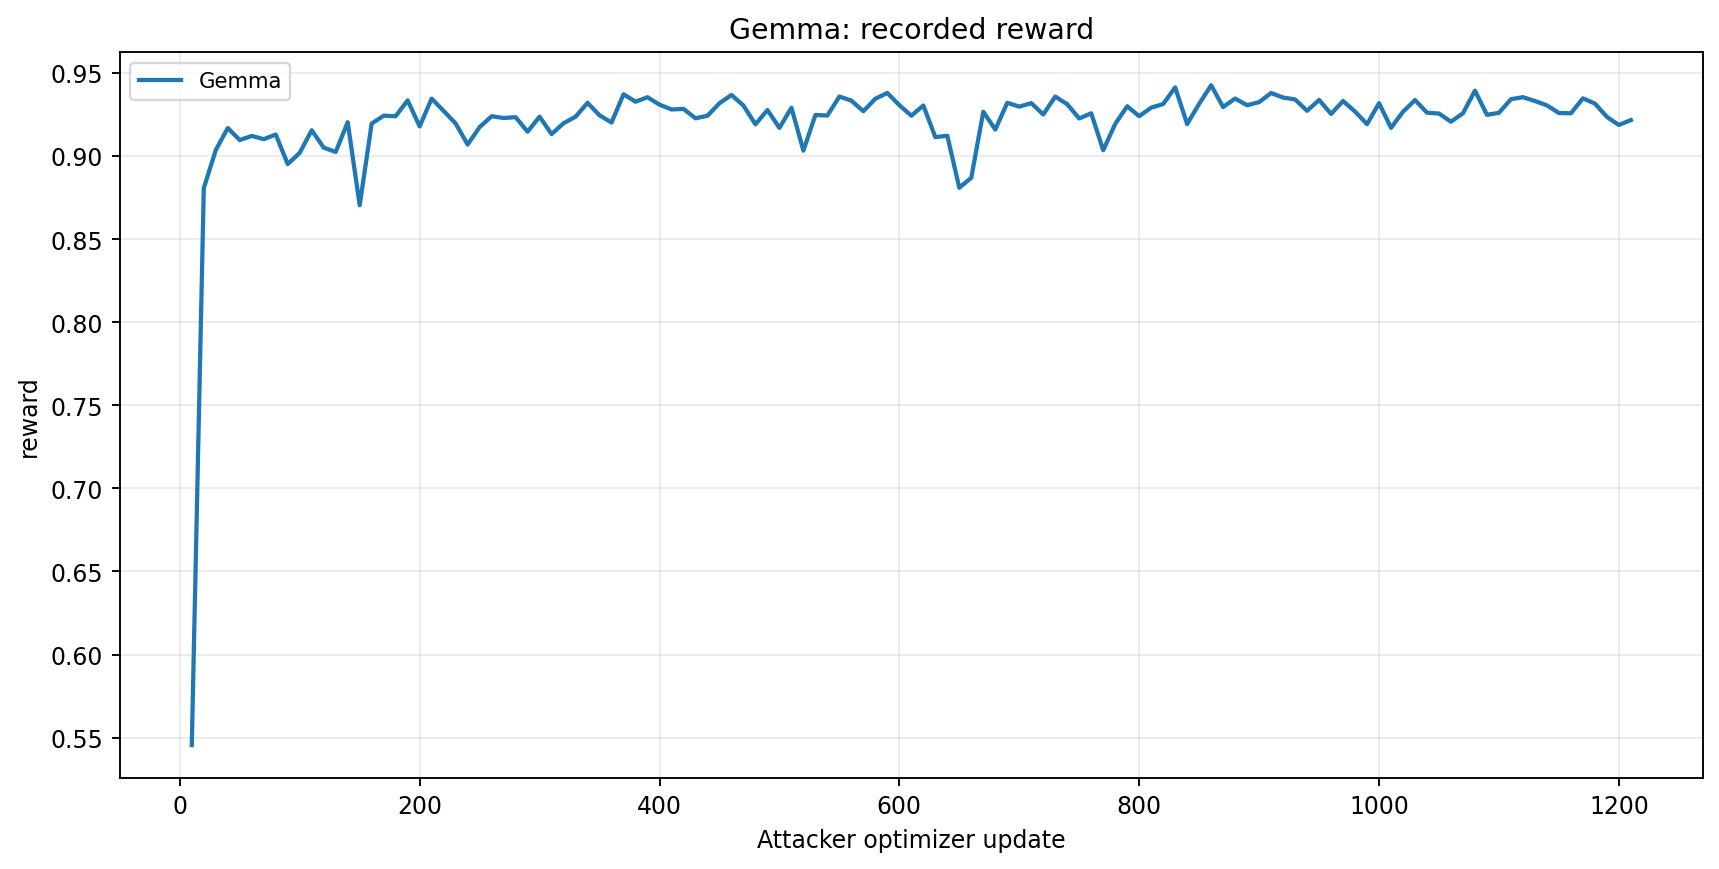
\includegraphics[keepaspectratio,alt={retained-gemma-reward}]{../docs/figures/research/retained-gemma-reward.png}}
\caption{retained-gemma-reward}
\end{recordfigure}

\href{../docs/figures/research/retained-gemma-reward.csv}{Source CSV} ·
\href{../docs/figures/research/retained-gemma-reward.svg}{Vector SVG}.

\begin{recordfigure}
\centering
\pandocbounded{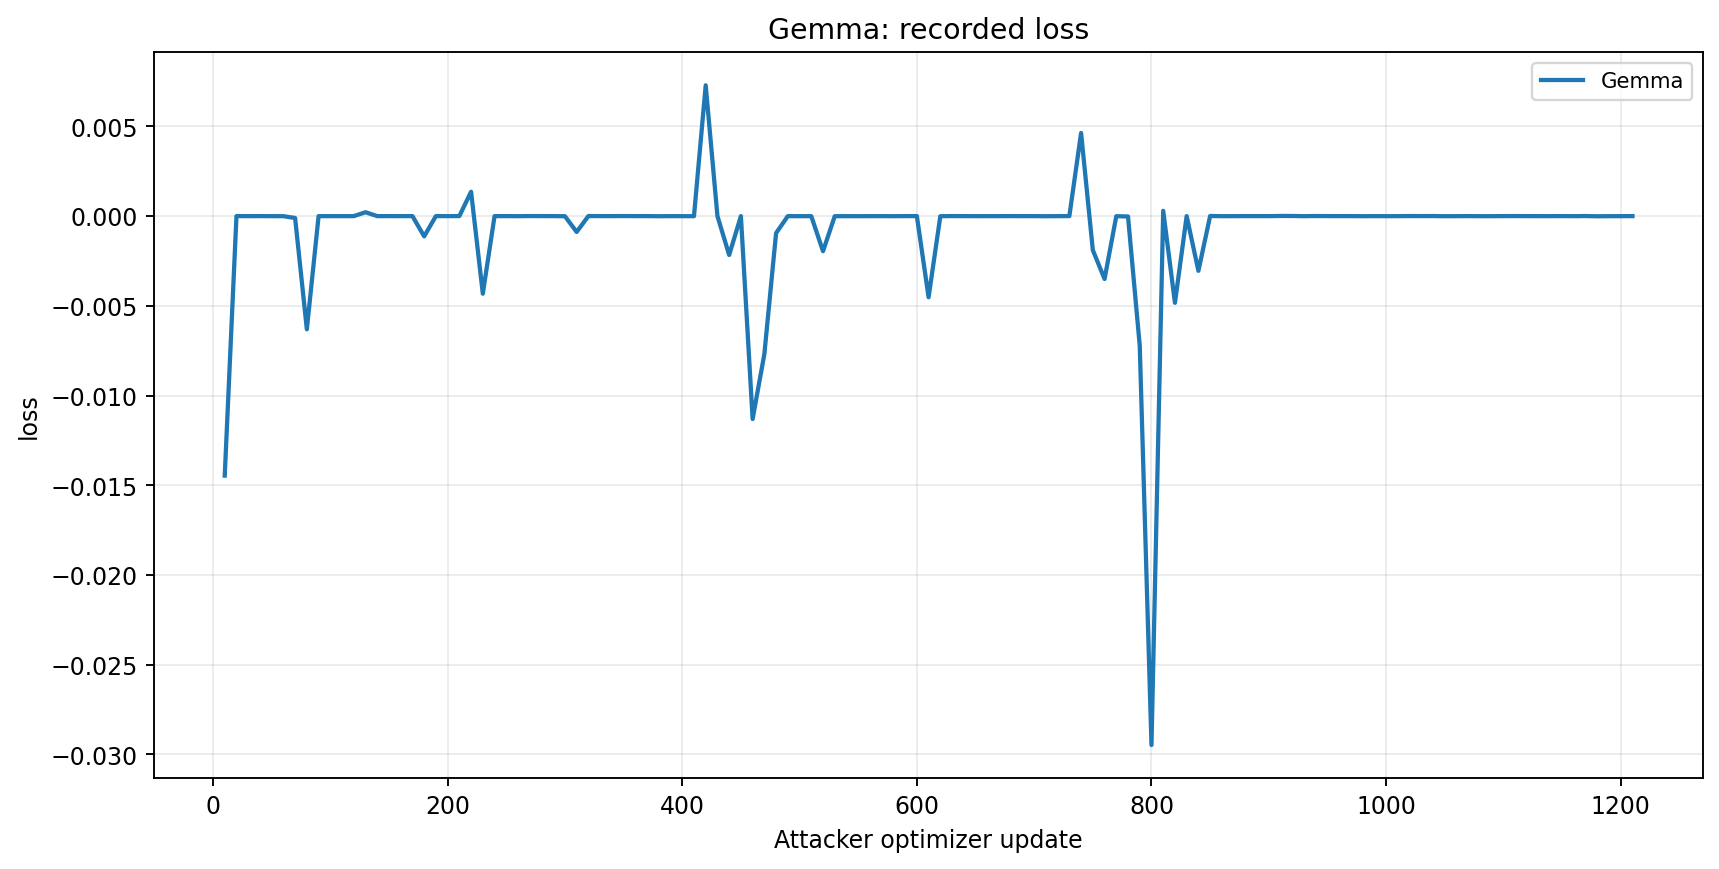
\includegraphics[keepaspectratio,alt={retained-gemma-loss}]{../docs/figures/research/retained-gemma-loss.png}}
\caption{retained-gemma-loss}
\end{recordfigure}

\href{../docs/figures/research/retained-gemma-loss.csv}{Source CSV} ·
\href{../docs/figures/research/retained-gemma-loss.svg}{Vector SVG}.

\begin{recordfigure}
\centering
\pandocbounded{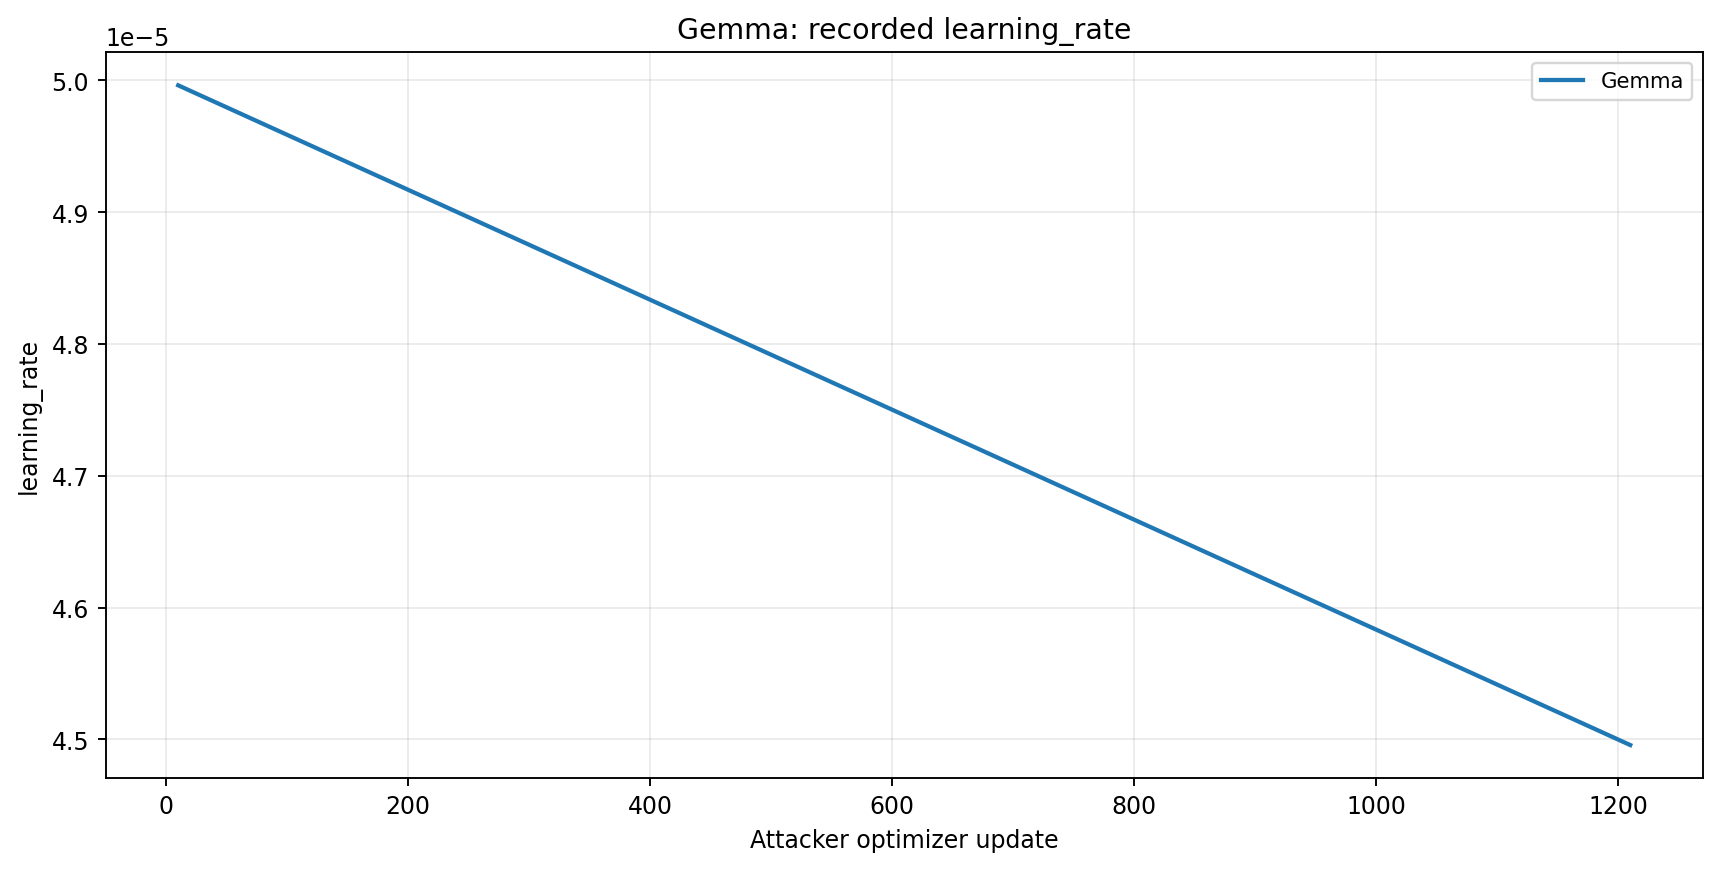
\includegraphics[keepaspectratio,alt={}]{../docs/figures/research/retained-gemma-learning_rate.png}}
\caption{retained-gemma-learning\_\allowbreak{}rate}
\end{recordfigure}

\href{../docs/figures/research/retained-gemma-learning_rate.csv}{Source
CSV} ·
\href{../docs/figures/research/retained-gemma-learning_rate.svg}{Vector
SVG}.

\subsection{ModernBERT-large: retained
checkpoints}\label{record-docs-research-results-md-modernbert-large-retained-checkpoints}

Step 500:
\texttt{\seqsplit{/lustre/fswork/projects/rech/mbm/ual37ci/bench\_research\_ml\_project/split-repos/ai-content-robustness/results/research\_workflow/defender\_comparison/rl/encoder/milestones/step\_500}}.

Final saved attacker:
\texttt{\seqsplit{/lustre/fswork/projects/rech/mbm/ual37ci/bench\_research\_ml\_project/split-repos/ai-content-robustness/results/research\_workflow/defender\_comparison/rl/encoder/checkpoint-1487}}
at 1487 updates.

\begin{recordfigure}
\centering
\pandocbounded{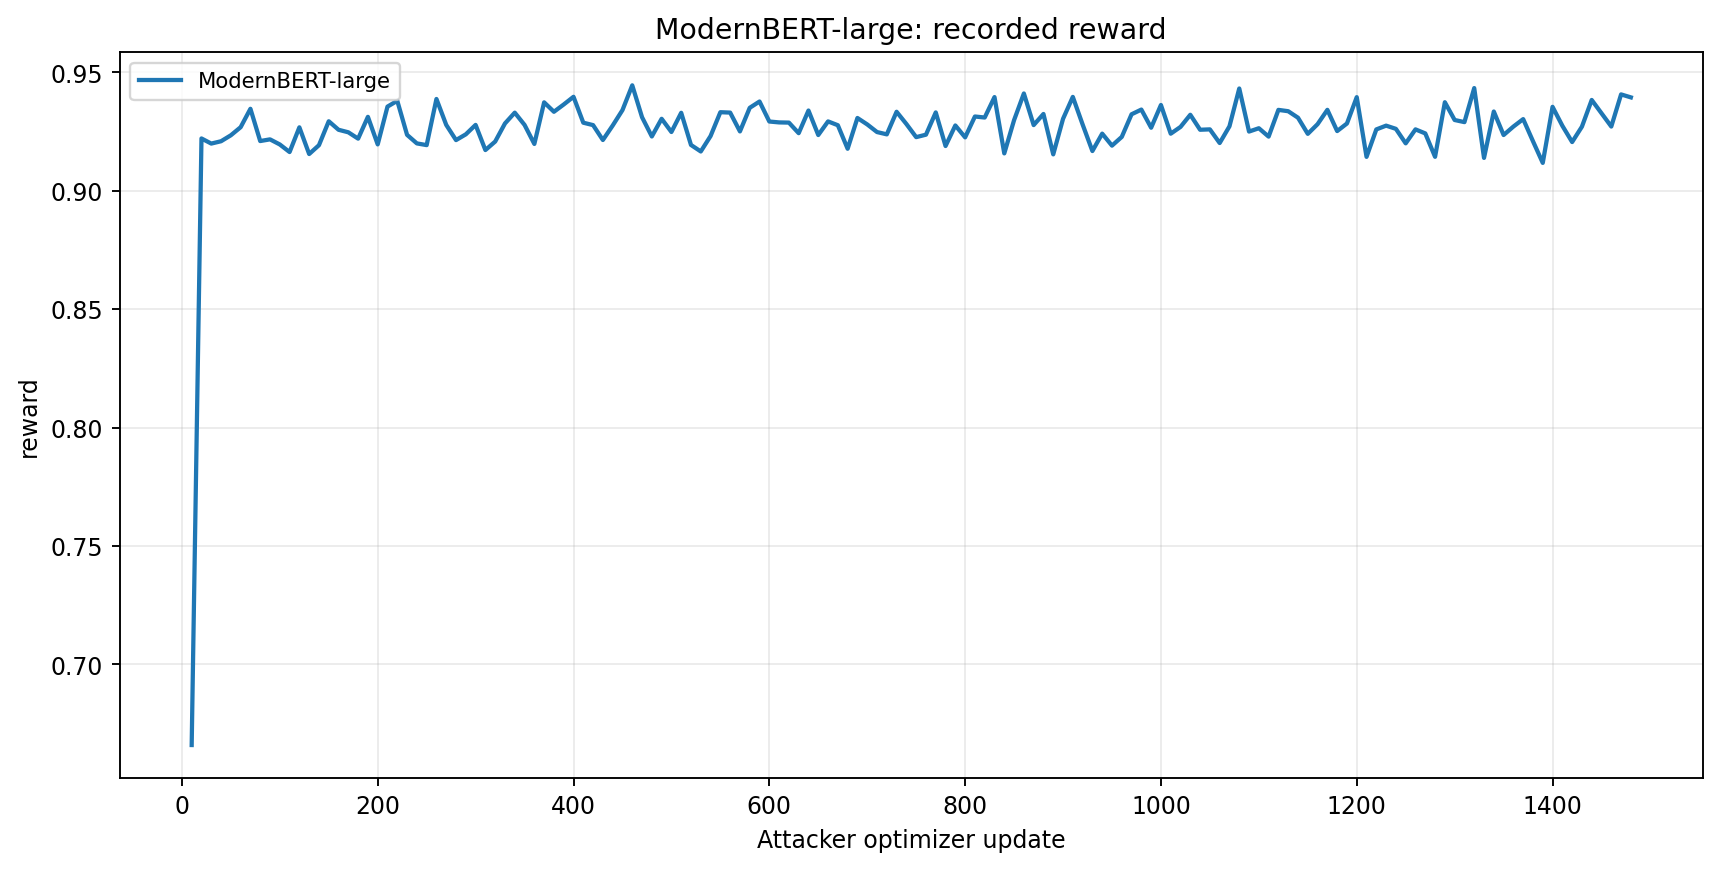
\includegraphics[keepaspectratio,alt={retained-modernbert-reward}]{../docs/figures/research/retained-modernbert-reward.png}}
\caption{retained-modernbert-reward}
\end{recordfigure}

\href{../docs/figures/research/retained-modernbert-reward.csv}{Source
CSV} ·
\href{../docs/figures/research/retained-modernbert-reward.svg}{Vector
SVG}.

\begin{recordfigure}
\centering
\pandocbounded{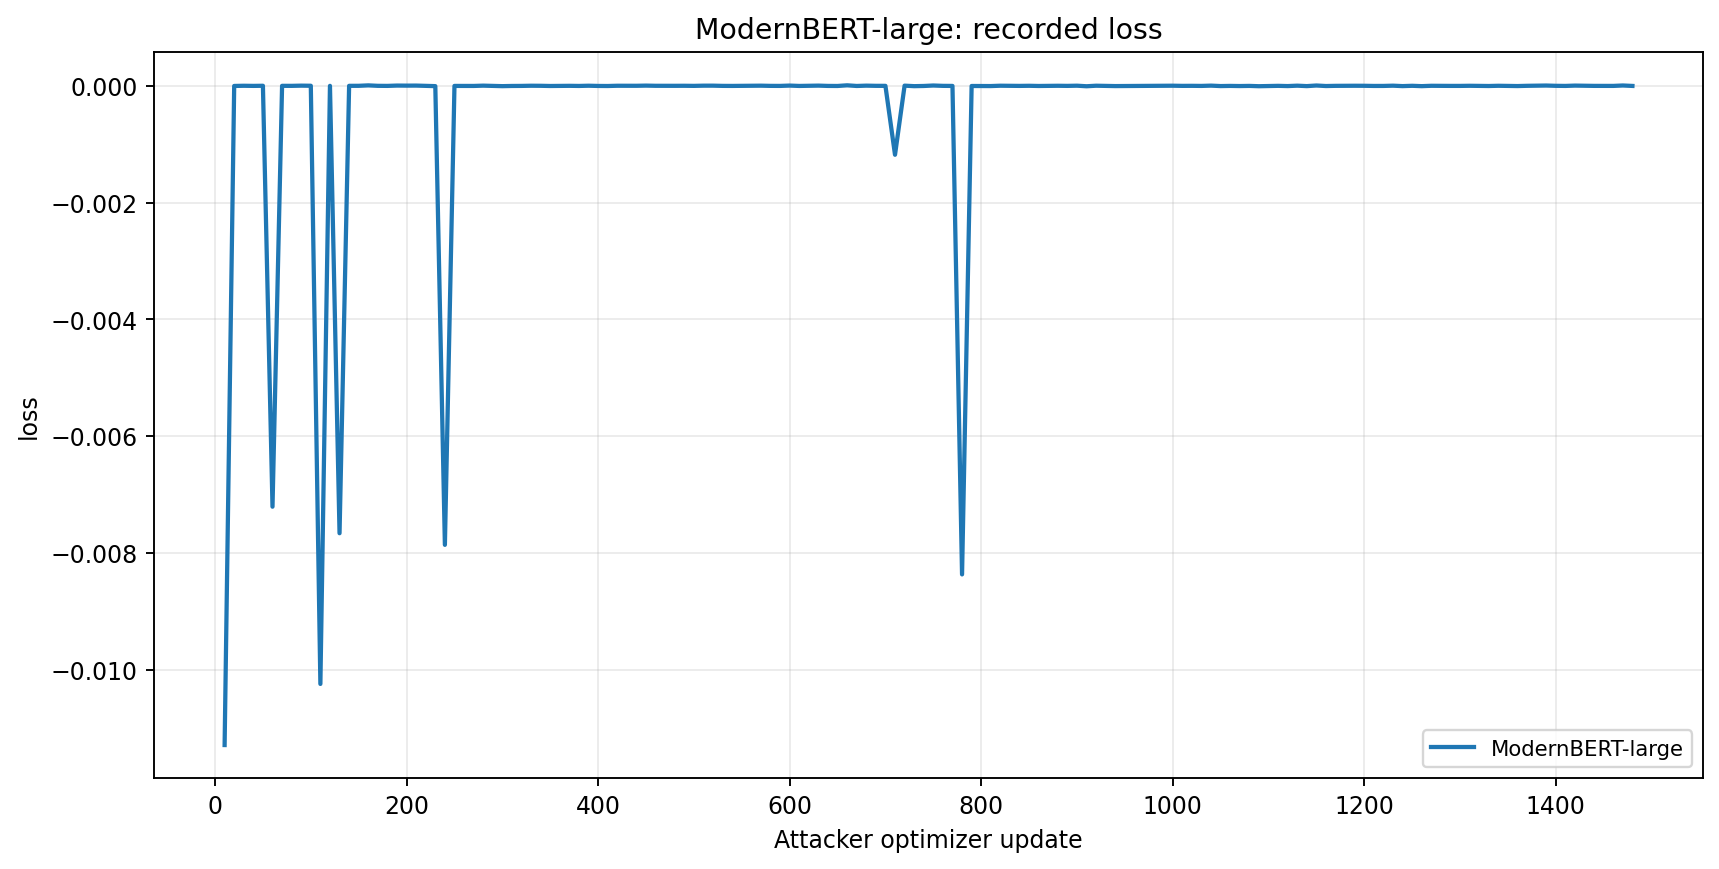
\includegraphics[keepaspectratio,alt={retained-modernbert-loss}]{../docs/figures/research/retained-modernbert-loss.png}}
\caption{retained-modernbert-loss}
\end{recordfigure}

\href{../docs/figures/research/retained-modernbert-loss.csv}{Source CSV}
· \href{../docs/figures/research/retained-modernbert-loss.svg}{Vector
SVG}.

\begin{recordfigure}
\centering
\pandocbounded{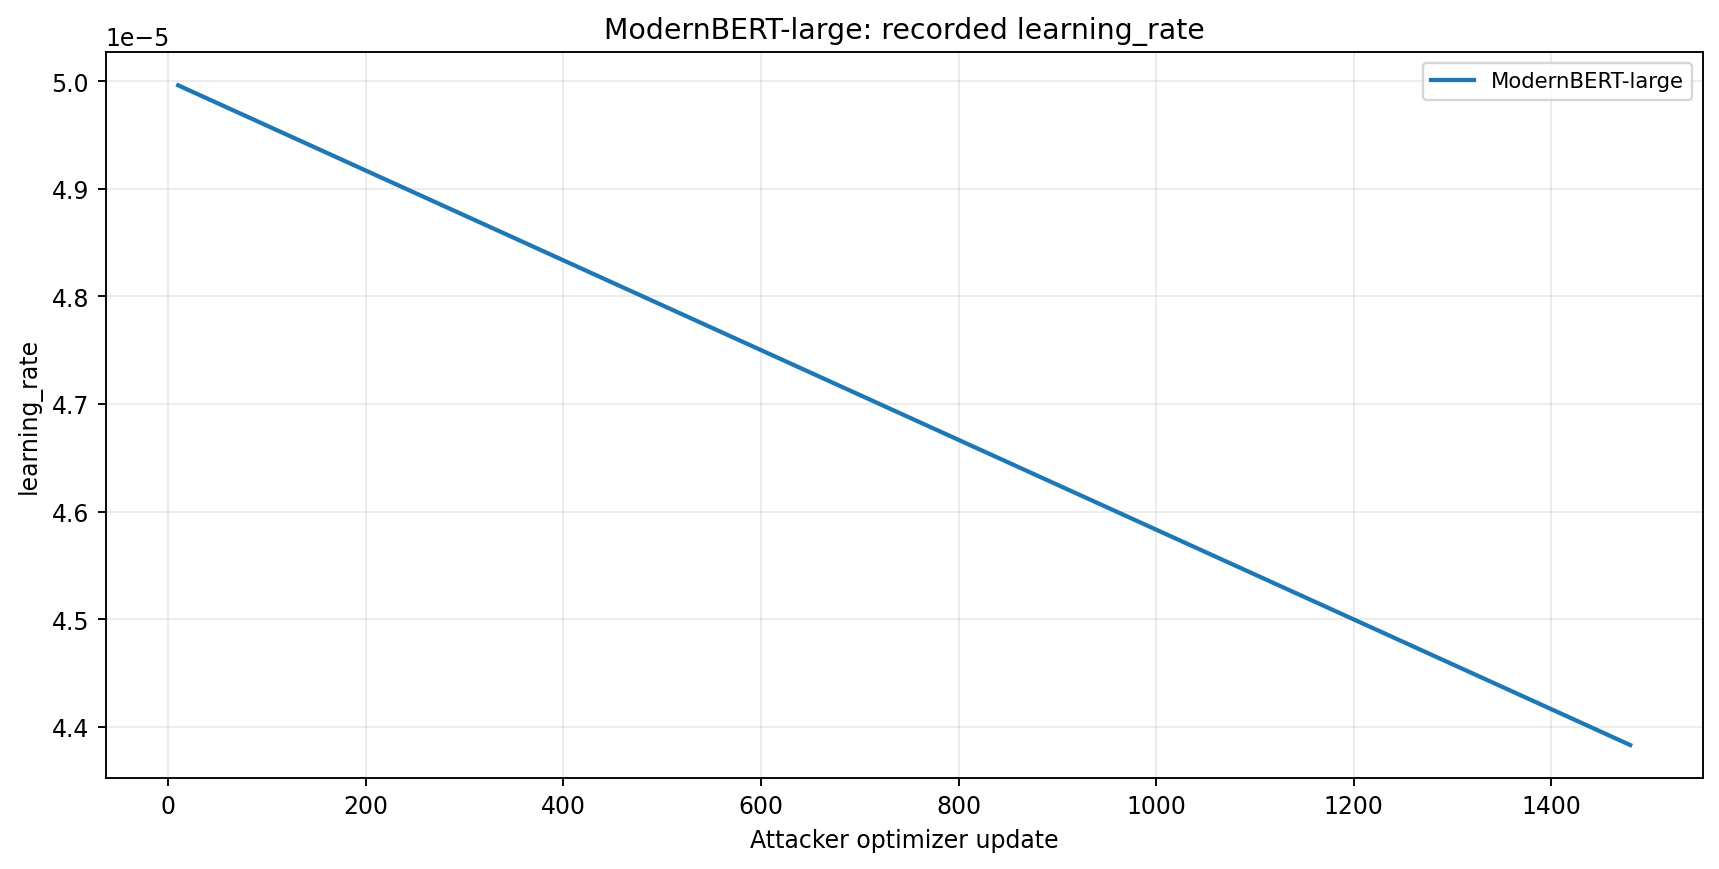
\includegraphics[keepaspectratio,alt={}]{../docs/figures/research/retained-modernbert-learning_rate.png}}
\caption{retained-modernbert-learning\_\allowbreak{}rate}
\end{recordfigure}

\href{../docs/figures/research/retained-modernbert-learning_rate.csv}{Source
CSV} ·
\href{../docs/figures/research/retained-modernbert-learning_rate.svg}{Vector
SVG}.

\subsection{Seven-detector ensemble: retained
checkpoints}\label{record-docs-research-results-md-seven-detector-ensemble-retained-checkpoints}

Step 500:
\texttt{\seqsplit{/lustre/fswork/projects/rech/mbm/ual37ci/bench\_research\_ml\_project/split-repos/ai-content-robustness/results/research\_workflow/defender\_comparison/rl/ensemble/checkpoint-500}}.

Final saved attacker:
\texttt{\seqsplit{/lustre/fswork/projects/rech/mbm/ual37ci/bench\_research\_ml\_project/split-repos/ai-content-robustness/results/research\_workflow/defender\_comparison/rl/ensemble/checkpoint-502}}
at 502 updates.

\begin{recordfigure}
\centering
\pandocbounded{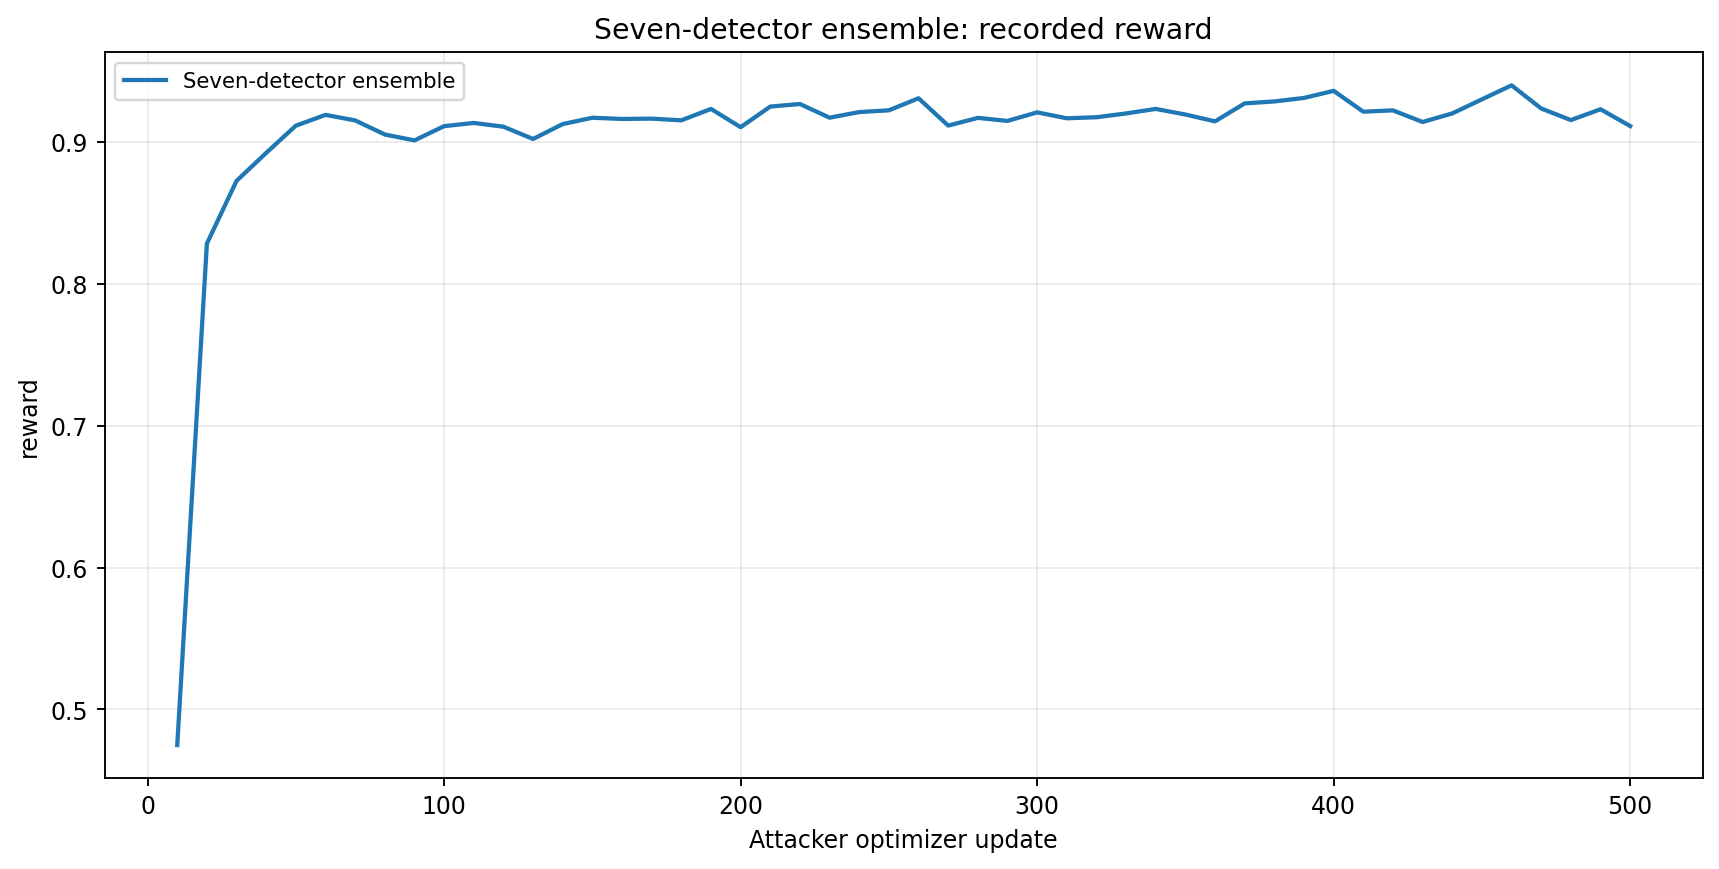
\includegraphics[keepaspectratio,alt={retained-ensemble-reward}]{../docs/figures/research/retained-ensemble-reward.png}}
\caption{retained-ensemble-reward}
\end{recordfigure}

\href{../docs/figures/research/retained-ensemble-reward.csv}{Source CSV}
· \href{../docs/figures/research/retained-ensemble-reward.svg}{Vector
SVG}.

\begin{recordfigure}
\centering
\pandocbounded{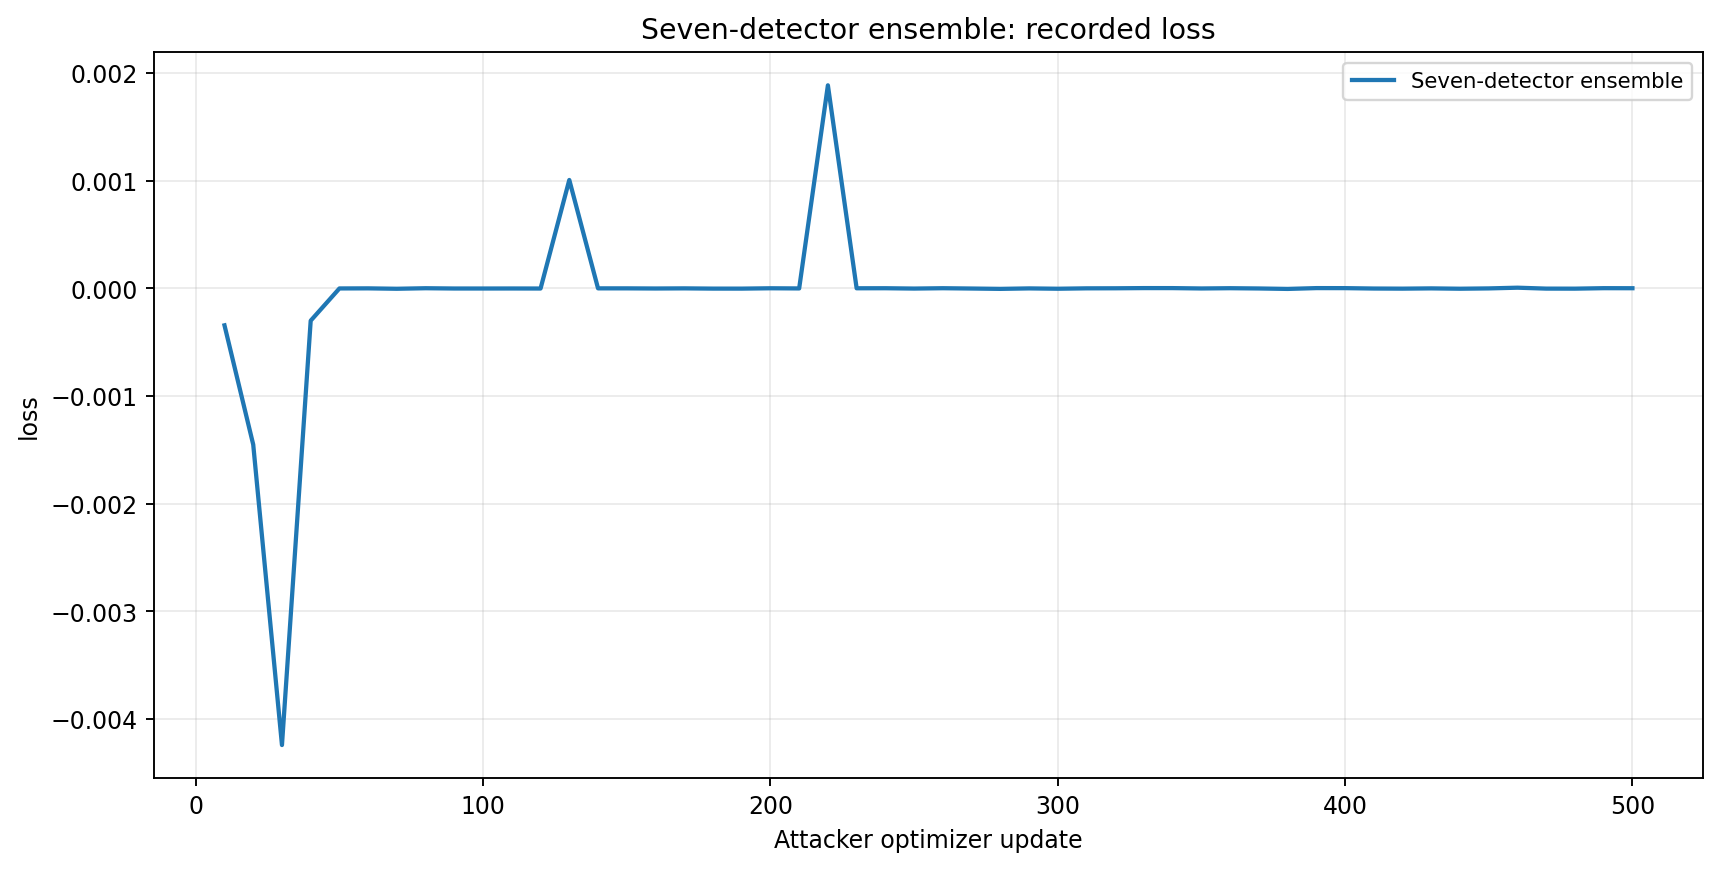
\includegraphics[keepaspectratio,alt={retained-ensemble-loss}]{../docs/figures/research/retained-ensemble-loss.png}}
\caption{retained-ensemble-loss}
\end{recordfigure}

\href{../docs/figures/research/retained-ensemble-loss.csv}{Source CSV} ·
\href{../docs/figures/research/retained-ensemble-loss.svg}{Vector SVG}.

\begin{recordfigure}
\centering
\pandocbounded{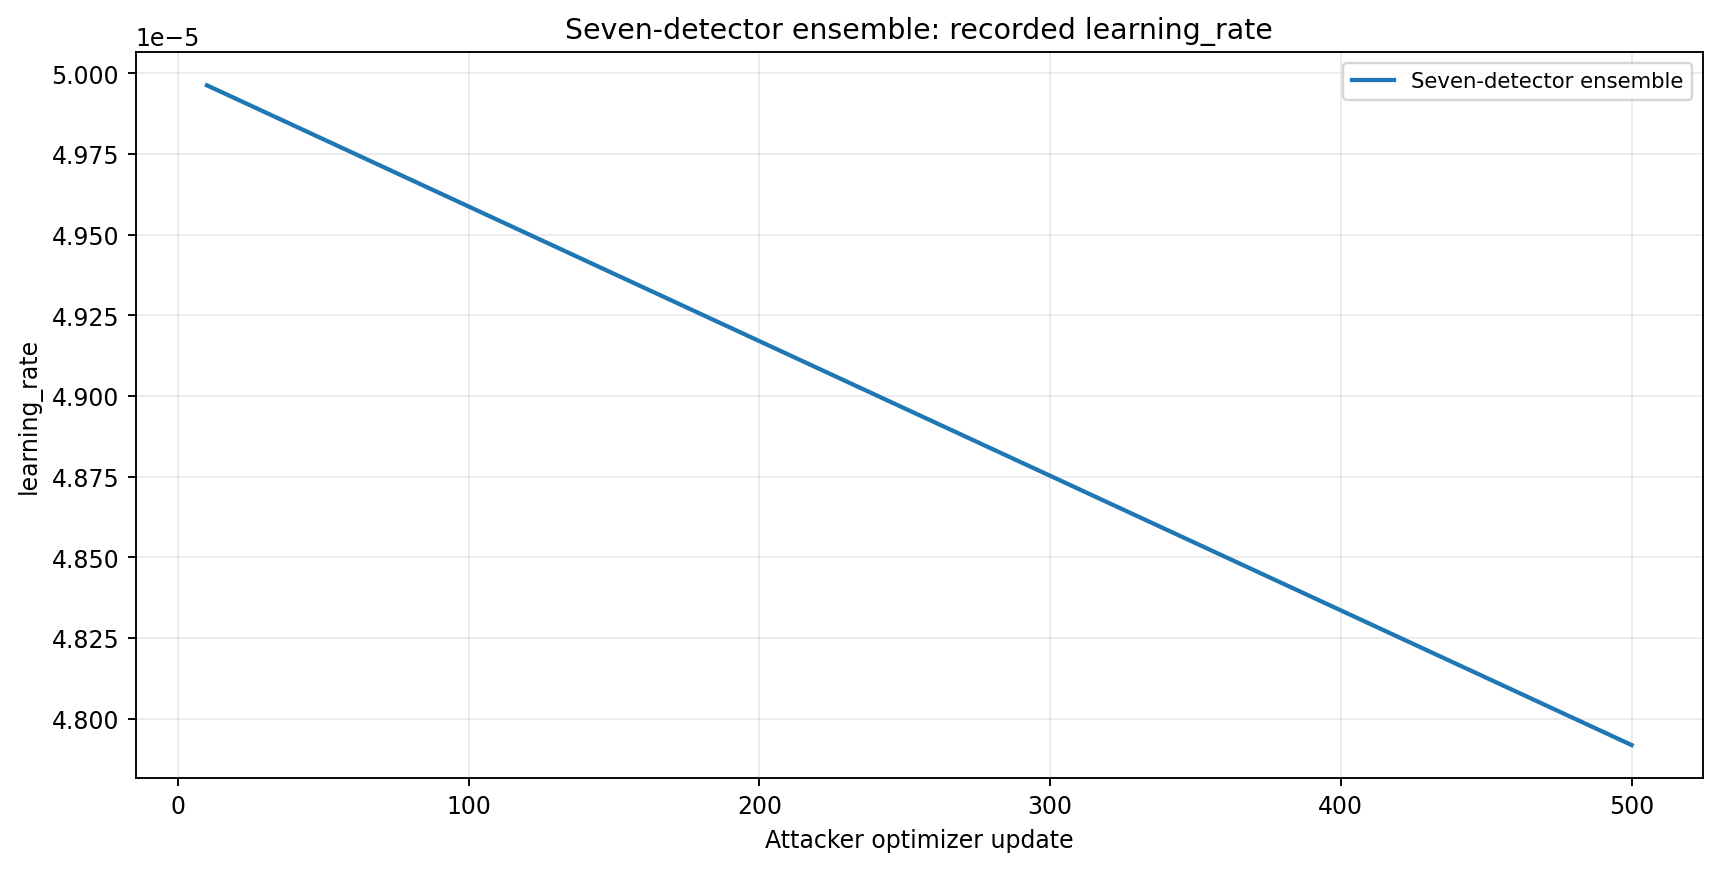
\includegraphics[keepaspectratio,alt={}]{../docs/figures/research/retained-ensemble-learning_rate.png}}
\caption{retained-ensemble-learning\_\allowbreak{}rate}
\end{recordfigure}

\href{../docs/figures/research/retained-ensemble-learning_rate.csv}{Source
CSV} ·
\href{../docs/figures/research/retained-ensemble-learning_rate.svg}{Vector
SVG}.

\subsection{RoBERTa: retained
checkpoints}\label{record-docs-research-results-md-roberta-retained-checkpoints}

Step 500:
\texttt{\seqsplit{/lustre/fswork/projects/rech/mbm/ual37ci/bench\_research\_ml\_project/split-repos/ai-content-robustness/results/research\_workflow/defender\_comparison/retained\_attackers/roberta/checkpoint-500}}.

\begin{recordfigure}
\centering
\pandocbounded{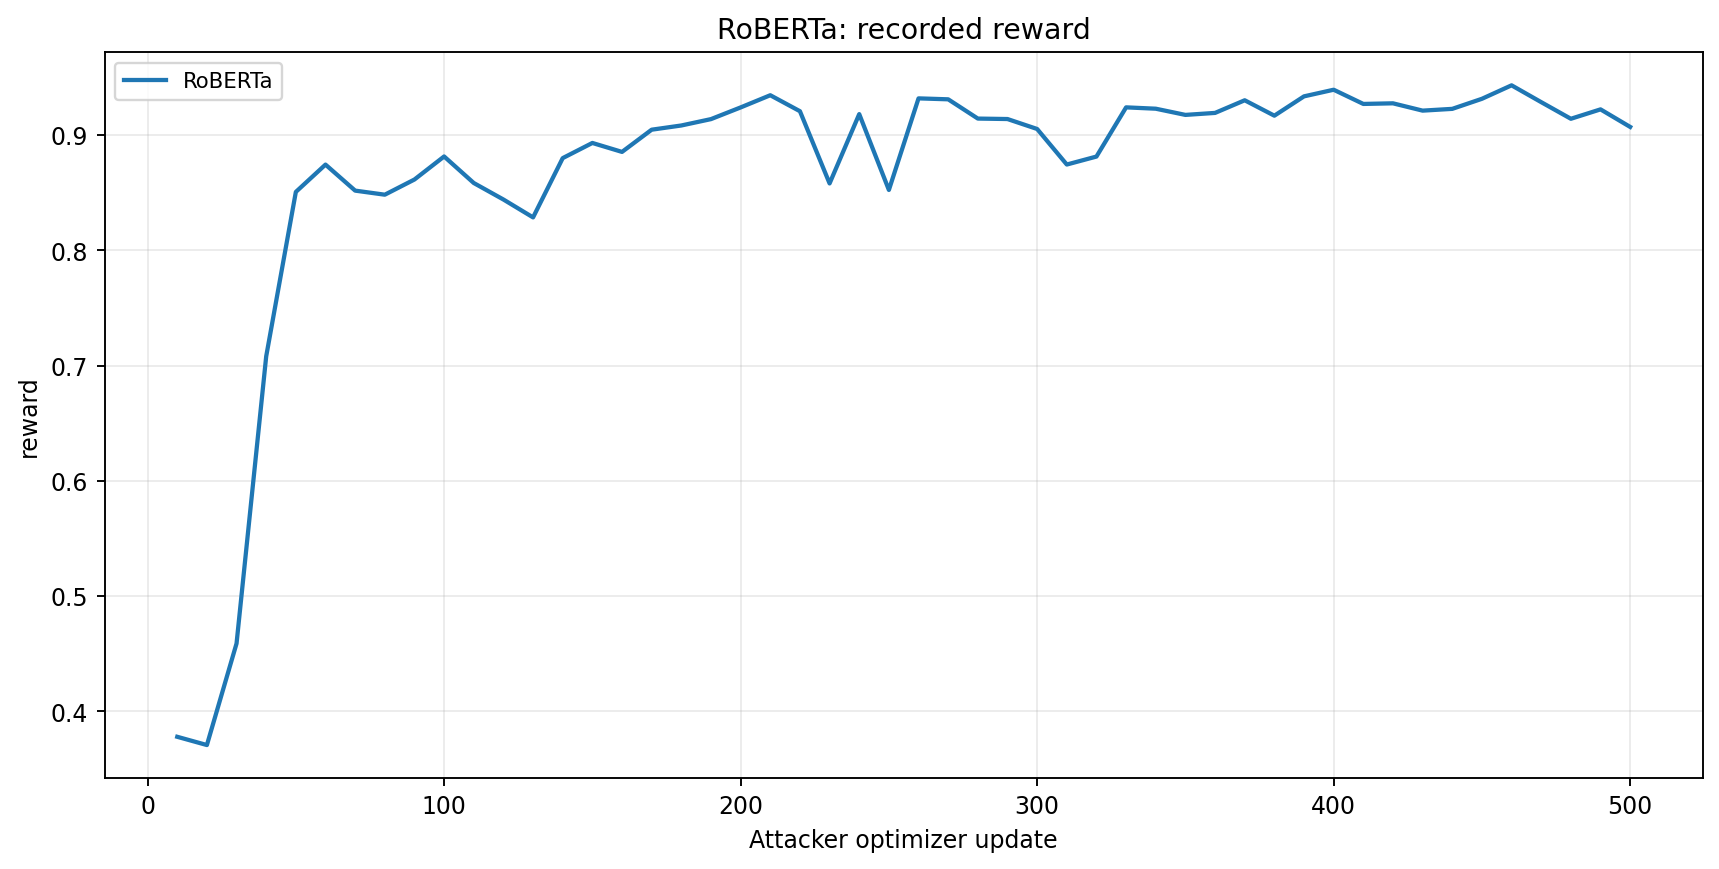
\includegraphics[keepaspectratio,alt={retained-roberta-reward}]{../docs/figures/research/retained-roberta-reward.png}}
\caption{retained-roberta-reward}
\end{recordfigure}

\href{../docs/figures/research/retained-roberta-reward.csv}{Source CSV}
· \href{../docs/figures/research/retained-roberta-reward.svg}{Vector
SVG}.

\begin{recordfigure}
\centering
\pandocbounded{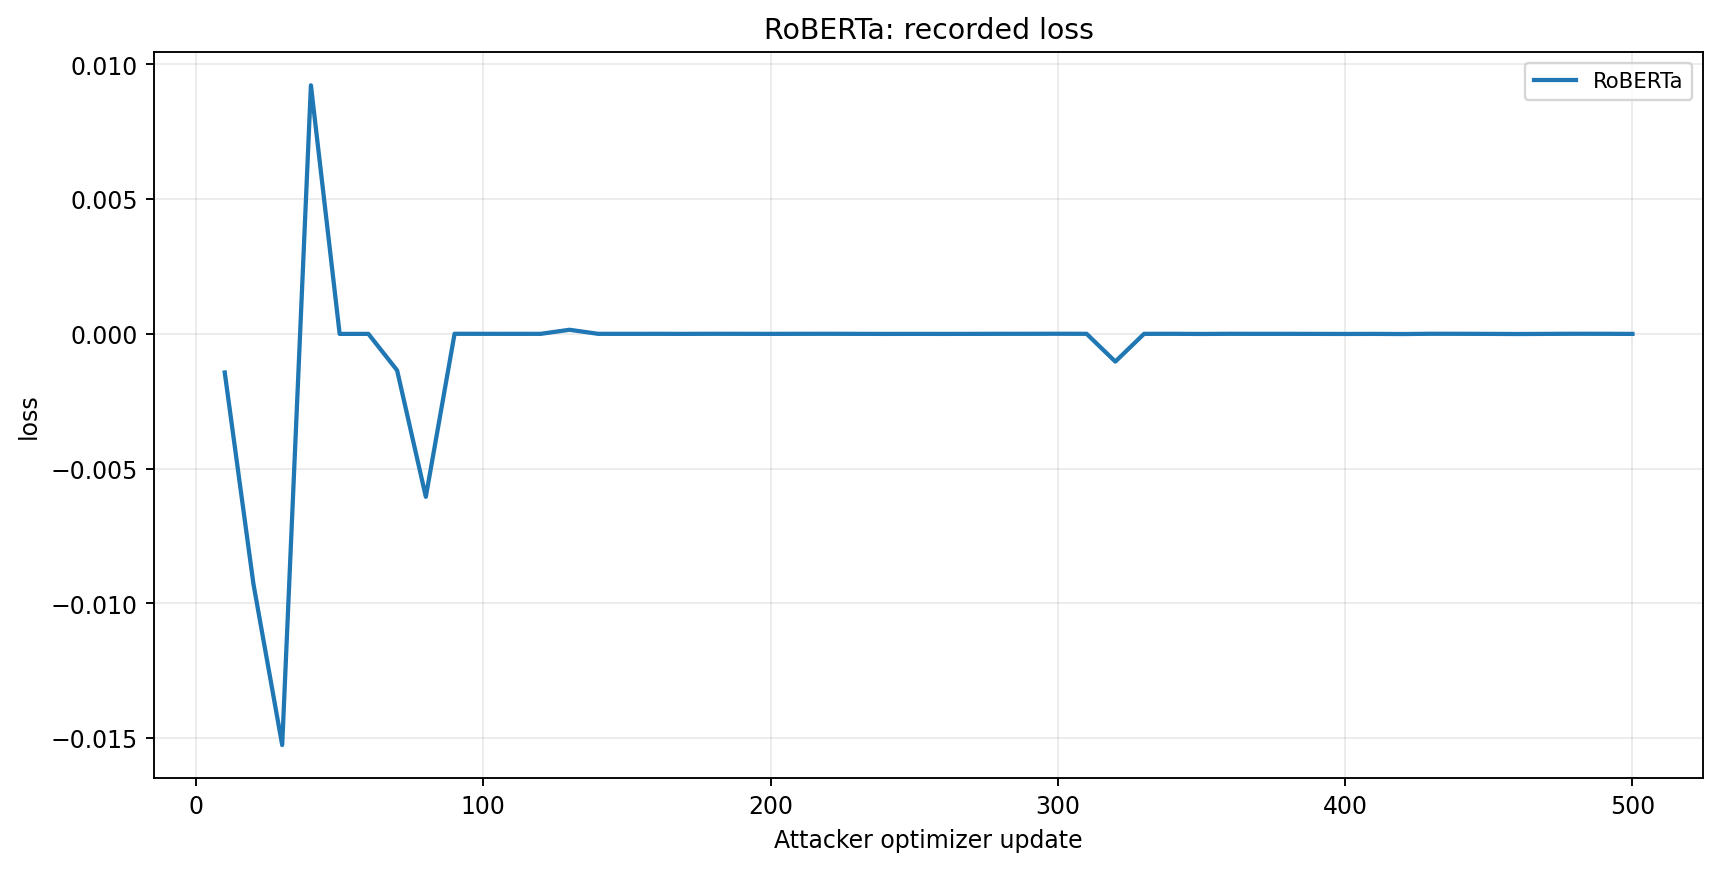
\includegraphics[keepaspectratio,alt={retained-roberta-loss}]{../docs/figures/research/retained-roberta-loss.png}}
\caption{retained-roberta-loss}
\end{recordfigure}

\href{../docs/figures/research/retained-roberta-loss.csv}{Source CSV} ·
\href{../docs/figures/research/retained-roberta-loss.svg}{Vector SVG}.

\begin{recordfigure}
\centering
\pandocbounded{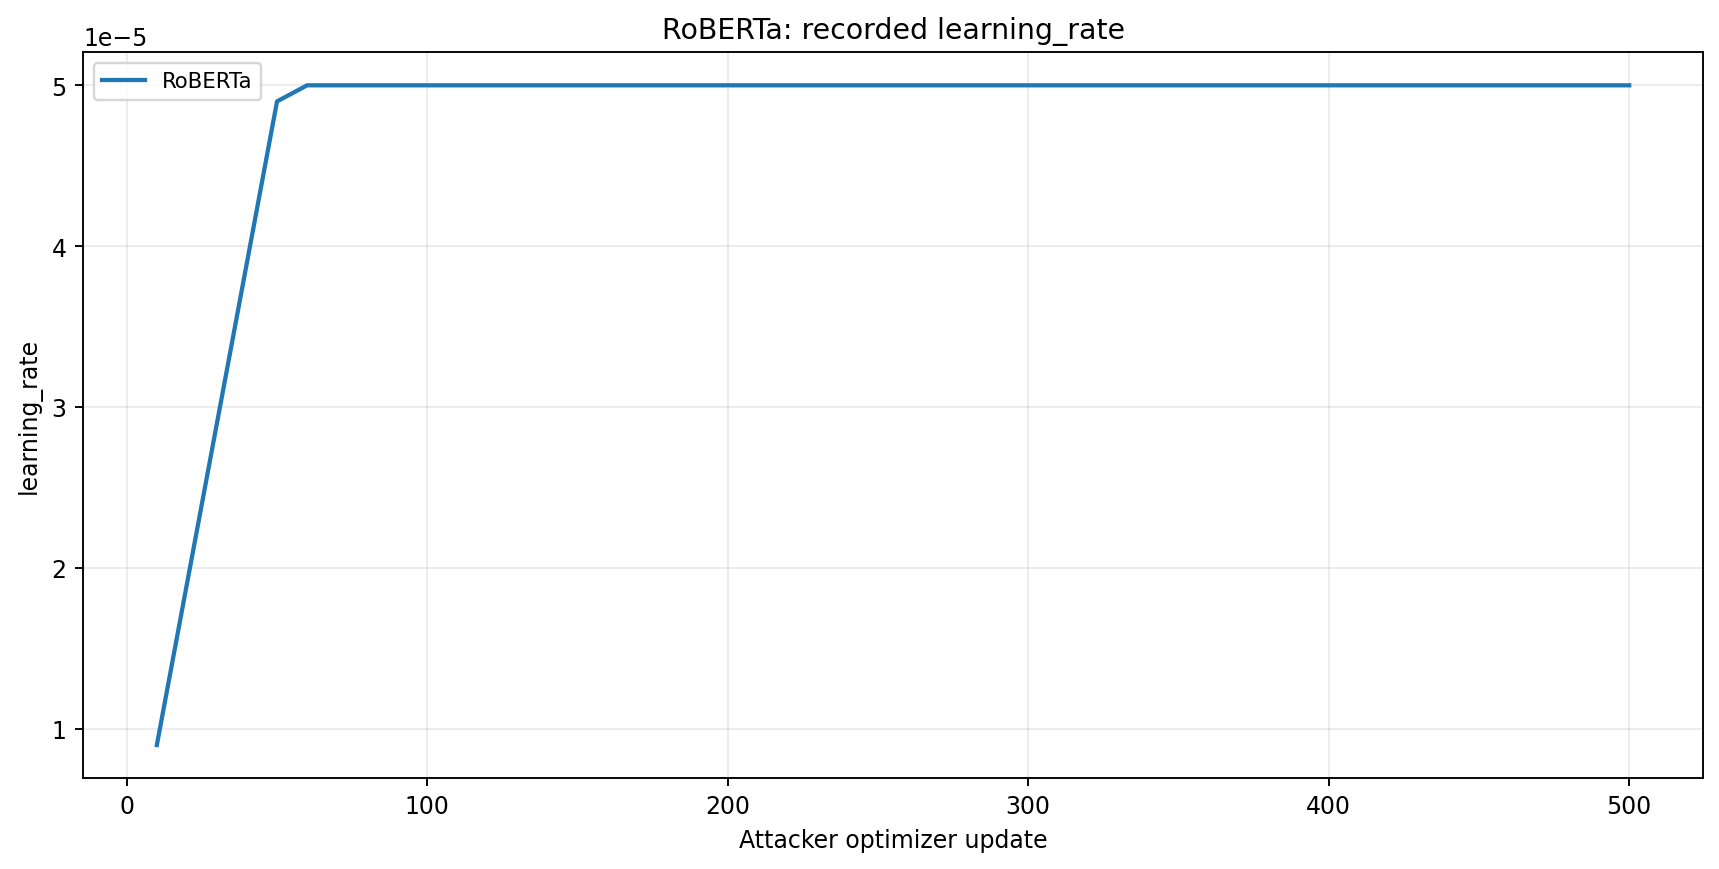
\includegraphics[keepaspectratio,alt={}]{../docs/figures/research/retained-roberta-learning_rate.png}}
\caption{retained-roberta-learning\_\allowbreak{}rate}
\end{recordfigure}

\href{../docs/figures/research/retained-roberta-learning_rate.csv}{Source
CSV} ·
\href{../docs/figures/research/retained-roberta-learning_rate.svg}{Vector
SVG}.

{\scriptsize\setlength{\tabcolsep}{3pt}\def\LTcaptype{none} % do not increment counter
\begin{longtable}[]{@{}
  >{\raggedright\arraybackslash}p{(\linewidth - 4\tabcolsep) * \real{0.3333}}
  >{\raggedright\arraybackslash}p{(\linewidth - 4\tabcolsep) * \real{0.3333}}
  >{\raggedright\arraybackslash}p{(\linewidth - 4\tabcolsep) * \real{0.3333}}@{}}
\toprule\noalign{}
\begin{minipage}[b]{\linewidth}\raggedright
updates
\end{minipage} & \begin{minipage}[b]{\linewidth}\raggedright
generated\_\allowbreak{}texts
\end{minipage} & \begin{minipage}[b]{\linewidth}\raggedright
evasion
\end{minipage} \\
\midrule\noalign{}
\endhead
\bottomrule\noalign{}
\endlastfoot
0 & 100 & 0.0000 \\
50 & 100 & 0.0000 \\
100 & 100 & 0.0000 \\
150 & 100 & 0.0600 \\
200 & 100 & 0.1900 \\
250 & 100 & 0.1900 \\
300 & 100 & 0.0900 \\
350 & 100 & 0.5900 \\
400 & 100 & 0.8800 \\
450 & 100 & 0.8700 \\
500 & 100 & 0.9800 \\
550 & 100 & 0.9300 \\
600 & 100 & 0.3600 \\
\end{longtable}
}

\begin{recordfigure}
\centering
\pandocbounded{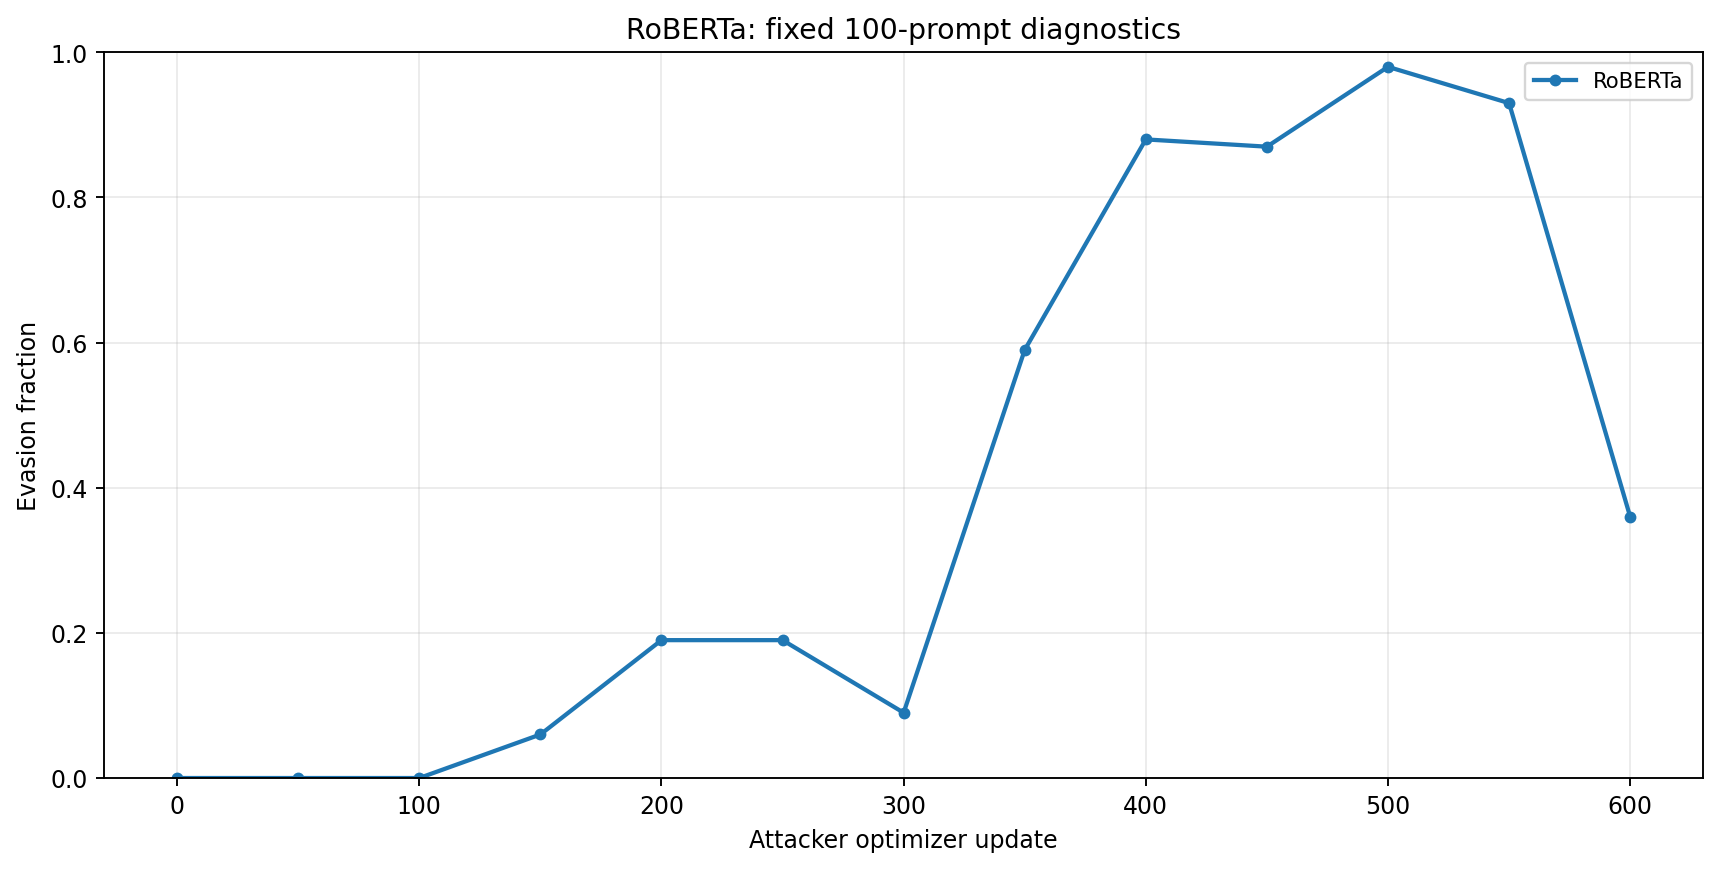
\includegraphics[keepaspectratio,alt={retained-roberta-diagnostic-evasion}]{../docs/figures/research/retained-roberta-diagnostic-evasion.png}}
\caption{retained-roberta-diagnostic-evasion}
\end{recordfigure}

\href{../docs/figures/research/retained-roberta-diagnostic-evasion.csv}{Source
CSV} ·
\href{../docs/figures/research/retained-roberta-diagnostic-evasion.svg}{Vector
SVG}.

The RoBERTa trajectory uses a separate individual-attacker protocol:
50-update warm-up to \texttt{\seqsplit{5e-5}}, then a constant rate
through 600. Evasion was 98\% at 500, 93\% at 550 and 36\% at 600 on the
same 100 prompts. The full 500-text evaluation at 600 gave 39.2\%
evasion. Only the step-500 model is retained; later measurements remain
as evidence of fluctuation. A high score at one checkpoint therefore
does not establish stable convergence.

\subsection{Interpretation
limits}\label{record-docs-research-results-md-interpretation-limits}

Training budgets and target detectors differ across the long runs, so
their final scores are not a matched-budget architecture ranking. These
are single-seed results. The diagnostic evaluation set has informed
protocol choices and is not an untouched final test. The retained
evaluations show evasion against frozen warmed defenders; the new jobs
measure whether defender updates recover detection.

\subsection{Current experiment: one defender update per retained
attacker}\label{record-docs-research-results-md-current-experiment-one-defender-update-per-retained-attacker}

Three independent jobs generate training outputs on the existing 1,000
fitting prompts, pair them with human passages, and update the warmed
defender(s). Torch defenders use the existing three-epoch supervised
update and paired 80/20 training/validation split. The 500 evaluation
prompts are excluded from training. The post-defense measurement reuses
exactly the saved attack texts from the original evaluation. No attacker
optimizer runs and no second round starts in these submissions.

\subsection{Architecture races:
20261022T135029612516Z}\label{record-docs-research-results-md-architecture-races-20261022t135029612516z}

1 planned rounds. One defender update per branch; zero new attacker
updates. Each branch starts from its retained attacker and the original
warmed defender(s). Allocation: 02:00:00; QoS:
qos\_\allowbreak{}gpu\_\allowbreak{}h100-dev. Checkpoint pauses requeue
the same job.

\href{../results/research_workflow/defender_comparison/races_100/20261022T135029612516Z/metrics.csv}{Shared
metrics after every evaluation}. Rows identify the race, round, phase,
detector and cumulative attacker updates. Concurrent writes are locked;
replayed measurements do not add duplicate rows.

\subsubsection{gemma: job
1447844}\label{record-docs-research-results-md-gemma-job-1447844}

Status: completed; completed rounds: 1/1.

Retained attacker:
\texttt{\seqsplit{/lustre/fswork/projects/rech/mbm/ual37ci/bench\_research\_ml\_project/split-repos/ai-content-robustness/results/research\_workflow/defender\_comparison/rl/decoder/checkpoint-1213}},
trained for \textbf{1213 updates}. Initial evaluations reuse the saved
texts and scores after identity checks. Post-defense evaluation reuses
exactly those attack texts.

{\scriptsize\setlength{\tabcolsep}{3pt}\def\LTcaptype{none} % do not increment counter
\begin{longtable}[]{@{}
  >{\raggedright\arraybackslash}p{(\linewidth - 8\tabcolsep) * \real{0.2000}}
  >{\raggedright\arraybackslash}p{(\linewidth - 8\tabcolsep) * \real{0.2000}}
  >{\raggedright\arraybackslash}p{(\linewidth - 8\tabcolsep) * \real{0.2000}}
  >{\raggedright\arraybackslash}p{(\linewidth - 8\tabcolsep) * \real{0.2000}}
  >{\raggedright\arraybackslash}p{(\linewidth - 8\tabcolsep) * \real{0.2000}}@{}}
\toprule\noalign{}
\begin{minipage}[b]{\linewidth}\raggedright
round
\end{minipage} & \begin{minipage}[b]{\linewidth}\raggedright
detector
\end{minipage} & \begin{minipage}[b]{\linewidth}\raggedright
before
\end{minipage} & \begin{minipage}[b]{\linewidth}\raggedright
after\_\allowbreak{}attack
\end{minipage} & \begin{minipage}[b]{\linewidth}\raggedright
after\_\allowbreak{}defense
\end{minipage} \\
\midrule\noalign{}
\endhead
\bottomrule\noalign{}
\endlastfoot
1 & decoder\_\allowbreak{}classifier & 0.0000 & 0.7720 & 0.0020 \\
1 & ensemble\_\allowbreak{}mean & 0.0000 & 0.7720 & 0.0020 \\
\end{longtable}
}

\begin{recordfigure}
\centering
\pandocbounded{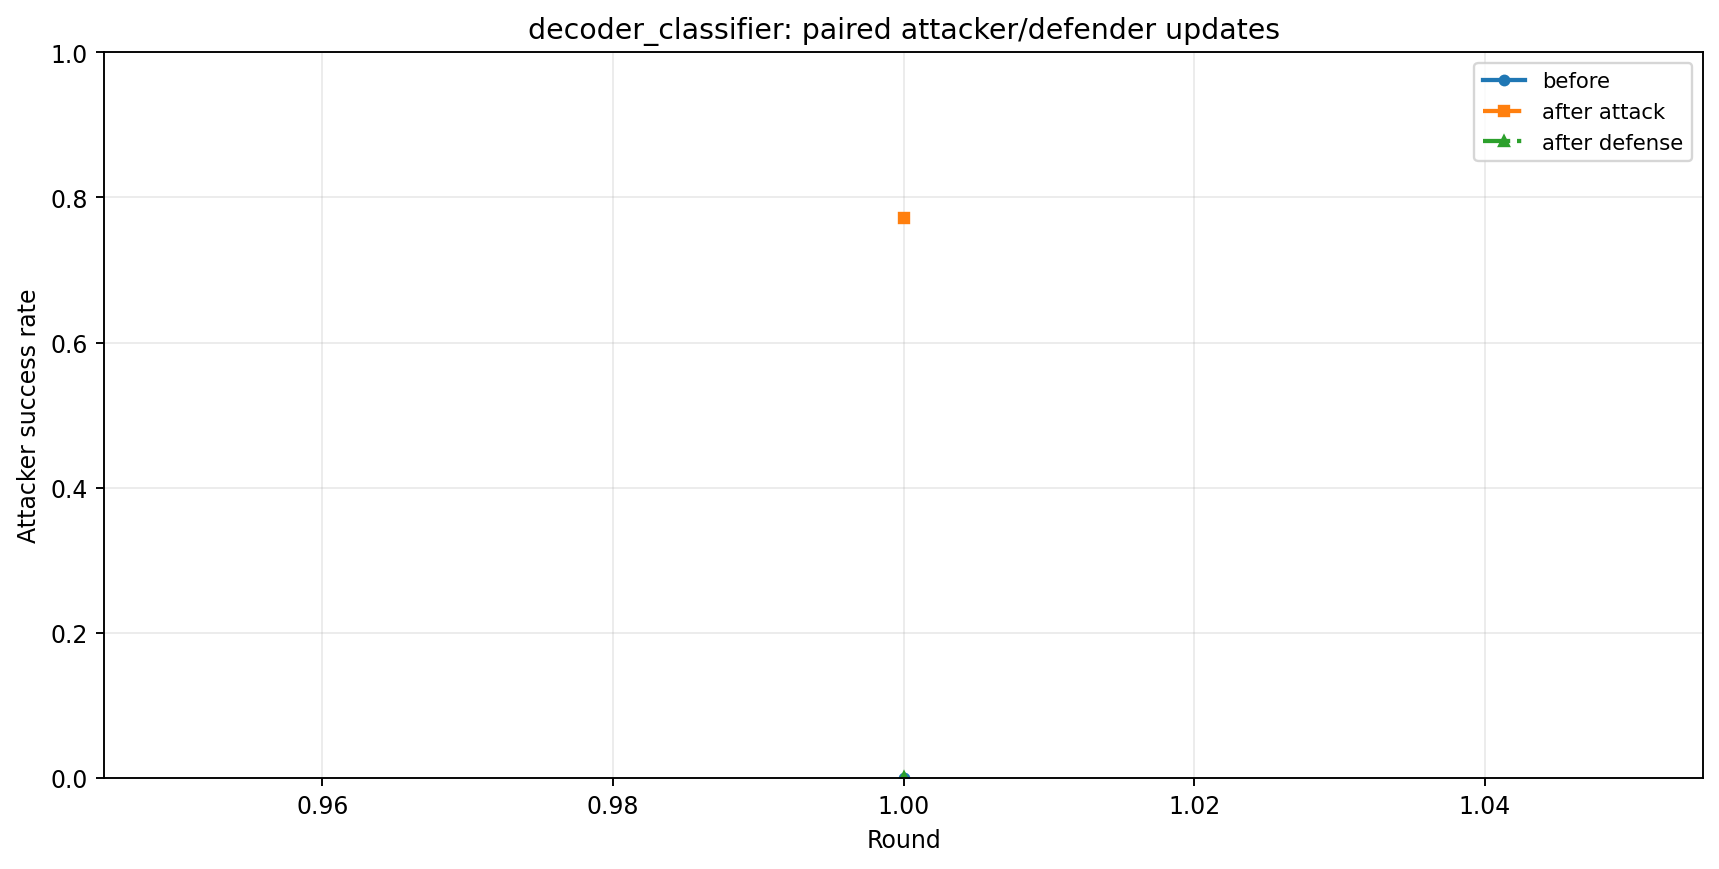
\includegraphics[keepaspectratio,alt={The after-attack and after-defense measurements reuse identical generated texts.}]{../docs/figures/research/race100-20261022T135029612516Z-gemma-decoder_classifier.png}}
\caption{The after-attack and after-defense measurements reuse identical
generated texts.}
\end{recordfigure}

The after-attack and after-defense measurements reuse identical
generated texts.
\href{../docs/figures/research/race100-20261022T135029612516Z-gemma-decoder_classifier.csv}{Source
CSV} ·
\href{../docs/figures/research/race100-20261022T135029612516Z-gemma-decoder_classifier.svg}{Vector
SVG}

\begin{recordfigure}
\centering
\pandocbounded{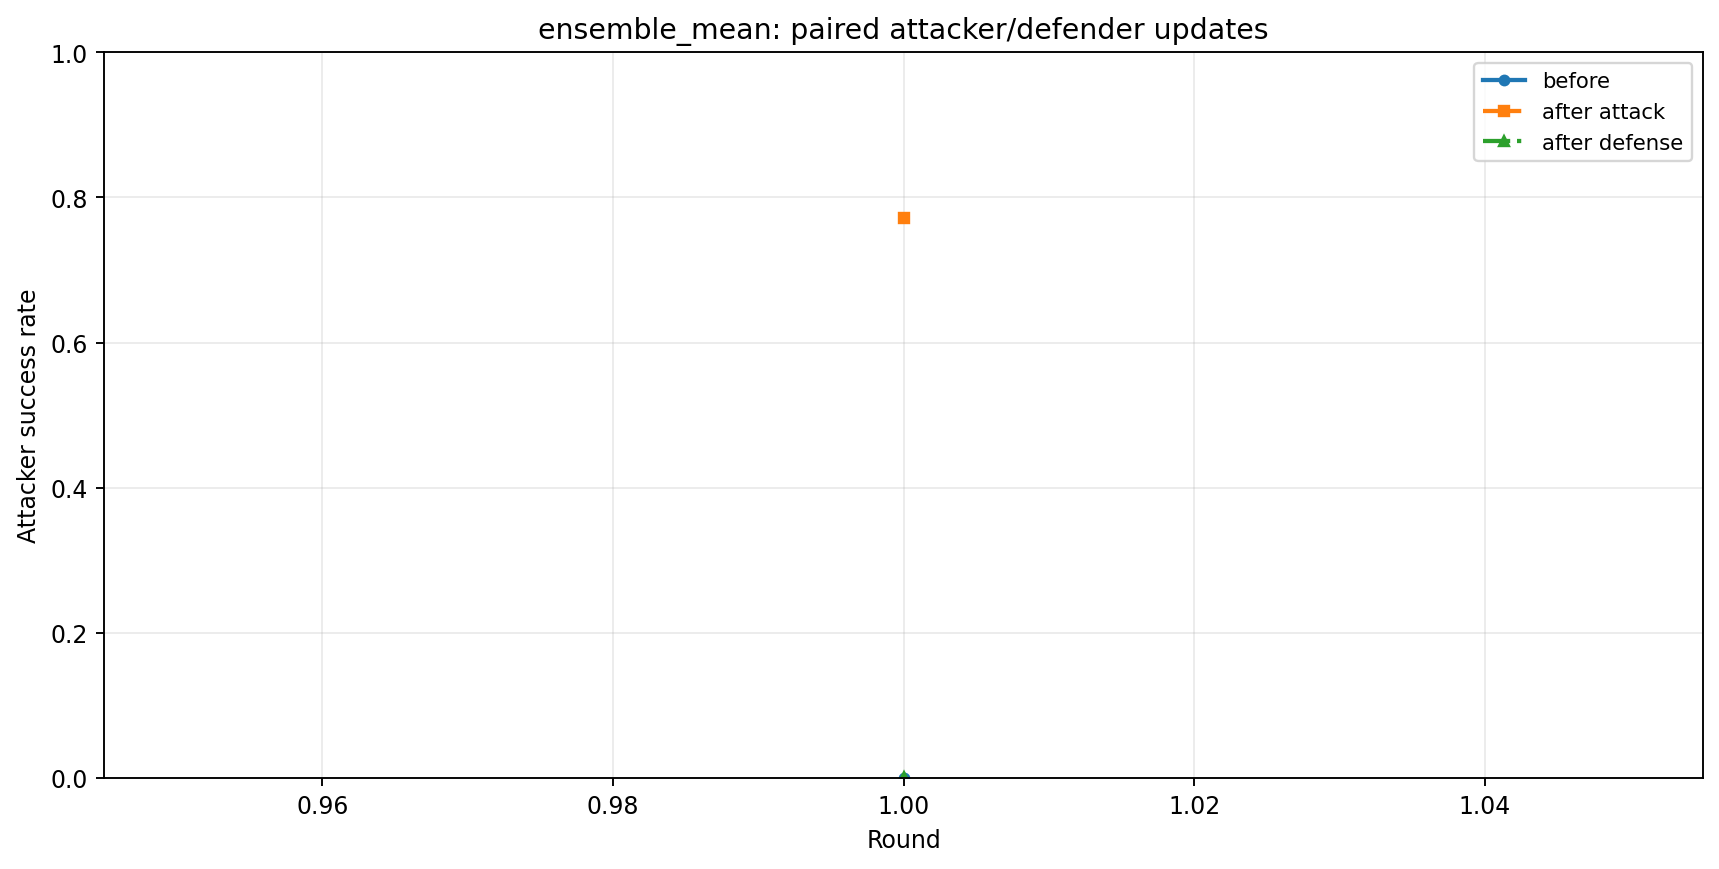
\includegraphics[keepaspectratio,alt={The after-attack and after-defense measurements reuse identical generated texts.}]{../docs/figures/research/race100-20261022T135029612516Z-gemma-ensemble_mean.png}}
\caption{The after-attack and after-defense measurements reuse identical
generated texts.}
\end{recordfigure}

The after-attack and after-defense measurements reuse identical
generated texts.
\href{../docs/figures/research/race100-20261022T135029612516Z-gemma-ensemble_mean.csv}{Source
CSV} ·
\href{../docs/figures/research/race100-20261022T135029612516Z-gemma-ensemble_mean.svg}{Vector
SVG}

Round-one checkpoint reuse: Retained attacker; begin with its first
defender update.

These are single-seed results. Successful warm-up and robustness must be
assessed from the measurements; neither is guaranteed by the training
procedure.

{\scriptsize\setlength{\tabcolsep}{3pt}\def\LTcaptype{none} % do not increment counter
\begin{longtable}[]{@{}
  >{\raggedright\arraybackslash}p{(\linewidth - 10\tabcolsep) * \real{0.1667}}
  >{\raggedright\arraybackslash}p{(\linewidth - 10\tabcolsep) * \real{0.1667}}
  >{\raggedright\arraybackslash}p{(\linewidth - 10\tabcolsep) * \real{0.1667}}
  >{\raggedright\arraybackslash}p{(\linewidth - 10\tabcolsep) * \real{0.1667}}
  >{\raggedright\arraybackslash}p{(\linewidth - 10\tabcolsep) * \real{0.1667}}
  >{\raggedright\arraybackslash}p{(\linewidth - 10\tabcolsep) * \real{0.1667}}@{}}
\toprule\noalign{}
\begin{minipage}[b]{\linewidth}\raggedright
round
\end{minipage} & \begin{minipage}[b]{\linewidth}\raggedright
phase
\end{minipage} & \begin{minipage}[b]{\linewidth}\raggedright
detector
\end{minipage} & \begin{minipage}[b]{\linewidth}\raggedright
attack\_\allowbreak{}success\_\allowbreak{}rate
\end{minipage} & \begin{minipage}[b]{\linewidth}\raggedright
ai\_\allowbreak{}detection\_\allowbreak{}rate
\end{minipage} & \begin{minipage}[b]{\linewidth}\raggedright
human\_\allowbreak{}false\_\allowbreak{}positive\_\allowbreak{}rate
\end{minipage} \\
\midrule\noalign{}
\endhead
\bottomrule\noalign{}
\endlastfoot
1 & before & decoder\_\allowbreak{}classifier & 0.0000 & 1.0000 &
0.0000 \\
1 & after\_\allowbreak{}attack & decoder\_\allowbreak{}classifier &
0.7720 & 0.2280 & 0.0000 \\
1 & after\_\allowbreak{}defense & decoder\_\allowbreak{}classifier &
0.0020 & 0.9980 & 0.0020 \\
\end{longtable}
}

{\scriptsize\setlength{\tabcolsep}{3pt}\def\LTcaptype{none} % do not increment counter
\begin{longtable}[]{@{}
  >{\raggedright\arraybackslash}p{(\linewidth - 10\tabcolsep) * \real{0.1667}}
  >{\raggedright\arraybackslash}p{(\linewidth - 10\tabcolsep) * \real{0.1667}}
  >{\raggedright\arraybackslash}p{(\linewidth - 10\tabcolsep) * \real{0.1667}}
  >{\raggedright\arraybackslash}p{(\linewidth - 10\tabcolsep) * \real{0.1667}}
  >{\raggedright\arraybackslash}p{(\linewidth - 10\tabcolsep) * \real{0.1667}}
  >{\raggedright\arraybackslash}p{(\linewidth - 10\tabcolsep) * \real{0.1667}}@{}}
\toprule\noalign{}
\begin{minipage}[b]{\linewidth}\raggedright
round
\end{minipage} & \begin{minipage}[b]{\linewidth}\raggedright
phase
\end{minipage} & \begin{minipage}[b]{\linewidth}\raggedright
detector
\end{minipage} & \begin{minipage}[b]{\linewidth}\raggedright
roc\_\allowbreak{}auc
\end{minipage} & \begin{minipage}[b]{\linewidth}\raggedright
semantic\_\allowbreak{}similarity
\end{minipage} & \begin{minipage}[b]{\linewidth}\raggedright
num\_\allowbreak{}generated
\end{minipage} \\
\midrule\noalign{}
\endhead
\bottomrule\noalign{}
\endlastfoot
1 & before & decoder\_\allowbreak{}classifier & 1.0000 & undefined &
500 \\
1 & after\_\allowbreak{}attack & decoder\_\allowbreak{}classifier &
0.9124 & 0.8867 & 500 \\
1 & after\_\allowbreak{}defense & decoder\_\allowbreak{}classifier &
1.0000 & 0.8867 & 500 \\
\end{longtable}
}

{\scriptsize\setlength{\tabcolsep}{3pt}\def\LTcaptype{none} % do not increment counter
\begin{longtable}[]{@{}
  >{\raggedright\arraybackslash}p{(\linewidth - 6\tabcolsep) * \real{0.2500}}
  >{\raggedright\arraybackslash}p{(\linewidth - 6\tabcolsep) * \real{0.2500}}
  >{\raggedright\arraybackslash}p{(\linewidth - 6\tabcolsep) * \real{0.2500}}
  >{\raggedright\arraybackslash}p{(\linewidth - 6\tabcolsep) * \real{0.2500}}@{}}
\toprule\noalign{}
\begin{minipage}[b]{\linewidth}\raggedright
round
\end{minipage} & \begin{minipage}[b]{\linewidth}\raggedright
phase
\end{minipage} & \begin{minipage}[b]{\linewidth}\raggedright
detector
\end{minipage} & \begin{minipage}[b]{\linewidth}\raggedright
num\_\allowbreak{}ineligible\_\allowbreak{}pairs
\end{minipage} \\
\midrule\noalign{}
\endhead
\bottomrule\noalign{}
\endlastfoot
1 & before & decoder\_\allowbreak{}classifier & 0 \\
1 & after\_\allowbreak{}attack & decoder\_\allowbreak{}classifier & 0 \\
1 & after\_\allowbreak{}defense & decoder\_\allowbreak{}classifier &
0 \\
\end{longtable}
}

\subsubsection{modernbert: job
1447845}\label{record-docs-research-results-md-modernbert-job-1447845}

Status: completed; completed rounds: 1/1.

Retained attacker:
\texttt{\seqsplit{/lustre/fswork/projects/rech/mbm/ual37ci/bench\_research\_ml\_project/split-repos/ai-content-robustness/results/research\_workflow/defender\_comparison/rl/encoder/checkpoint-1487}},
trained for \textbf{1487 updates}. Initial evaluations reuse the saved
texts and scores after identity checks. Post-defense evaluation reuses
exactly those attack texts.

{\scriptsize\setlength{\tabcolsep}{3pt}\def\LTcaptype{none} % do not increment counter
\begin{longtable}[]{@{}
  >{\raggedright\arraybackslash}p{(\linewidth - 8\tabcolsep) * \real{0.2000}}
  >{\raggedright\arraybackslash}p{(\linewidth - 8\tabcolsep) * \real{0.2000}}
  >{\raggedright\arraybackslash}p{(\linewidth - 8\tabcolsep) * \real{0.2000}}
  >{\raggedright\arraybackslash}p{(\linewidth - 8\tabcolsep) * \real{0.2000}}
  >{\raggedright\arraybackslash}p{(\linewidth - 8\tabcolsep) * \real{0.2000}}@{}}
\toprule\noalign{}
\begin{minipage}[b]{\linewidth}\raggedright
round
\end{minipage} & \begin{minipage}[b]{\linewidth}\raggedright
detector
\end{minipage} & \begin{minipage}[b]{\linewidth}\raggedright
before
\end{minipage} & \begin{minipage}[b]{\linewidth}\raggedright
after\_\allowbreak{}attack
\end{minipage} & \begin{minipage}[b]{\linewidth}\raggedright
after\_\allowbreak{}defense
\end{minipage} \\
\midrule\noalign{}
\endhead
\bottomrule\noalign{}
\endlastfoot
1 & modernbert\_\allowbreak{}large & 0.0100 & 0.9680 & 0.0100 \\
1 & ensemble\_\allowbreak{}mean & 0.0100 & 0.9680 & 0.0100 \\
\end{longtable}
}

\begin{recordfigure}
\centering
\pandocbounded{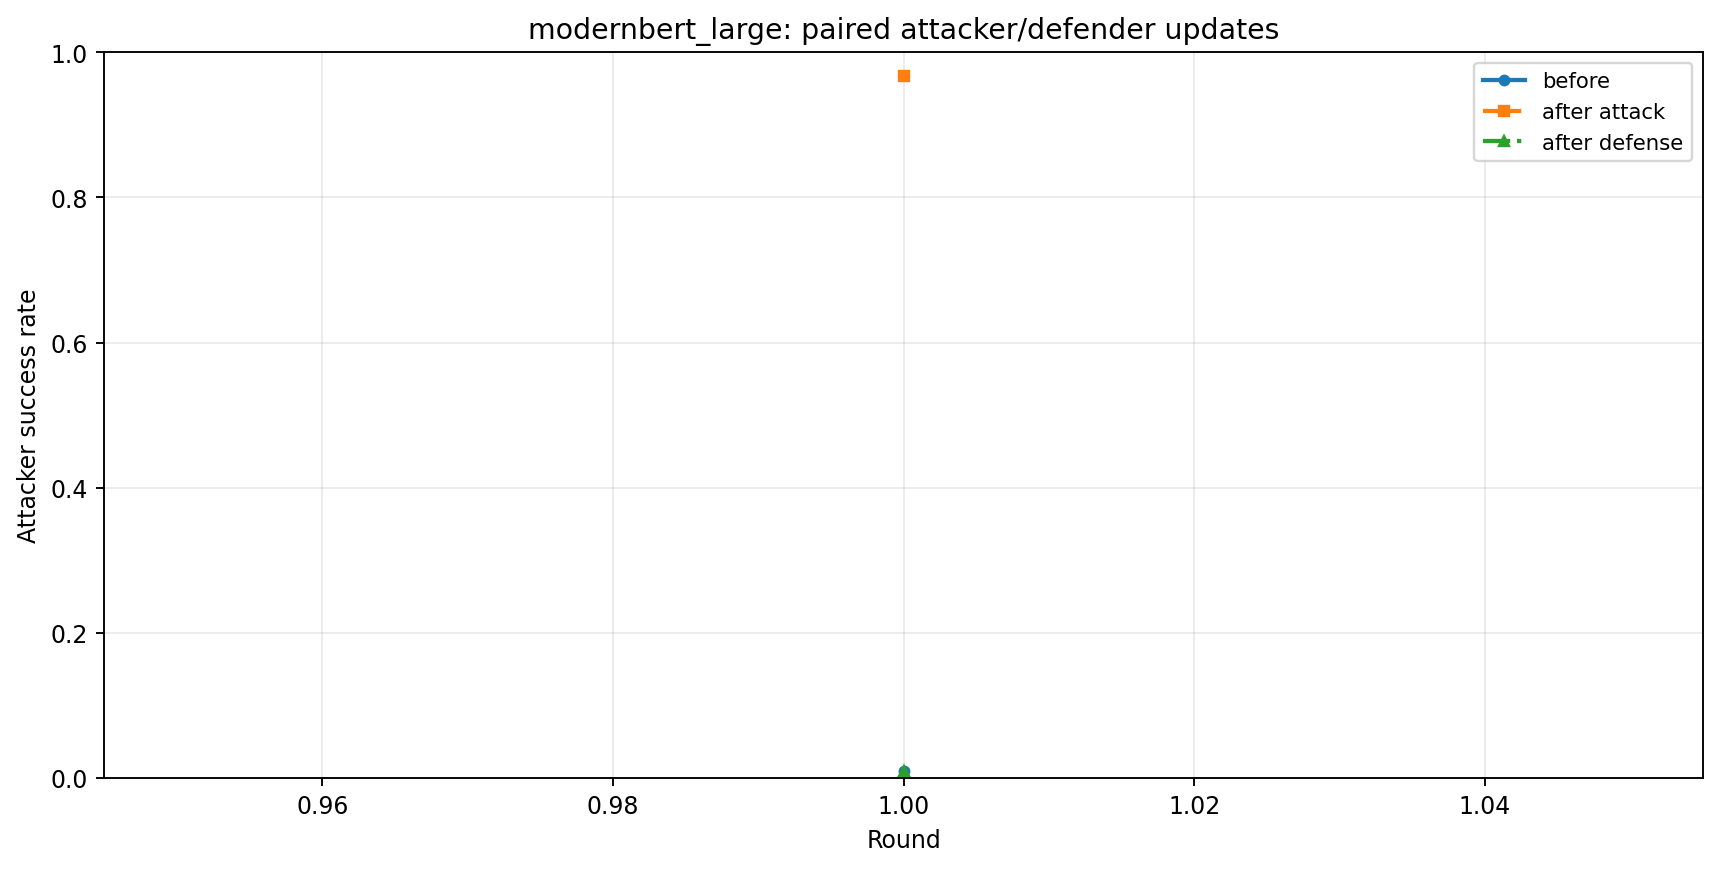
\includegraphics[keepaspectratio,alt={The after-attack and after-defense measurements reuse identical generated texts.}]{../docs/figures/research/race100-20261022T135029612516Z-modernbert-modernbert_large.png}}
\caption{The after-attack and after-defense measurements reuse identical
generated texts.}
\end{recordfigure}

The after-attack and after-defense measurements reuse identical
generated texts.
\href{../docs/figures/research/race100-20261022T135029612516Z-modernbert-modernbert_large.csv}{Source
CSV} ·
\href{../docs/figures/research/race100-20261022T135029612516Z-modernbert-modernbert_large.svg}{Vector
SVG}

\begin{recordfigure}
\centering
\pandocbounded{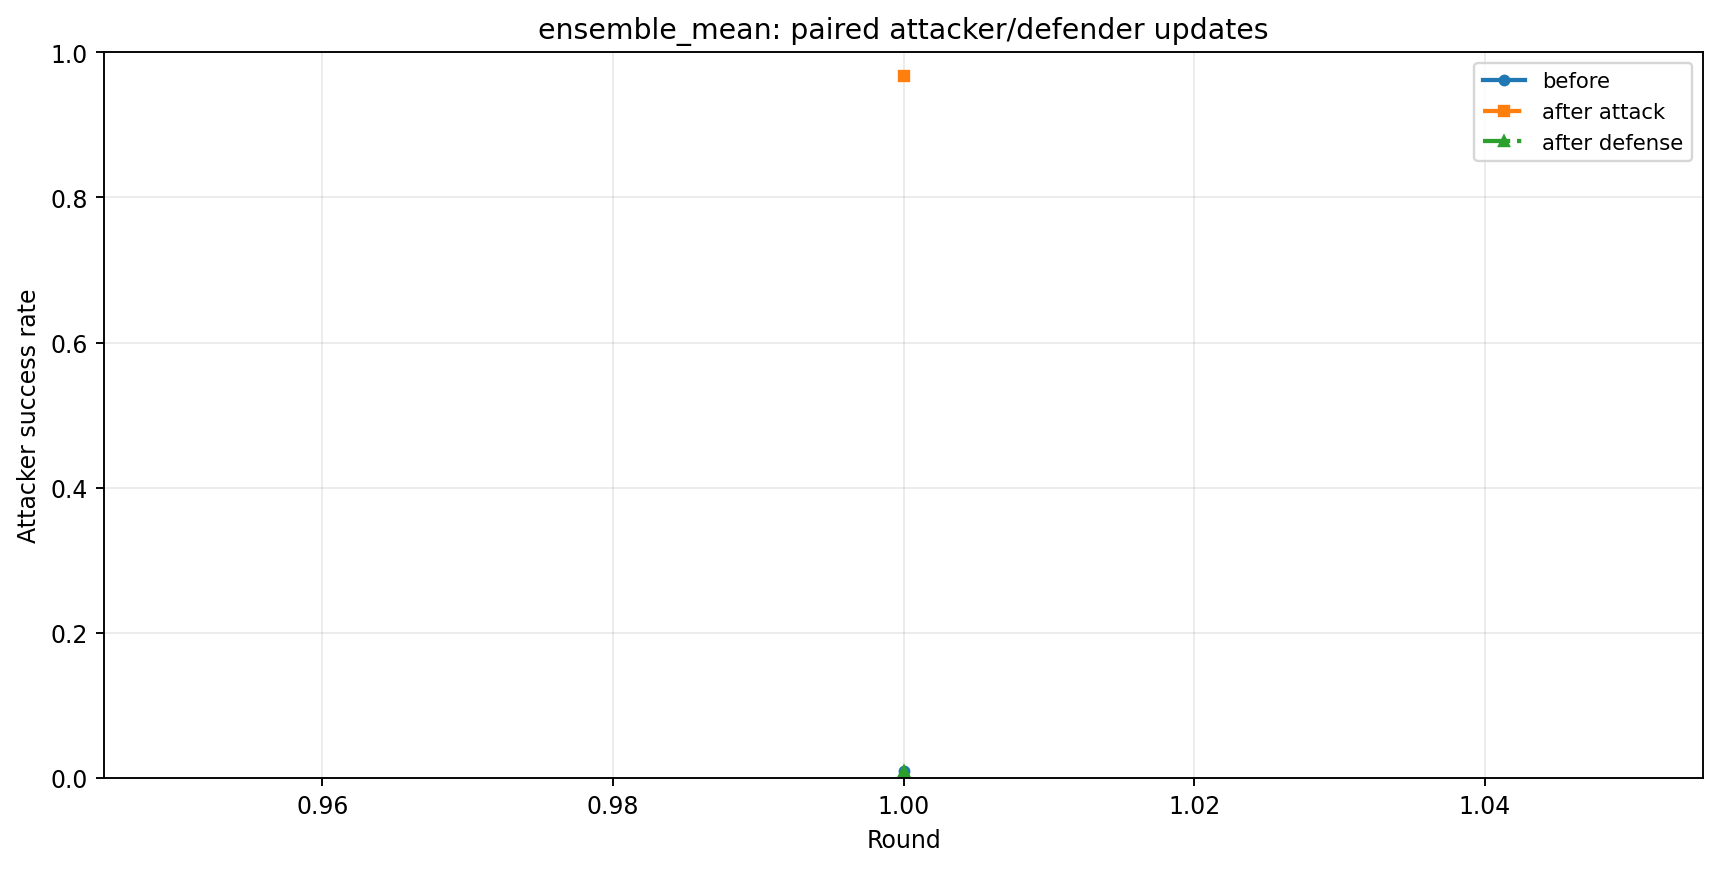
\includegraphics[keepaspectratio,alt={The after-attack and after-defense measurements reuse identical generated texts.}]{../docs/figures/research/race100-20261022T135029612516Z-modernbert-ensemble_mean.png}}
\caption{The after-attack and after-defense measurements reuse identical
generated texts.}
\end{recordfigure}

The after-attack and after-defense measurements reuse identical
generated texts.
\href{../docs/figures/research/race100-20261022T135029612516Z-modernbert-ensemble_mean.csv}{Source
CSV} ·
\href{../docs/figures/research/race100-20261022T135029612516Z-modernbert-ensemble_mean.svg}{Vector
SVG}

Round-one checkpoint reuse: Retained attacker; begin with its first
defender update.

These are single-seed results. Successful warm-up and robustness must be
assessed from the measurements; neither is guaranteed by the training
procedure.

{\scriptsize\setlength{\tabcolsep}{3pt}\def\LTcaptype{none} % do not increment counter
\begin{longtable}[]{@{}
  >{\raggedright\arraybackslash}p{(\linewidth - 10\tabcolsep) * \real{0.1667}}
  >{\raggedright\arraybackslash}p{(\linewidth - 10\tabcolsep) * \real{0.1667}}
  >{\raggedright\arraybackslash}p{(\linewidth - 10\tabcolsep) * \real{0.1667}}
  >{\raggedright\arraybackslash}p{(\linewidth - 10\tabcolsep) * \real{0.1667}}
  >{\raggedright\arraybackslash}p{(\linewidth - 10\tabcolsep) * \real{0.1667}}
  >{\raggedright\arraybackslash}p{(\linewidth - 10\tabcolsep) * \real{0.1667}}@{}}
\toprule\noalign{}
\begin{minipage}[b]{\linewidth}\raggedright
round
\end{minipage} & \begin{minipage}[b]{\linewidth}\raggedright
phase
\end{minipage} & \begin{minipage}[b]{\linewidth}\raggedright
detector
\end{minipage} & \begin{minipage}[b]{\linewidth}\raggedright
attack\_\allowbreak{}success\_\allowbreak{}rate
\end{minipage} & \begin{minipage}[b]{\linewidth}\raggedright
ai\_\allowbreak{}detection\_\allowbreak{}rate
\end{minipage} & \begin{minipage}[b]{\linewidth}\raggedright
human\_\allowbreak{}false\_\allowbreak{}positive\_\allowbreak{}rate
\end{minipage} \\
\midrule\noalign{}
\endhead
\bottomrule\noalign{}
\endlastfoot
1 & before & modernbert\_\allowbreak{}large & 0.0100 & 0.9900 &
0.0160 \\
1 & after\_\allowbreak{}attack & modernbert\_\allowbreak{}large & 0.9680
& 0.0320 & 0.0160 \\
1 & after\_\allowbreak{}defense & modernbert\_\allowbreak{}large &
0.0100 & 0.9900 & 0.0040 \\
\end{longtable}
}

{\scriptsize\setlength{\tabcolsep}{3pt}\def\LTcaptype{none} % do not increment counter
\begin{longtable}[]{@{}
  >{\raggedright\arraybackslash}p{(\linewidth - 10\tabcolsep) * \real{0.1667}}
  >{\raggedright\arraybackslash}p{(\linewidth - 10\tabcolsep) * \real{0.1667}}
  >{\raggedright\arraybackslash}p{(\linewidth - 10\tabcolsep) * \real{0.1667}}
  >{\raggedright\arraybackslash}p{(\linewidth - 10\tabcolsep) * \real{0.1667}}
  >{\raggedright\arraybackslash}p{(\linewidth - 10\tabcolsep) * \real{0.1667}}
  >{\raggedright\arraybackslash}p{(\linewidth - 10\tabcolsep) * \real{0.1667}}@{}}
\toprule\noalign{}
\begin{minipage}[b]{\linewidth}\raggedright
round
\end{minipage} & \begin{minipage}[b]{\linewidth}\raggedright
phase
\end{minipage} & \begin{minipage}[b]{\linewidth}\raggedright
detector
\end{minipage} & \begin{minipage}[b]{\linewidth}\raggedright
roc\_\allowbreak{}auc
\end{minipage} & \begin{minipage}[b]{\linewidth}\raggedright
semantic\_\allowbreak{}similarity
\end{minipage} & \begin{minipage}[b]{\linewidth}\raggedright
num\_\allowbreak{}generated
\end{minipage} \\
\midrule\noalign{}
\endhead
\bottomrule\noalign{}
\endlastfoot
1 & before & modernbert\_\allowbreak{}large & 0.9992 & undefined &
500 \\
1 & after\_\allowbreak{}attack & modernbert\_\allowbreak{}large & 0.7104
& 0.8821 & 500 \\
1 & after\_\allowbreak{}defense & modernbert\_\allowbreak{}large &
0.9998 & 0.8821 & 500 \\
\end{longtable}
}

{\scriptsize\setlength{\tabcolsep}{3pt}\def\LTcaptype{none} % do not increment counter
\begin{longtable}[]{@{}
  >{\raggedright\arraybackslash}p{(\linewidth - 6\tabcolsep) * \real{0.2500}}
  >{\raggedright\arraybackslash}p{(\linewidth - 6\tabcolsep) * \real{0.2500}}
  >{\raggedright\arraybackslash}p{(\linewidth - 6\tabcolsep) * \real{0.2500}}
  >{\raggedright\arraybackslash}p{(\linewidth - 6\tabcolsep) * \real{0.2500}}@{}}
\toprule\noalign{}
\begin{minipage}[b]{\linewidth}\raggedright
round
\end{minipage} & \begin{minipage}[b]{\linewidth}\raggedright
phase
\end{minipage} & \begin{minipage}[b]{\linewidth}\raggedright
detector
\end{minipage} & \begin{minipage}[b]{\linewidth}\raggedright
num\_\allowbreak{}ineligible\_\allowbreak{}pairs
\end{minipage} \\
\midrule\noalign{}
\endhead
\bottomrule\noalign{}
\endlastfoot
1 & before & modernbert\_\allowbreak{}large & 0 \\
1 & after\_\allowbreak{}attack & modernbert\_\allowbreak{}large & 0 \\
1 & after\_\allowbreak{}defense & modernbert\_\allowbreak{}large & 0 \\
\end{longtable}
}

\subsubsection{ensemble: job
1447846}\label{record-docs-research-results-md-ensemble-job-1447846}

Status: completed; completed rounds: 1/1.

Retained attacker:
\texttt{\seqsplit{/lustre/fswork/projects/rech/mbm/ual37ci/bench\_research\_ml\_project/split-repos/ai-content-robustness/results/research\_workflow/defender\_comparison/rl/ensemble/checkpoint-502}},
trained for \textbf{502 updates}. Initial evaluations reuse the saved
texts and scores after identity checks. Post-defense evaluation reuses
exactly those attack texts.

{\scriptsize\setlength{\tabcolsep}{3pt}\def\LTcaptype{none} % do not increment counter
\begin{longtable}[]{@{}
  >{\raggedright\arraybackslash}p{(\linewidth - 8\tabcolsep) * \real{0.2000}}
  >{\raggedright\arraybackslash}p{(\linewidth - 8\tabcolsep) * \real{0.2000}}
  >{\raggedright\arraybackslash}p{(\linewidth - 8\tabcolsep) * \real{0.2000}}
  >{\raggedright\arraybackslash}p{(\linewidth - 8\tabcolsep) * \real{0.2000}}
  >{\raggedright\arraybackslash}p{(\linewidth - 8\tabcolsep) * \real{0.2000}}@{}}
\toprule\noalign{}
\begin{minipage}[b]{\linewidth}\raggedright
round
\end{minipage} & \begin{minipage}[b]{\linewidth}\raggedright
detector
\end{minipage} & \begin{minipage}[b]{\linewidth}\raggedright
before
\end{minipage} & \begin{minipage}[b]{\linewidth}\raggedright
after\_\allowbreak{}attack
\end{minipage} & \begin{minipage}[b]{\linewidth}\raggedright
after\_\allowbreak{}defense
\end{minipage} \\
\midrule\noalign{}
\endhead
\bottomrule\noalign{}
\endlastfoot
1 & binoculars & 0.0140 & 0.9400 & 0.0060 \\
1 & fast\_\allowbreak{}detect\_\allowbreak{}gpt & 0.0000 & 0.9300 &
0.0000 \\
1 & diveye & 0.0280 & 0.8100 & 0.0700 \\
1 & roberta & 0.0000 & 0.9220 & 0.0080 \\
1 & tfidf & 0.1140 & 0.9660 & 0.0580 \\
1 & modernbert\_\allowbreak{}large & 0.0100 & 0.9800 & 0.0080 \\
1 & decoder\_\allowbreak{}classifier & 0.0000 & 0.7700 & 0.0020 \\
1 & ensemble\_\allowbreak{}mean & 0.0000 & 0.9480 & 0.0040 \\
\end{longtable}
}

\begin{recordfigure}
\centering
\pandocbounded{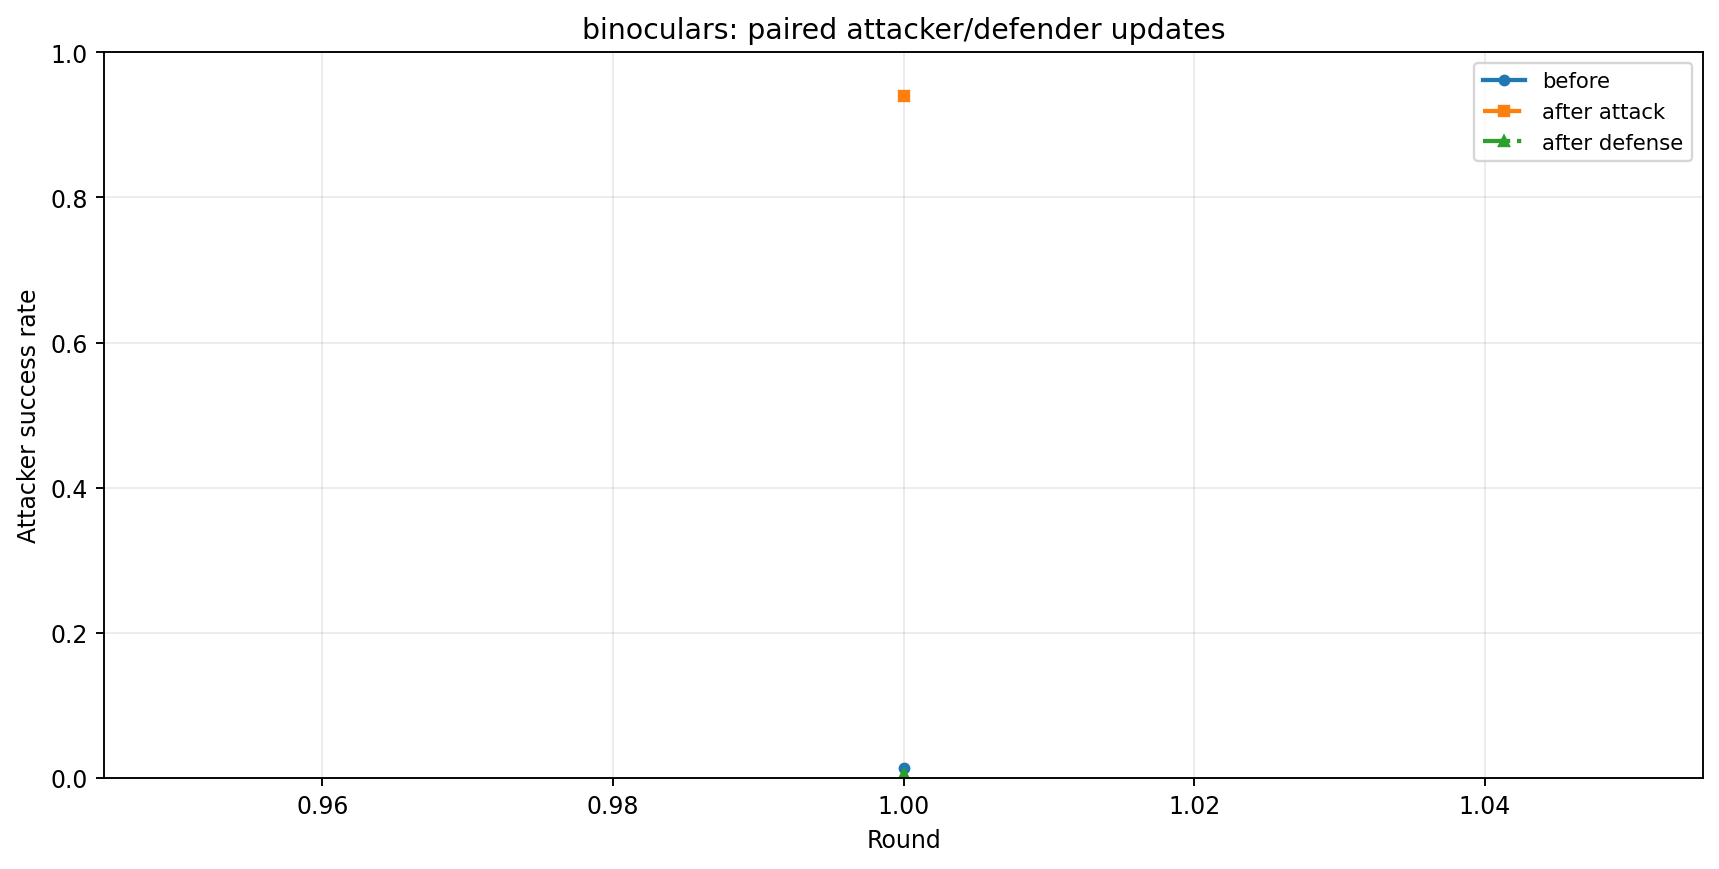
\includegraphics[keepaspectratio,alt={The after-attack and after-defense measurements reuse identical generated texts.}]{../docs/figures/research/race100-20261022T135029612516Z-ensemble-binoculars.png}}
\caption{The after-attack and after-defense measurements reuse identical
generated texts.}
\end{recordfigure}

The after-attack and after-defense measurements reuse identical
generated texts.
\href{../docs/figures/research/race100-20261022T135029612516Z-ensemble-binoculars.csv}{Source
CSV} ·
\href{../docs/figures/research/race100-20261022T135029612516Z-ensemble-binoculars.svg}{Vector
SVG}

\begin{recordfigure}
\centering
\pandocbounded{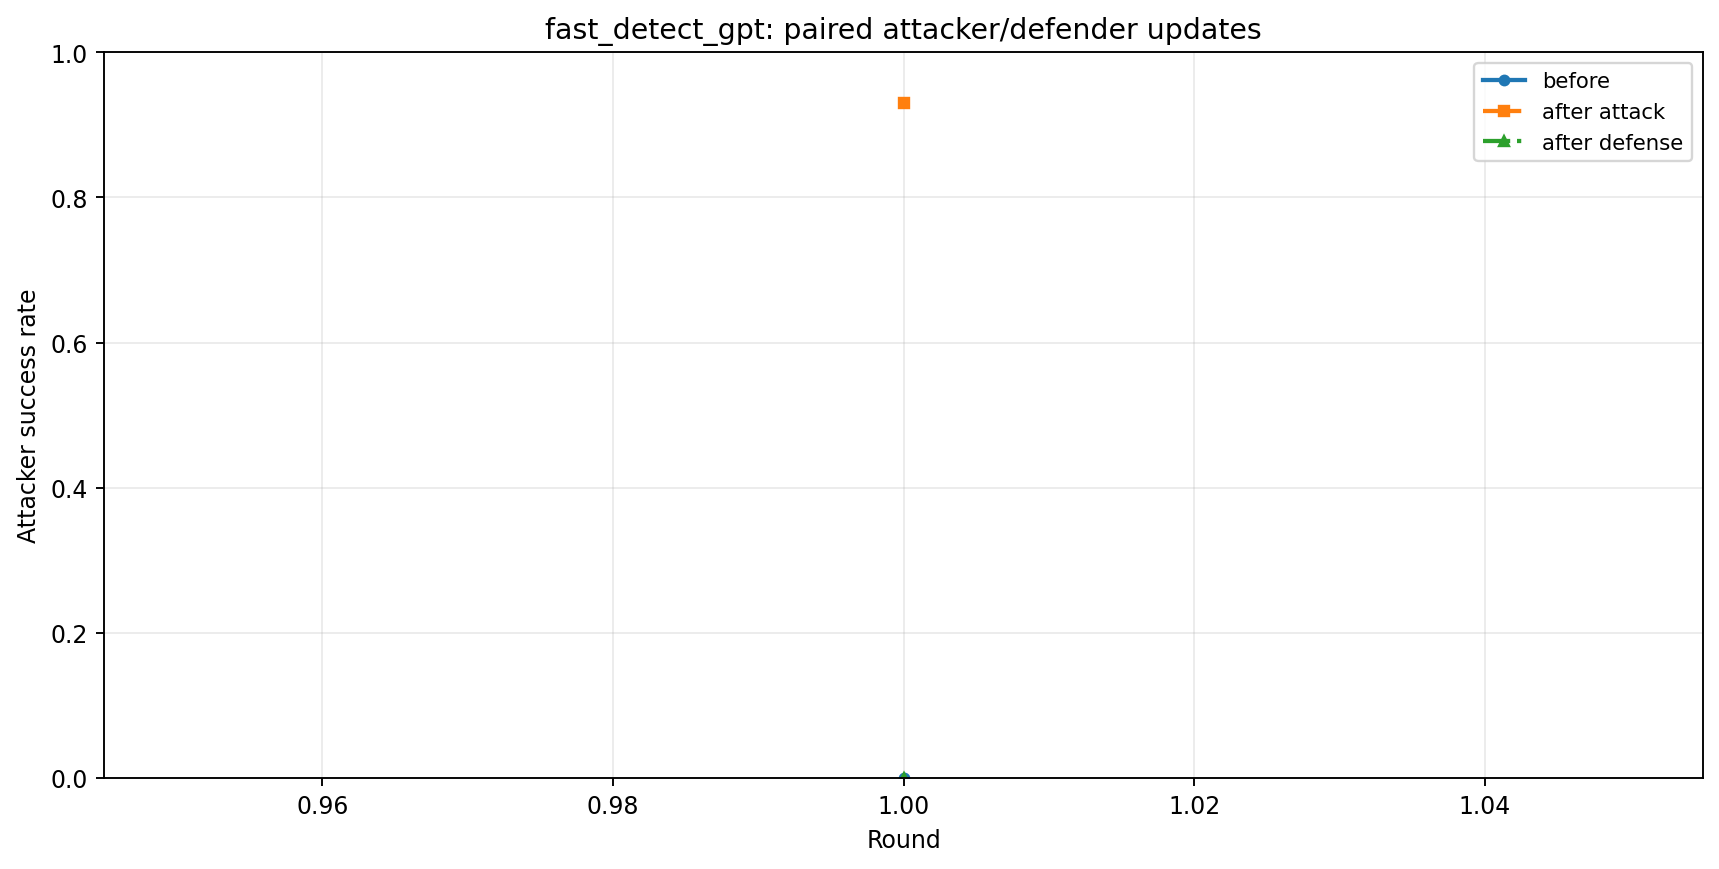
\includegraphics[keepaspectratio,alt={The after-attack and after-defense measurements reuse identical generated texts.}]{../docs/figures/research/race100-20261022T135029612516Z-ensemble-fast_detect_gpt.png}}
\caption{The after-attack and after-defense measurements reuse identical
generated texts.}
\end{recordfigure}

The after-attack and after-defense measurements reuse identical
generated texts.
\href{../docs/figures/research/race100-20261022T135029612516Z-ensemble-fast_detect_gpt.csv}{Source
CSV} ·
\href{../docs/figures/research/race100-20261022T135029612516Z-ensemble-fast_detect_gpt.svg}{Vector
SVG}

\begin{recordfigure}
\centering
\pandocbounded{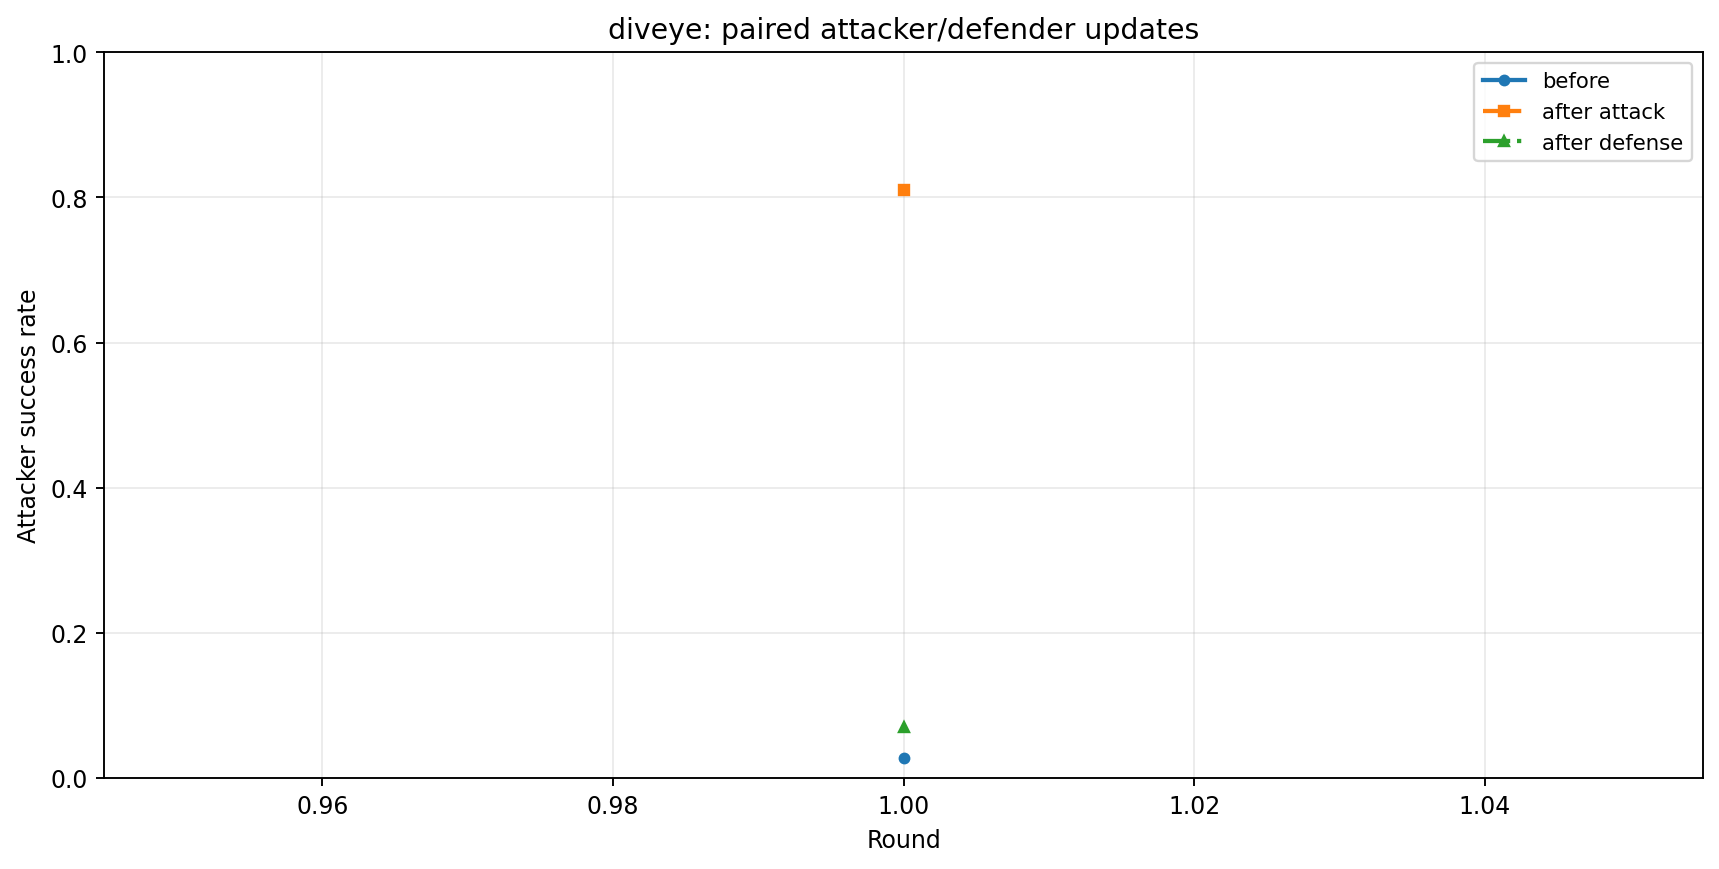
\includegraphics[keepaspectratio,alt={The after-attack and after-defense measurements reuse identical generated texts.}]{../docs/figures/research/race100-20261022T135029612516Z-ensemble-diveye.png}}
\caption{The after-attack and after-defense measurements reuse identical
generated texts.}
\end{recordfigure}

The after-attack and after-defense measurements reuse identical
generated texts.
\href{../docs/figures/research/race100-20261022T135029612516Z-ensemble-diveye.csv}{Source
CSV} ·
\href{../docs/figures/research/race100-20261022T135029612516Z-ensemble-diveye.svg}{Vector
SVG}

\begin{recordfigure}
\centering
\pandocbounded{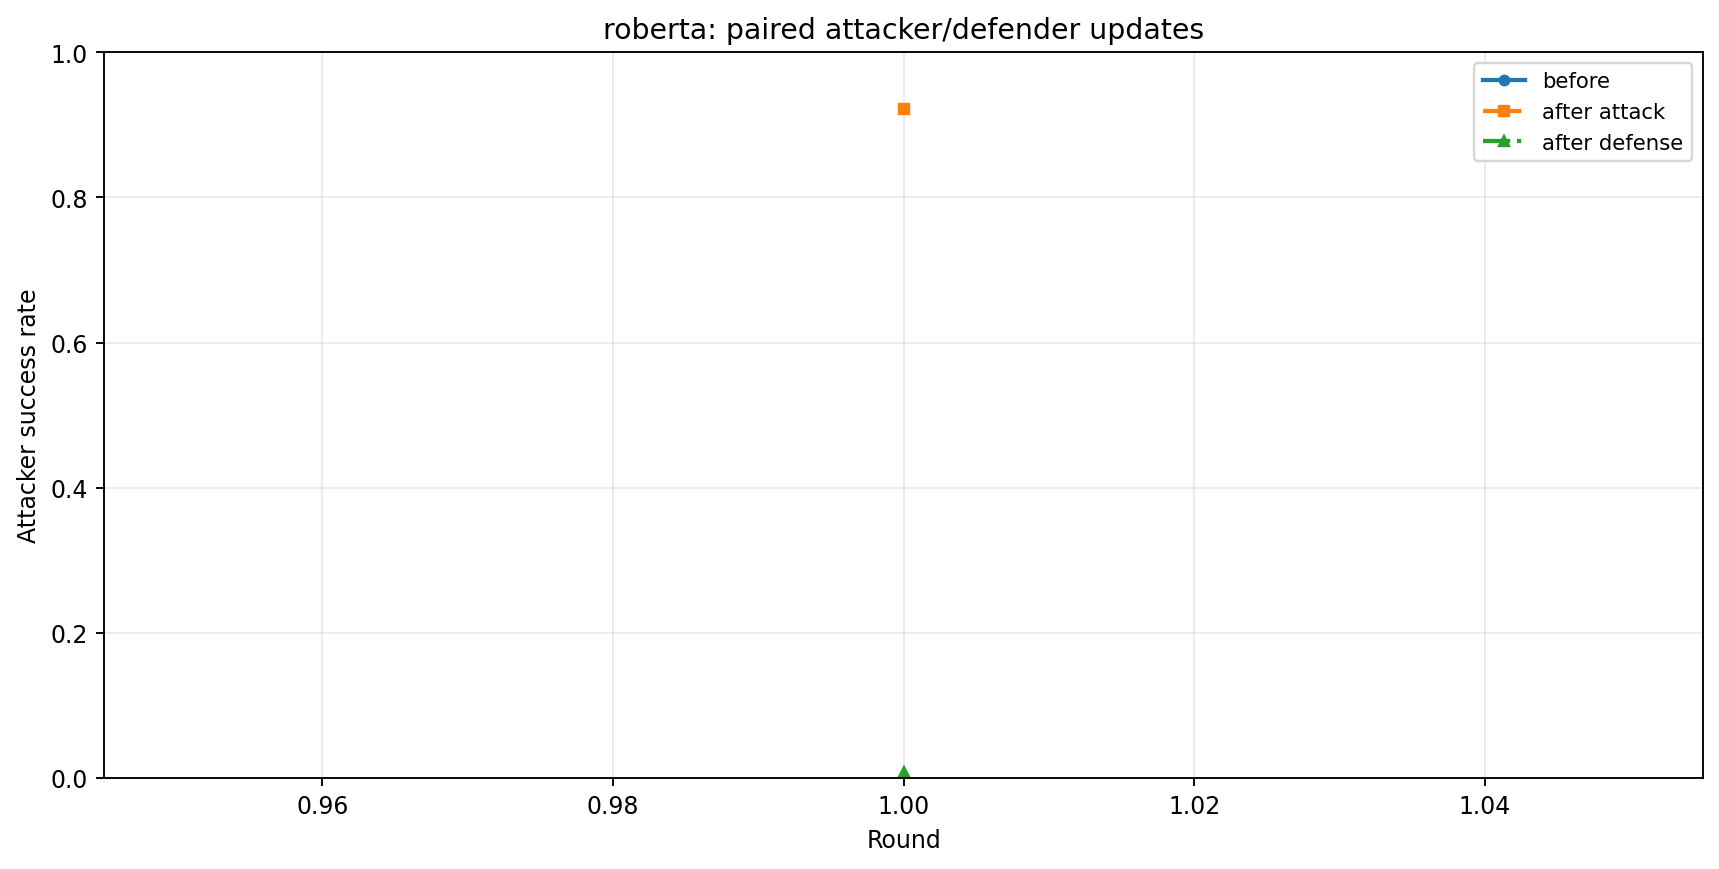
\includegraphics[keepaspectratio,alt={The after-attack and after-defense measurements reuse identical generated texts.}]{../docs/figures/research/race100-20261022T135029612516Z-ensemble-roberta.png}}
\caption{The after-attack and after-defense measurements reuse identical
generated texts.}
\end{recordfigure}

The after-attack and after-defense measurements reuse identical
generated texts.
\href{../docs/figures/research/race100-20261022T135029612516Z-ensemble-roberta.csv}{Source
CSV} ·
\href{../docs/figures/research/race100-20261022T135029612516Z-ensemble-roberta.svg}{Vector
SVG}

\begin{recordfigure}
\centering
\pandocbounded{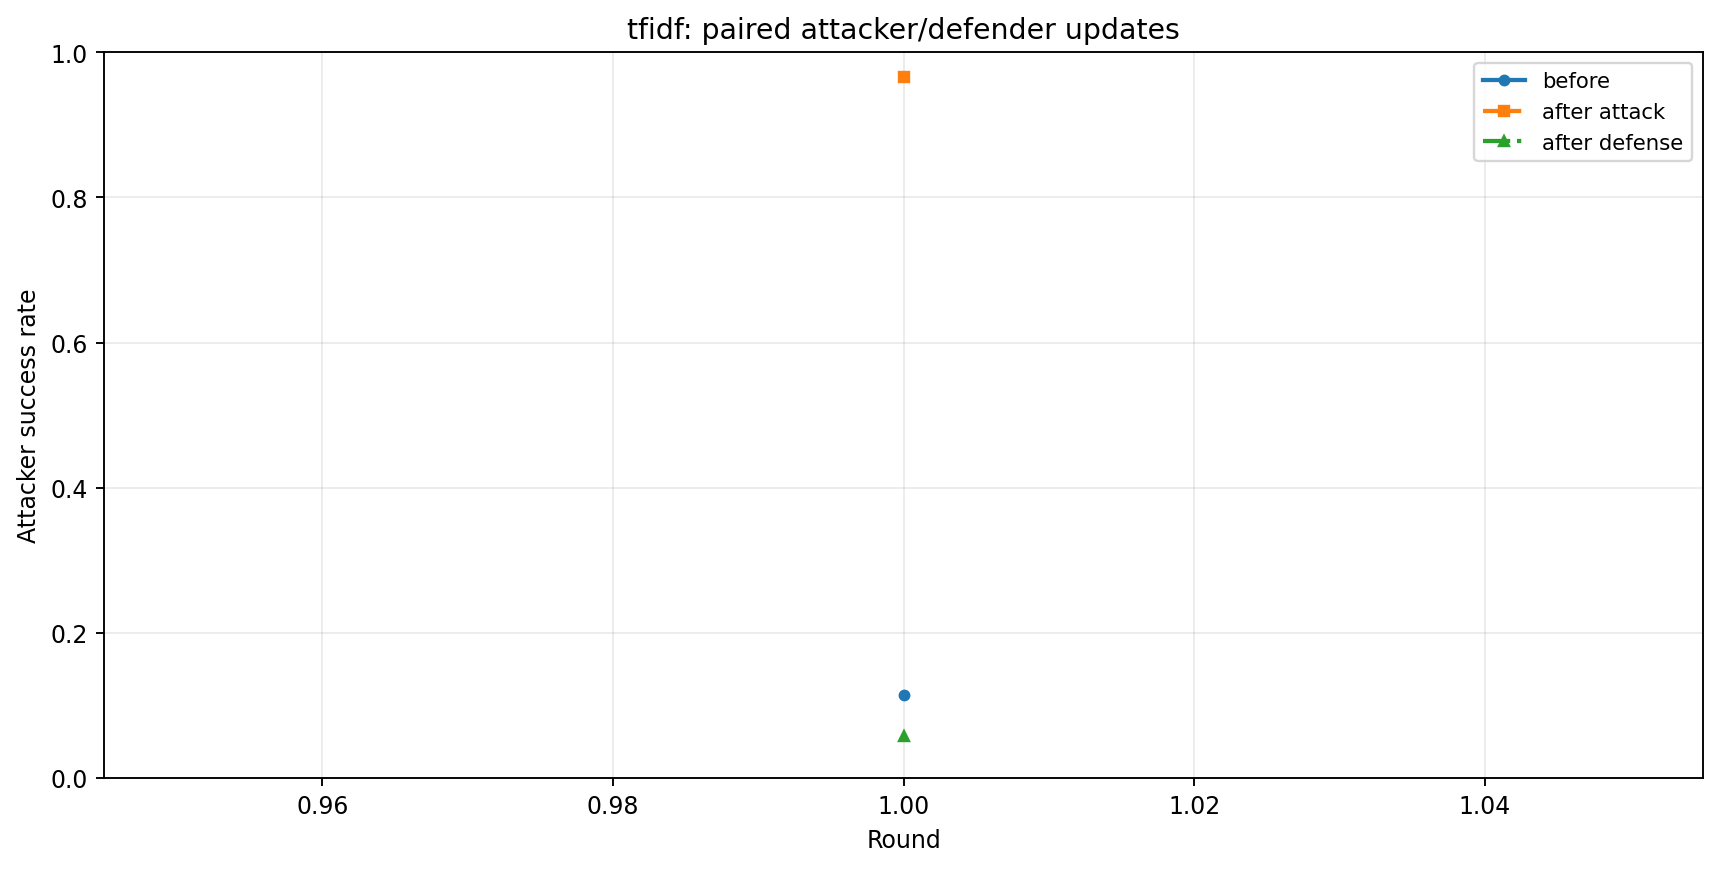
\includegraphics[keepaspectratio,alt={The after-attack and after-defense measurements reuse identical generated texts.}]{../docs/figures/research/race100-20261022T135029612516Z-ensemble-tfidf.png}}
\caption{The after-attack and after-defense measurements reuse identical
generated texts.}
\end{recordfigure}

The after-attack and after-defense measurements reuse identical
generated texts.
\href{../docs/figures/research/race100-20261022T135029612516Z-ensemble-tfidf.csv}{Source
CSV} ·
\href{../docs/figures/research/race100-20261022T135029612516Z-ensemble-tfidf.svg}{Vector
SVG}

\begin{recordfigure}
\centering
\pandocbounded{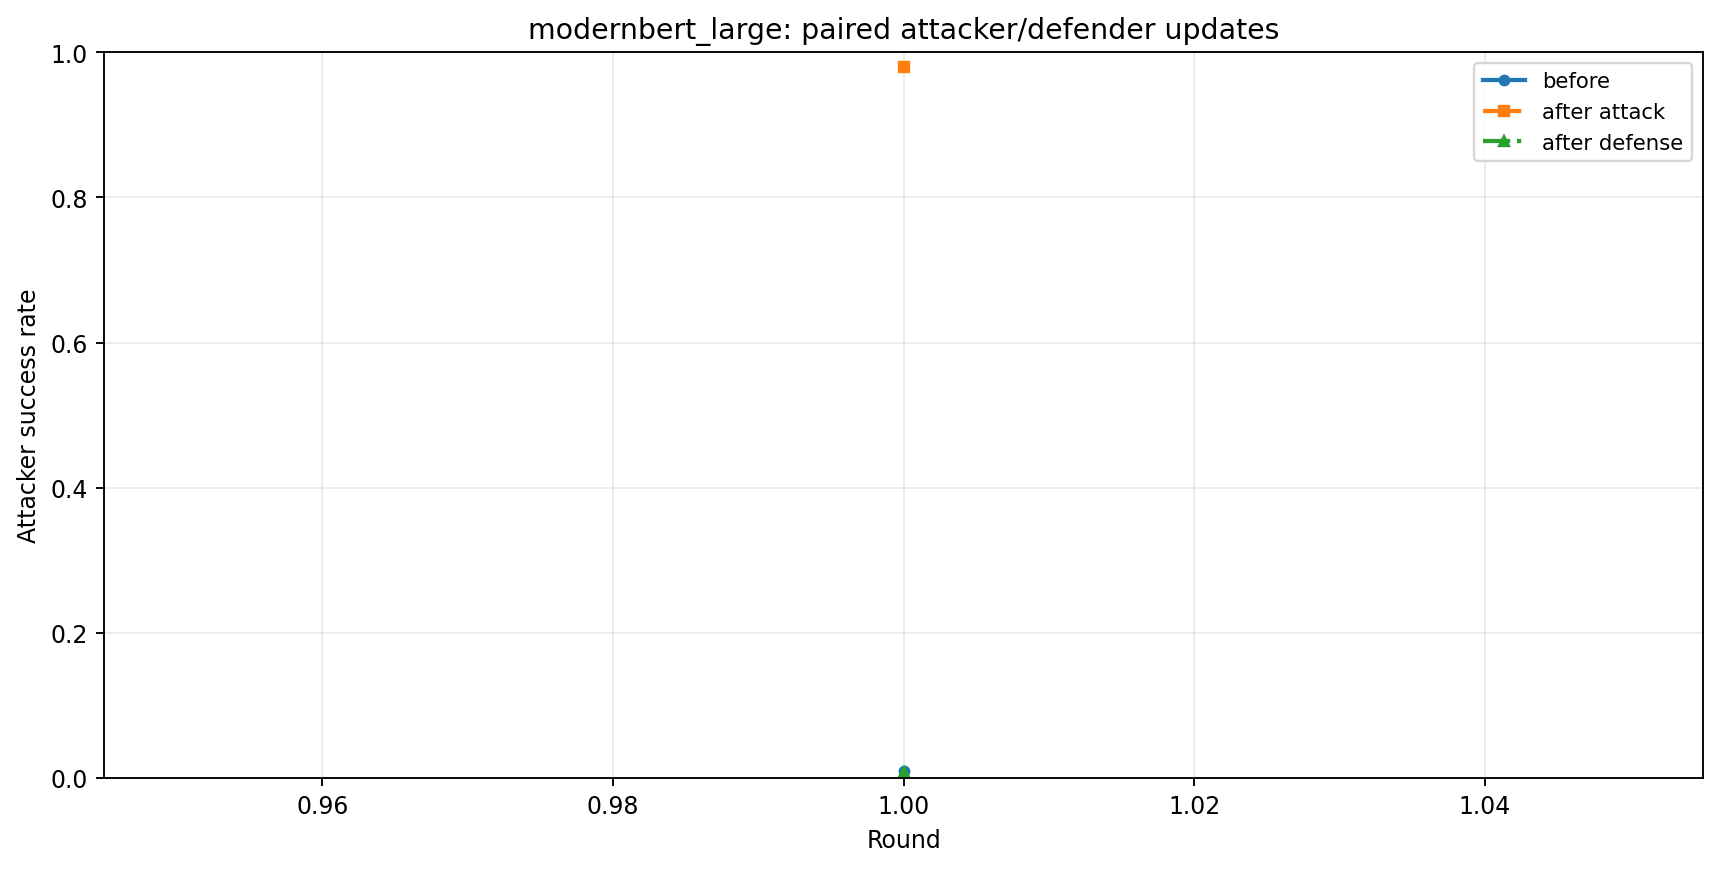
\includegraphics[keepaspectratio,alt={The after-attack and after-defense measurements reuse identical generated texts.}]{../docs/figures/research/race100-20261022T135029612516Z-ensemble-modernbert_large.png}}
\caption{The after-attack and after-defense measurements reuse identical
generated texts.}
\end{recordfigure}

The after-attack and after-defense measurements reuse identical
generated texts.
\href{../docs/figures/research/race100-20261022T135029612516Z-ensemble-modernbert_large.csv}{Source
CSV} ·
\href{../docs/figures/research/race100-20261022T135029612516Z-ensemble-modernbert_large.svg}{Vector
SVG}

\begin{recordfigure}
\centering
\pandocbounded{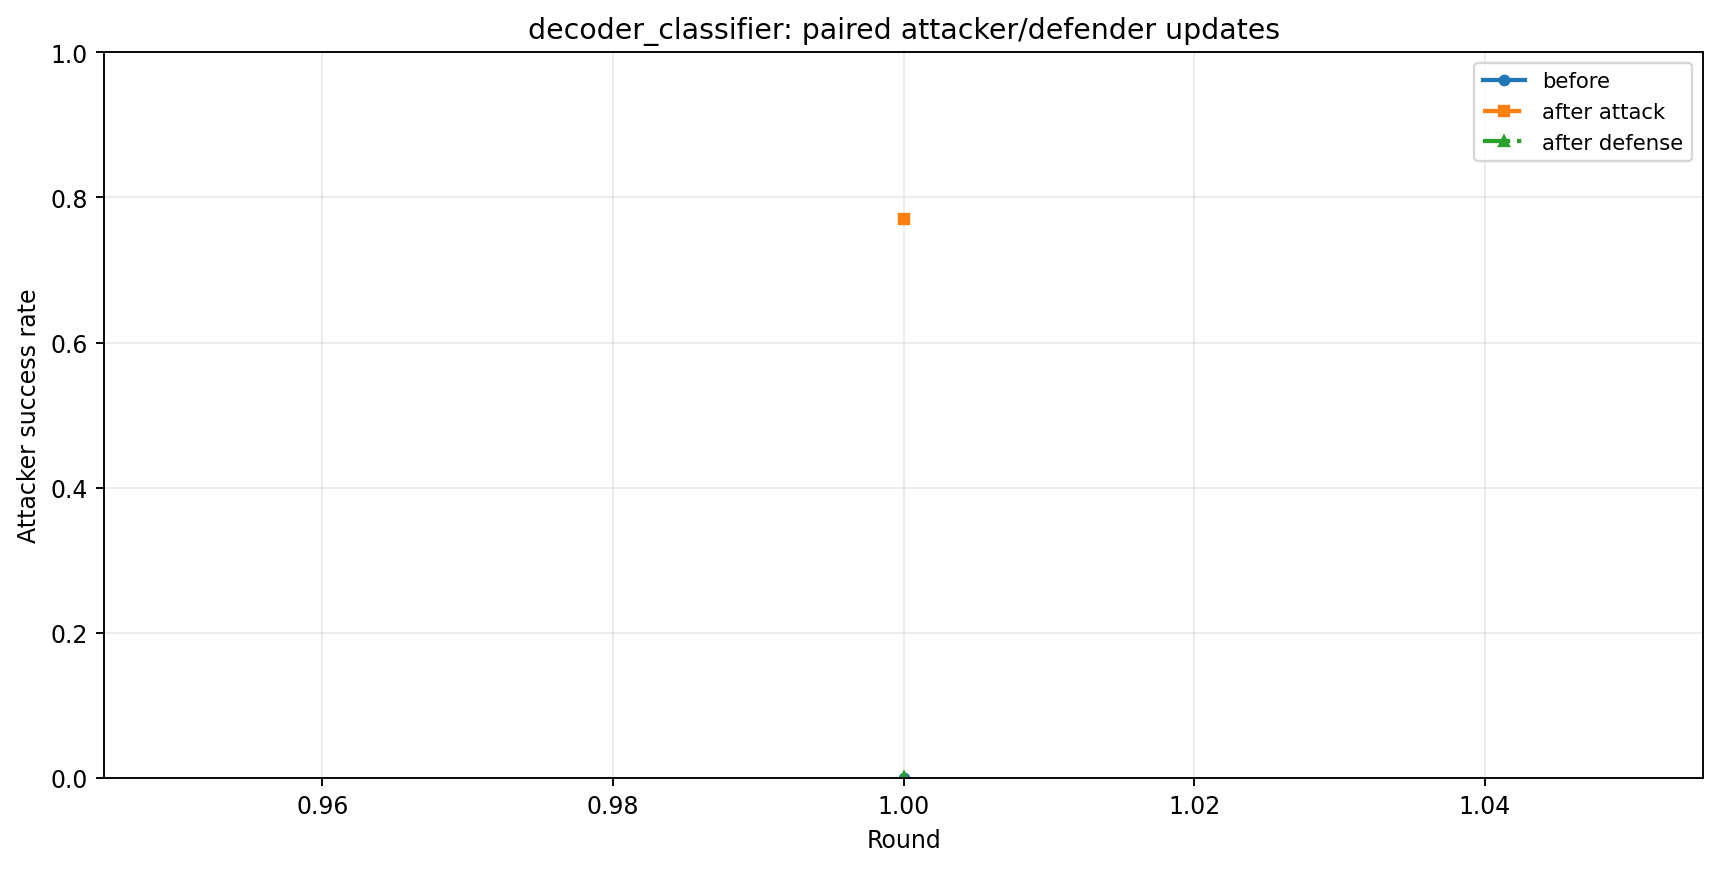
\includegraphics[keepaspectratio,alt={The after-attack and after-defense measurements reuse identical generated texts.}]{../docs/figures/research/race100-20261022T135029612516Z-ensemble-decoder_classifier.png}}
\caption{The after-attack and after-defense measurements reuse identical
generated texts.}
\end{recordfigure}

The after-attack and after-defense measurements reuse identical
generated texts.
\href{../docs/figures/research/race100-20261022T135029612516Z-ensemble-decoder_classifier.csv}{Source
CSV} ·
\href{../docs/figures/research/race100-20261022T135029612516Z-ensemble-decoder_classifier.svg}{Vector
SVG}

\begin{recordfigure}
\centering
\pandocbounded{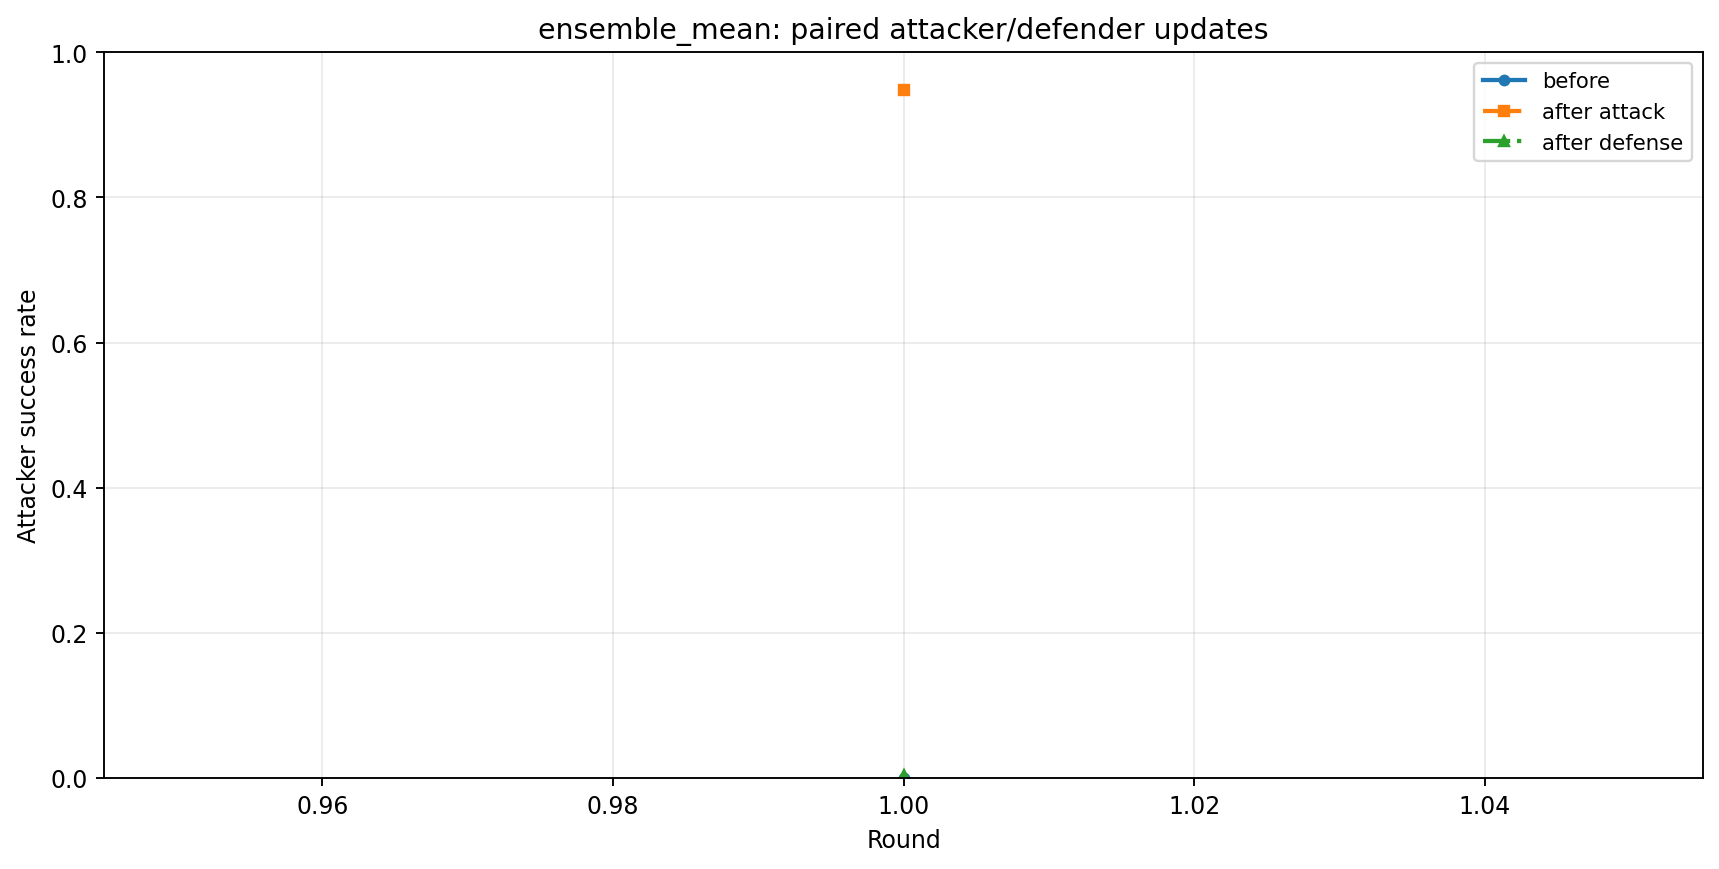
\includegraphics[keepaspectratio,alt={The after-attack and after-defense measurements reuse identical generated texts.}]{../docs/figures/research/race100-20261022T135029612516Z-ensemble-ensemble_mean.png}}
\caption{The after-attack and after-defense measurements reuse identical
generated texts.}
\end{recordfigure}

The after-attack and after-defense measurements reuse identical
generated texts.
\href{../docs/figures/research/race100-20261022T135029612516Z-ensemble-ensemble_mean.csv}{Source
CSV} ·
\href{../docs/figures/research/race100-20261022T135029612516Z-ensemble-ensemble_mean.svg}{Vector
SVG}

Round-one checkpoint reuse: Retained attacker; begin with its first
defender update.

These are single-seed results. Successful warm-up and robustness must be
assessed from the measurements; neither is guaranteed by the training
procedure.

{\scriptsize\setlength{\tabcolsep}{3pt}\def\LTcaptype{none} % do not increment counter
\begin{longtable}[]{@{}
  >{\raggedright\arraybackslash}p{(\linewidth - 10\tabcolsep) * \real{0.1667}}
  >{\raggedright\arraybackslash}p{(\linewidth - 10\tabcolsep) * \real{0.1667}}
  >{\raggedright\arraybackslash}p{(\linewidth - 10\tabcolsep) * \real{0.1667}}
  >{\raggedright\arraybackslash}p{(\linewidth - 10\tabcolsep) * \real{0.1667}}
  >{\raggedright\arraybackslash}p{(\linewidth - 10\tabcolsep) * \real{0.1667}}
  >{\raggedright\arraybackslash}p{(\linewidth - 10\tabcolsep) * \real{0.1667}}@{}}
\toprule\noalign{}
\begin{minipage}[b]{\linewidth}\raggedright
round
\end{minipage} & \begin{minipage}[b]{\linewidth}\raggedright
phase
\end{minipage} & \begin{minipage}[b]{\linewidth}\raggedright
detector
\end{minipage} & \begin{minipage}[b]{\linewidth}\raggedright
attack\_\allowbreak{}success\_\allowbreak{}rate
\end{minipage} & \begin{minipage}[b]{\linewidth}\raggedright
ai\_\allowbreak{}detection\_\allowbreak{}rate
\end{minipage} & \begin{minipage}[b]{\linewidth}\raggedright
human\_\allowbreak{}false\_\allowbreak{}positive\_\allowbreak{}rate
\end{minipage} \\
\midrule\noalign{}
\endhead
\bottomrule\noalign{}
\endlastfoot
1 & before & binoculars & 0.0140 & 0.9860 & 0.0080 \\
1 & before & fast\_\allowbreak{}detect\_\allowbreak{}gpt & 0.0000 &
1.0000 & 0.0000 \\
1 & before & diveye & 0.0280 & 0.9720 & 0.0280 \\
1 & before & roberta & 0.0000 & 1.0000 & 0.0340 \\
1 & before & tfidf & 0.1140 & 0.8860 & 0.0180 \\
1 & before & modernbert\_\allowbreak{}large & 0.0100 & 0.9900 &
0.0160 \\
1 & before & decoder\_\allowbreak{}classifier & 0.0000 & 1.0000 &
0.0000 \\
1 & after\_\allowbreak{}attack & binoculars & 0.9400 & 0.0600 &
0.0080 \\
1 & after\_\allowbreak{}attack &
fast\_\allowbreak{}detect\_\allowbreak{}gpt & 0.9300 & 0.0700 &
0.0000 \\
1 & after\_\allowbreak{}attack & diveye & 0.8100 & 0.1900 & 0.0280 \\
1 & after\_\allowbreak{}attack & roberta & 0.9220 & 0.0780 & 0.0340 \\
1 & after\_\allowbreak{}attack & tfidf & 0.9660 & 0.0340 & 0.0180 \\
1 & after\_\allowbreak{}attack & modernbert\_\allowbreak{}large & 0.9800
& 0.0200 & 0.0160 \\
1 & after\_\allowbreak{}attack & decoder\_\allowbreak{}classifier &
0.7700 & 0.2300 & 0.0000 \\
1 & after\_\allowbreak{}defense & binoculars & 0.0060 & 0.9940 &
0.0160 \\
1 & after\_\allowbreak{}defense &
fast\_\allowbreak{}detect\_\allowbreak{}gpt & 0.0000 & 1.0000 &
0.0000 \\
1 & after\_\allowbreak{}defense & diveye & 0.0700 & 0.9300 & 0.0580 \\
1 & after\_\allowbreak{}defense & roberta & 0.0080 & 0.9920 & 0.0020 \\
1 & after\_\allowbreak{}defense & tfidf & 0.0580 & 0.9420 & 0.0700 \\
1 & after\_\allowbreak{}defense & modernbert\_\allowbreak{}large &
0.0080 & 0.9920 & 0.0160 \\
1 & after\_\allowbreak{}defense & decoder\_\allowbreak{}classifier &
0.0020 & 0.9980 & 0.0000 \\
\end{longtable}
}

{\scriptsize\setlength{\tabcolsep}{3pt}\def\LTcaptype{none} % do not increment counter
\begin{longtable}[]{@{}
  >{\raggedright\arraybackslash}p{(\linewidth - 10\tabcolsep) * \real{0.1667}}
  >{\raggedright\arraybackslash}p{(\linewidth - 10\tabcolsep) * \real{0.1667}}
  >{\raggedright\arraybackslash}p{(\linewidth - 10\tabcolsep) * \real{0.1667}}
  >{\raggedright\arraybackslash}p{(\linewidth - 10\tabcolsep) * \real{0.1667}}
  >{\raggedright\arraybackslash}p{(\linewidth - 10\tabcolsep) * \real{0.1667}}
  >{\raggedright\arraybackslash}p{(\linewidth - 10\tabcolsep) * \real{0.1667}}@{}}
\toprule\noalign{}
\begin{minipage}[b]{\linewidth}\raggedright
round
\end{minipage} & \begin{minipage}[b]{\linewidth}\raggedright
phase
\end{minipage} & \begin{minipage}[b]{\linewidth}\raggedright
detector
\end{minipage} & \begin{minipage}[b]{\linewidth}\raggedright
roc\_\allowbreak{}auc
\end{minipage} & \begin{minipage}[b]{\linewidth}\raggedright
semantic\_\allowbreak{}similarity
\end{minipage} & \begin{minipage}[b]{\linewidth}\raggedright
num\_\allowbreak{}generated
\end{minipage} \\
\midrule\noalign{}
\endhead
\bottomrule\noalign{}
\endlastfoot
1 & before & binoculars & 0.9998 & undefined & 500 \\
1 & before & fast\_\allowbreak{}detect\_\allowbreak{}gpt & 1.0000 &
undefined & 500 \\
1 & before & diveye & 0.9970 & undefined & 500 \\
1 & before & roberta & 0.9983 & undefined & 500 \\
1 & before & tfidf & 0.9834 & undefined & 500 \\
1 & before & modernbert\_\allowbreak{}large & 0.9992 & undefined &
500 \\
1 & before & decoder\_\allowbreak{}classifier & 1.0000 & undefined &
500 \\
1 & after\_\allowbreak{}attack & binoculars & 0.6103 & 0.8701 & 500 \\
1 & after\_\allowbreak{}attack &
fast\_\allowbreak{}detect\_\allowbreak{}gpt & 0.4984 & 0.8701 & 500 \\
1 & after\_\allowbreak{}attack & diveye & 0.7795 & 0.8701 & 500 \\
1 & after\_\allowbreak{}attack & roberta & 0.5555 & 0.8701 & 500 \\
1 & after\_\allowbreak{}attack & tfidf & 0.3939 & 0.8701 & 500 \\
1 & after\_\allowbreak{}attack & modernbert\_\allowbreak{}large & 0.6956
& 0.8701 & 500 \\
1 & after\_\allowbreak{}attack & decoder\_\allowbreak{}classifier &
0.9150 & 0.8701 & 500 \\
1 & after\_\allowbreak{}defense & binoculars & 0.9997 & 0.8701 & 500 \\
1 & after\_\allowbreak{}defense &
fast\_\allowbreak{}detect\_\allowbreak{}gpt & 1.0000 & 0.8701 & 500 \\
1 & after\_\allowbreak{}defense & diveye & 0.9829 & 0.8701 & 500 \\
1 & after\_\allowbreak{}defense & roberta & 0.9999 & 0.8701 & 500 \\
1 & after\_\allowbreak{}defense & tfidf & 0.9432 & 0.8701 & 500 \\
1 & after\_\allowbreak{}defense & modernbert\_\allowbreak{}large &
0.9991 & 0.8701 & 500 \\
1 & after\_\allowbreak{}defense & decoder\_\allowbreak{}classifier &
1.0000 & 0.8701 & 500 \\
\end{longtable}
}

{\scriptsize\setlength{\tabcolsep}{3pt}\def\LTcaptype{none} % do not increment counter
\begin{longtable}[]{@{}
  >{\raggedright\arraybackslash}p{(\linewidth - 6\tabcolsep) * \real{0.2500}}
  >{\raggedright\arraybackslash}p{(\linewidth - 6\tabcolsep) * \real{0.2500}}
  >{\raggedright\arraybackslash}p{(\linewidth - 6\tabcolsep) * \real{0.2500}}
  >{\raggedright\arraybackslash}p{(\linewidth - 6\tabcolsep) * \real{0.2500}}@{}}
\toprule\noalign{}
\begin{minipage}[b]{\linewidth}\raggedright
round
\end{minipage} & \begin{minipage}[b]{\linewidth}\raggedright
phase
\end{minipage} & \begin{minipage}[b]{\linewidth}\raggedright
detector
\end{minipage} & \begin{minipage}[b]{\linewidth}\raggedright
num\_\allowbreak{}ineligible\_\allowbreak{}pairs
\end{minipage} \\
\midrule\noalign{}
\endhead
\bottomrule\noalign{}
\endlastfoot
1 & before & binoculars & 0 \\
1 & before & fast\_\allowbreak{}detect\_\allowbreak{}gpt & 0 \\
1 & before & diveye & 0 \\
1 & before & roberta & 0 \\
1 & before & tfidf & 0 \\
1 & before & modernbert\_\allowbreak{}large & 0 \\
1 & before & decoder\_\allowbreak{}classifier & 0 \\
1 & after\_\allowbreak{}attack & binoculars & 0 \\
1 & after\_\allowbreak{}attack &
fast\_\allowbreak{}detect\_\allowbreak{}gpt & 0 \\
1 & after\_\allowbreak{}attack & diveye & 0 \\
1 & after\_\allowbreak{}attack & roberta & 0 \\
1 & after\_\allowbreak{}attack & tfidf & 0 \\
1 & after\_\allowbreak{}attack & modernbert\_\allowbreak{}large & 0 \\
1 & after\_\allowbreak{}attack & decoder\_\allowbreak{}classifier & 0 \\
1 & after\_\allowbreak{}defense & binoculars & 0 \\
1 & after\_\allowbreak{}defense &
fast\_\allowbreak{}detect\_\allowbreak{}gpt & 0 \\
1 & after\_\allowbreak{}defense & diveye & 0 \\
1 & after\_\allowbreak{}defense & roberta & 0 \\
1 & after\_\allowbreak{}defense & tfidf & 0 \\
1 & after\_\allowbreak{}defense & modernbert\_\allowbreak{}large & 0 \\
1 & after\_\allowbreak{}defense & decoder\_\allowbreak{}classifier &
0 \\
\end{longtable}
}

\subsection{Updated defenders on the base
model}\label{record-docs-research-results-md-updated-defenders-on-the-base-model}

This check reuses the original 500 reserved base-Qwen outputs and 500
human passages. It generates no new text and performs no training. The
comparison uses threshold 0.5 before and after the defender update; the
earlier model is the Qwen-warmed defender, before adaptation to the RL
attacker.

gemma: base-Qwen detection changes from 100.0\% to 100.0\%; human false
positives change from 0.0\% to 0.2\%. modernbert: base-Qwen detection
changes from 99.0\% to 90.2\%; human false positives change from 1.6\%
to 0.4\%. ensemble: base-Qwen detection changes from 100.0\% to 98.4\%;
human false positives change from 0.2\% to 0.0\%.

{\scriptsize\setlength{\tabcolsep}{3pt}\def\LTcaptype{none} % do not increment counter
\begin{longtable}[]{@{}
  >{\raggedright\arraybackslash}p{(\linewidth - 10\tabcolsep) * \real{0.1667}}
  >{\raggedright\arraybackslash}p{(\linewidth - 10\tabcolsep) * \real{0.1667}}
  >{\raggedright\arraybackslash}p{(\linewidth - 10\tabcolsep) * \real{0.1667}}
  >{\raggedright\arraybackslash}p{(\linewidth - 10\tabcolsep) * \real{0.1667}}
  >{\raggedright\arraybackslash}p{(\linewidth - 10\tabcolsep) * \real{0.1667}}
  >{\raggedright\arraybackslash}p{(\linewidth - 10\tabcolsep) * \real{0.1667}}@{}}
\toprule\noalign{}
\begin{minipage}[b]{\linewidth}\raggedright
branch
\end{minipage} & \begin{minipage}[b]{\linewidth}\raggedright
detector
\end{minipage} & \begin{minipage}[b]{\linewidth}\raggedright
AI\_\allowbreak{}texts
\end{minipage} & \begin{minipage}[b]{\linewidth}\raggedright
AI\_\allowbreak{}detection\_\allowbreak{}before
\end{minipage} & \begin{minipage}[b]{\linewidth}\raggedright
AI\_\allowbreak{}detection\_\allowbreak{}after
\end{minipage} & \begin{minipage}[b]{\linewidth}\raggedright
human\_\allowbreak{}FPR\_\allowbreak{}before
\end{minipage} \\
\midrule\noalign{}
\endhead
\bottomrule\noalign{}
\endlastfoot
gemma & decoder\_\allowbreak{}classifier & 500 & 1.0000 & 1.0000 &
0.0000 \\
modernbert & modernbert\_\allowbreak{}large & 500 & 0.9900 & 0.9020 &
0.0160 \\
ensemble & binoculars & 500 & 0.9860 & 0.9720 & 0.0080 \\
ensemble & fast\_\allowbreak{}detect\_\allowbreak{}gpt & 500 & 1.0000 &
0.9900 & 0.0000 \\
ensemble & diveye & 500 & 0.9720 & 0.9380 & 0.0280 \\
ensemble & roberta & 500 & 1.0000 & 0.9800 & 0.0340 \\
ensemble & tfidf & 500 & 0.8860 & 0.2820 & 0.0180 \\
ensemble & modernbert\_\allowbreak{}large & 500 & 0.9900 & 0.9640 &
0.0160 \\
ensemble & decoder\_\allowbreak{}classifier & 500 & 1.0000 & 1.0000 &
0.0000 \\
ensemble & ensemble\_\allowbreak{}mean & 500 & 1.0000 & 0.9840 &
0.0020 \\
\end{longtable}
}

{\scriptsize\setlength{\tabcolsep}{3pt}\def\LTcaptype{none} % do not increment counter
\begin{longtable}[]{@{}
  >{\raggedright\arraybackslash}p{(\linewidth - 4\tabcolsep) * \real{0.3333}}
  >{\raggedright\arraybackslash}p{(\linewidth - 4\tabcolsep) * \real{0.3333}}
  >{\raggedright\arraybackslash}p{(\linewidth - 4\tabcolsep) * \real{0.3333}}@{}}
\toprule\noalign{}
\begin{minipage}[b]{\linewidth}\raggedright
branch
\end{minipage} & \begin{minipage}[b]{\linewidth}\raggedright
human\_\allowbreak{}FPR\_\allowbreak{}after
\end{minipage} & \begin{minipage}[b]{\linewidth}\raggedright
AUROC\_\allowbreak{}after
\end{minipage} \\
\midrule\noalign{}
\endhead
\bottomrule\noalign{}
\endlastfoot
gemma & 0.0020 & 1.0000 \\
modernbert & 0.0040 & 0.9972 \\
ensemble & 0.0160 & 0.9990 \\
ensemble & 0.0000 & 0.9999 \\
ensemble & 0.0580 & 0.9855 \\
ensemble & 0.0020 & 0.9972 \\
ensemble & 0.0700 & 0.6158 \\
ensemble & 0.0160 & 0.9981 \\
ensemble & 0.0000 & 1.0000 \\
ensemble & 0.0000 & 1.0000 \\
\end{longtable}
}

The largest observed base-detection decrease is ensemble/tfidf: 88.6\%
to 28.2\%, with post-update human false positives of 7.0\% and AUROC
0.6158. Aggregate ensemble performance can conceal such member-level
losses.

\begin{recordfigure}
\centering
\pandocbounded{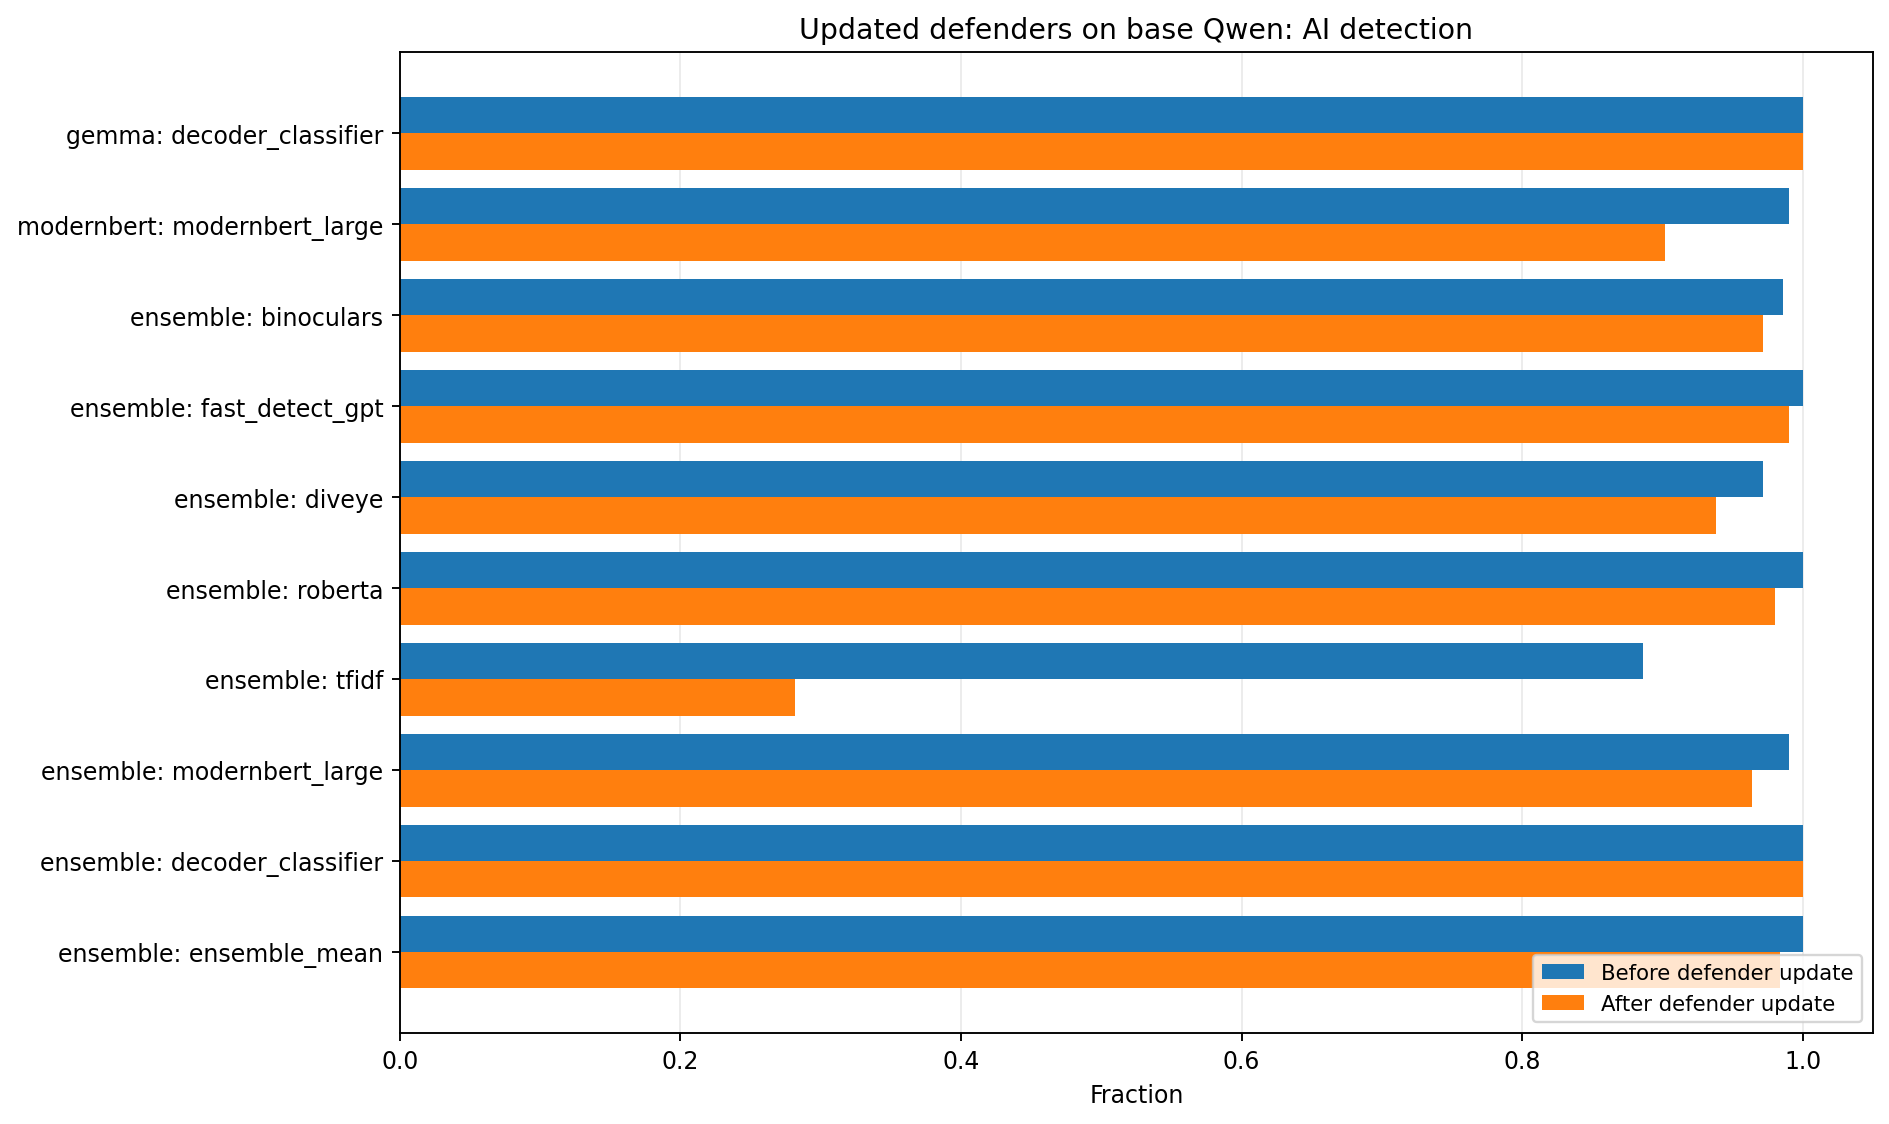
\includegraphics[keepaspectratio,alt={}]{../docs/figures/research/base-retest-20261022T135029612516Z-AI_detection.png}}
\caption{base-retest-20261022T135029612516Z-AI\_\allowbreak{}detection}
\end{recordfigure}

\href{../docs/figures/research/base-retest-20261022T135029612516Z-AI_detection.csv}{Source
CSV} ·
\href{../docs/figures/research/base-retest-20261022T135029612516Z-AI_detection.svg}{Vector
SVG}.

\begin{recordfigure}
\centering
\pandocbounded{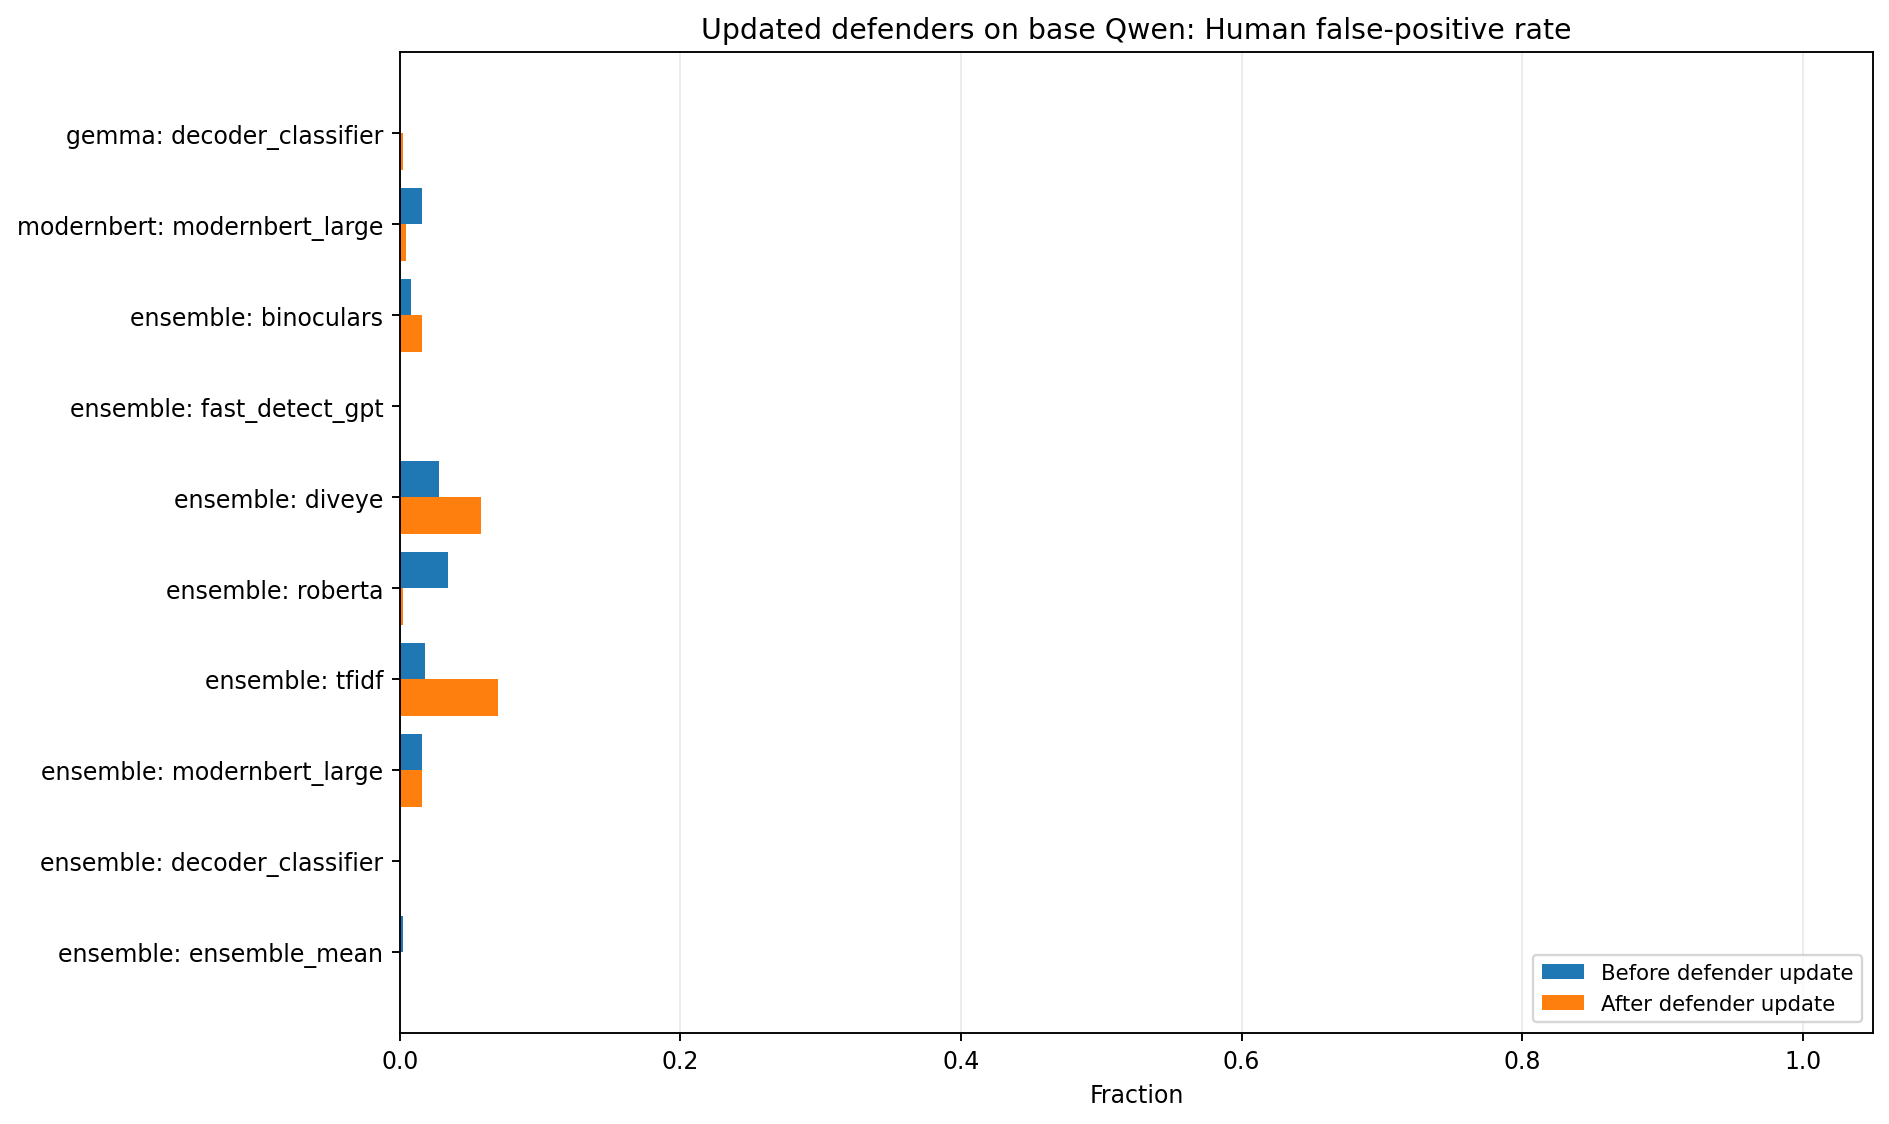
\includegraphics[keepaspectratio,alt={}]{../docs/figures/research/base-retest-20261022T135029612516Z-human_FPR.png}}
\caption{base-retest-20261022T135029612516Z-human\_\allowbreak{}FPR}
\end{recordfigure}

\href{../docs/figures/research/base-retest-20261022T135029612516Z-human_FPR.csv}{Source
CSV} ·
\href{../docs/figures/research/base-retest-20261022T135029612516Z-human_FPR.svg}{Vector
SVG}.

This measures retention on base outputs after learning the fixed RL
attack. A drop in base detection shows that recovering detection on the
RL outputs does not automatically preserve the original operating point.
The human false-positive rate and AUROC help distinguish that tradeoff
from a broad loss of ranking quality. This does not measure robustness
to a new adaptive attacker.

\href{../results/research_workflow/defender_comparison/races_100/20261022T135029612516Z/base_retest/metrics.csv}{Shared
base-evaluation metrics}.

\begin{recordfigure}
\centering
\pandocbounded{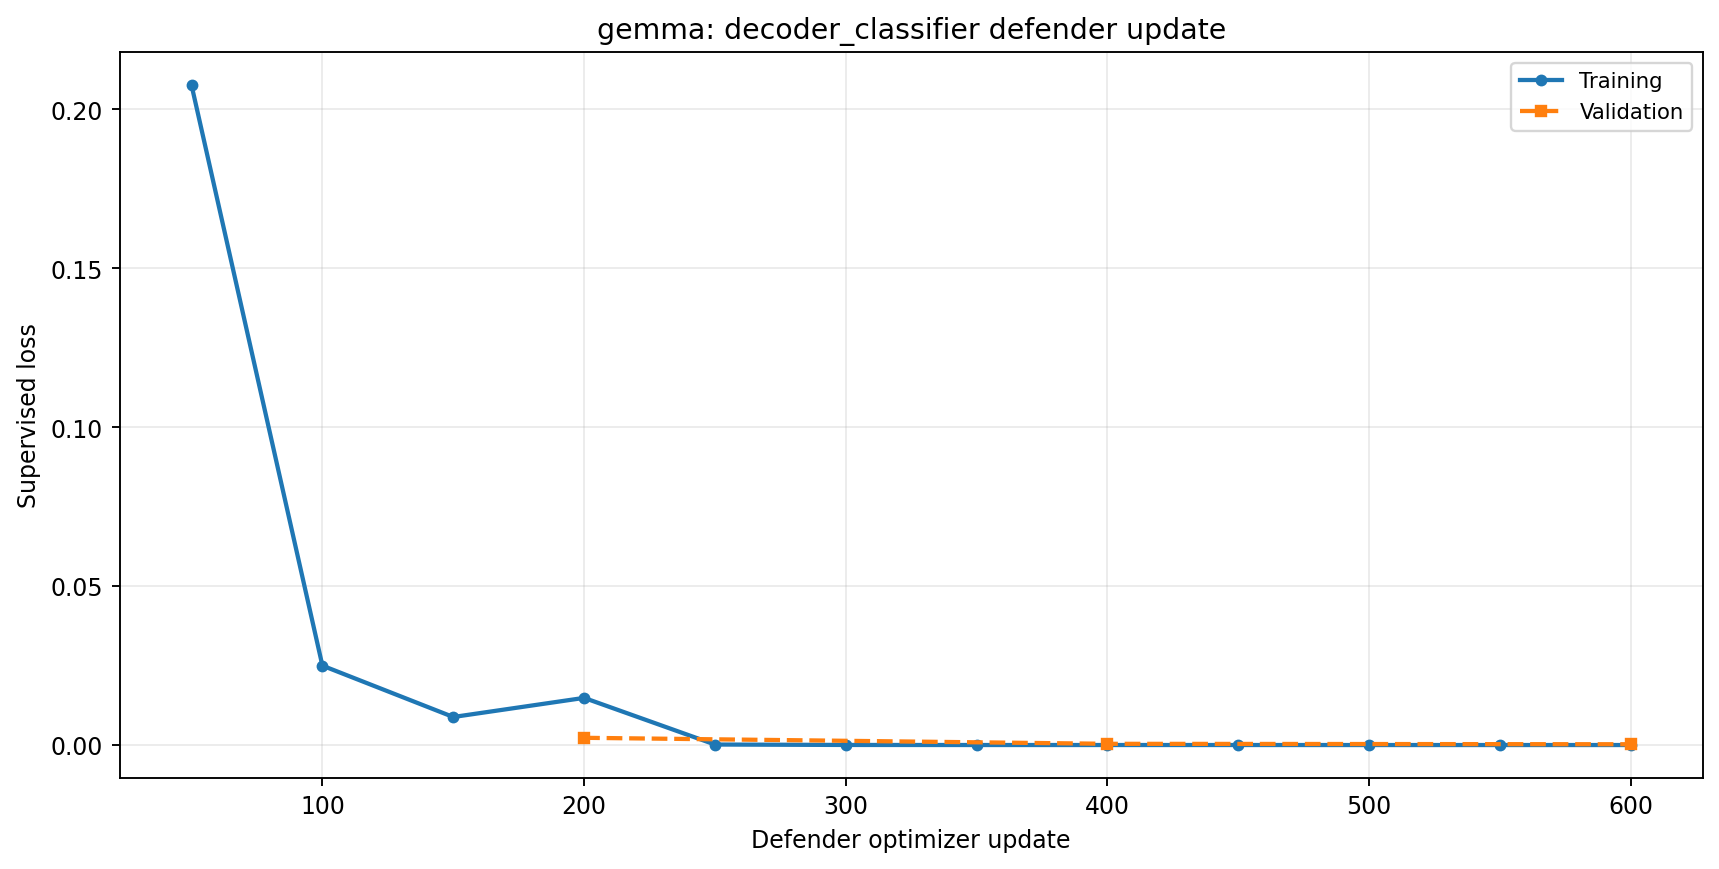
\includegraphics[keepaspectratio,alt={}]{../docs/figures/research/defense-20261022T135029612516Z-gemma-decoder_classifier-loss.png}}
\caption{defense-20261022T135029612516Z-gemma-decoder\_\allowbreak{}classifier-loss}
\end{recordfigure}

\href{../docs/figures/research/defense-20261022T135029612516Z-gemma-decoder_classifier-loss.csv}{Source
CSV} ·
\href{../docs/figures/research/defense-20261022T135029612516Z-gemma-decoder_classifier-loss.svg}{Vector
SVG}.

\begin{recordfigure}
\centering
\pandocbounded{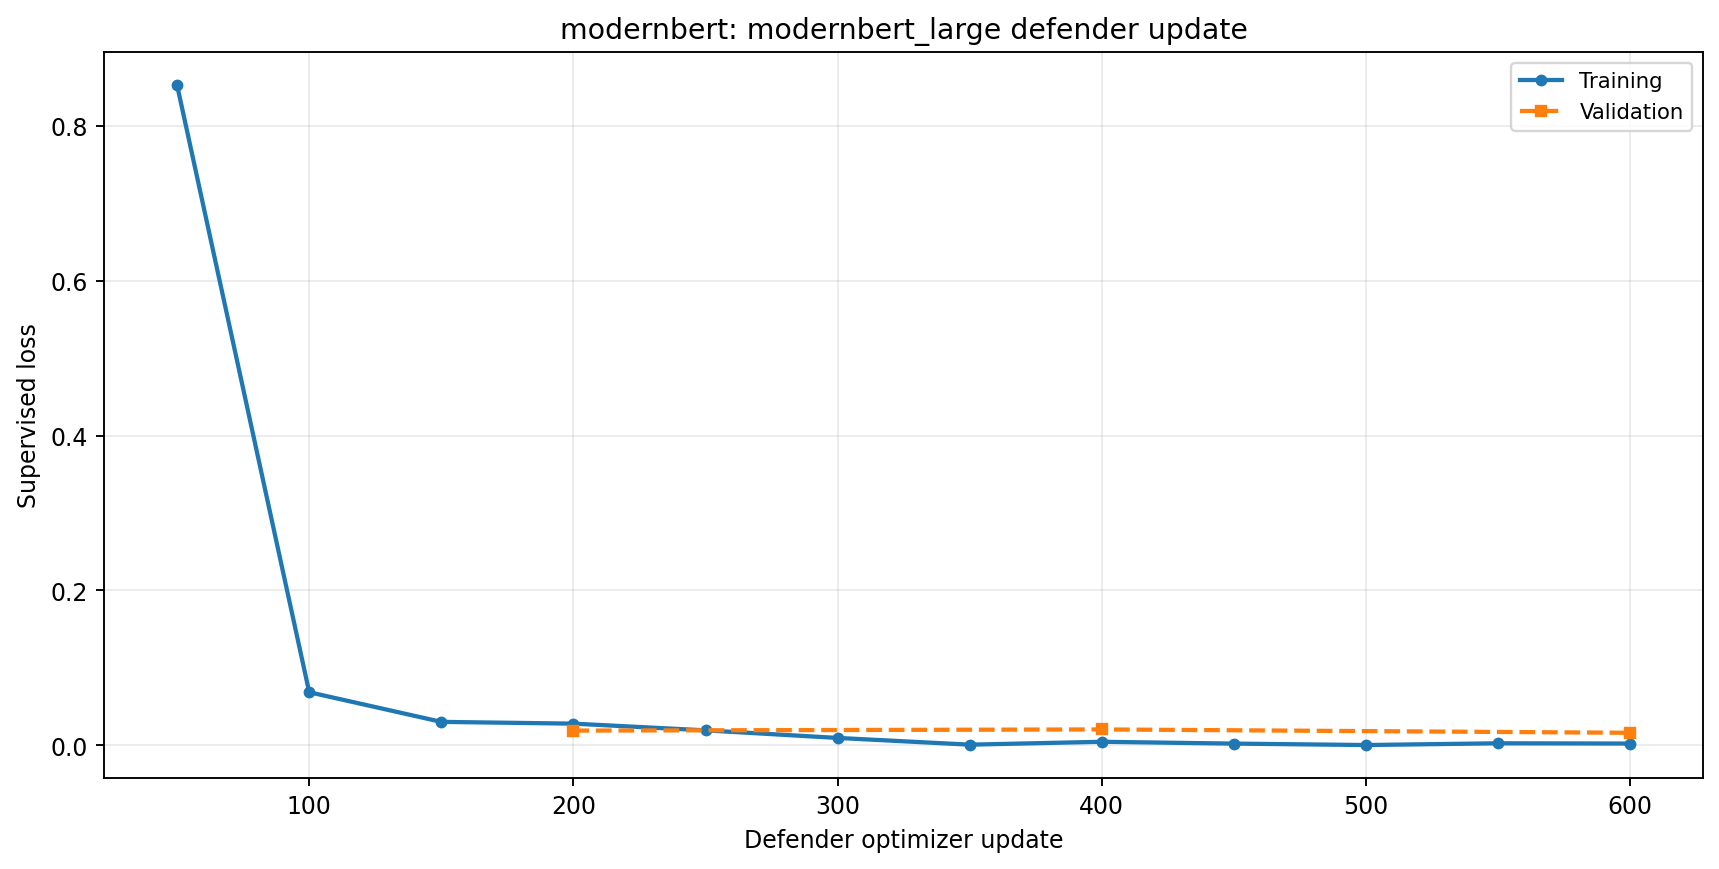
\includegraphics[keepaspectratio,alt={}]{../docs/figures/research/defense-20261022T135029612516Z-modernbert-modernbert_large-loss.png}}
\caption{defense-20261022T135029612516Z-modernbert-modernbert\_\allowbreak{}large-loss}
\end{recordfigure}

\href{../docs/figures/research/defense-20261022T135029612516Z-modernbert-modernbert_large-loss.csv}{Source
CSV} ·
\href{../docs/figures/research/defense-20261022T135029612516Z-modernbert-modernbert_large-loss.svg}{Vector
SVG}.

\begin{recordfigure}
\centering
\pandocbounded{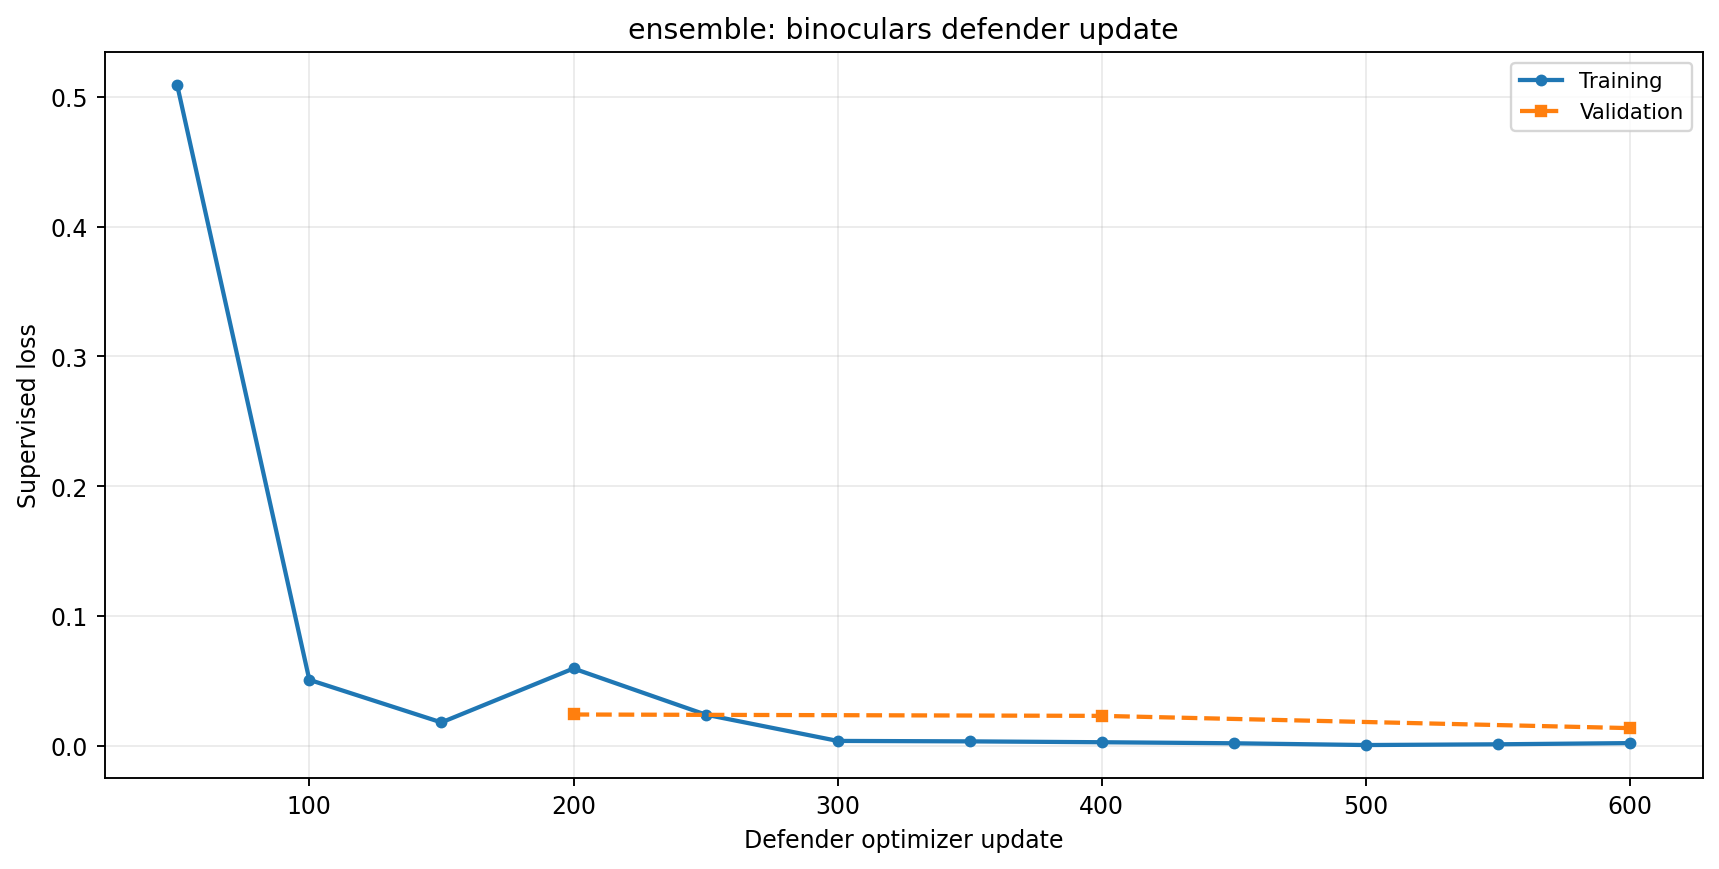
\includegraphics[keepaspectratio,alt={defense-20261022T135029612516Z-ensemble-binoculars-loss}]{../docs/figures/research/defense-20261022T135029612516Z-ensemble-binoculars-loss.png}}
\caption{defense-20261022T135029612516Z-ensemble-binoculars-loss}
\end{recordfigure}

\href{../docs/figures/research/defense-20261022T135029612516Z-ensemble-binoculars-loss.csv}{Source
CSV} ·
\href{../docs/figures/research/defense-20261022T135029612516Z-ensemble-binoculars-loss.svg}{Vector
SVG}.

\begin{recordfigure}
\centering
\pandocbounded{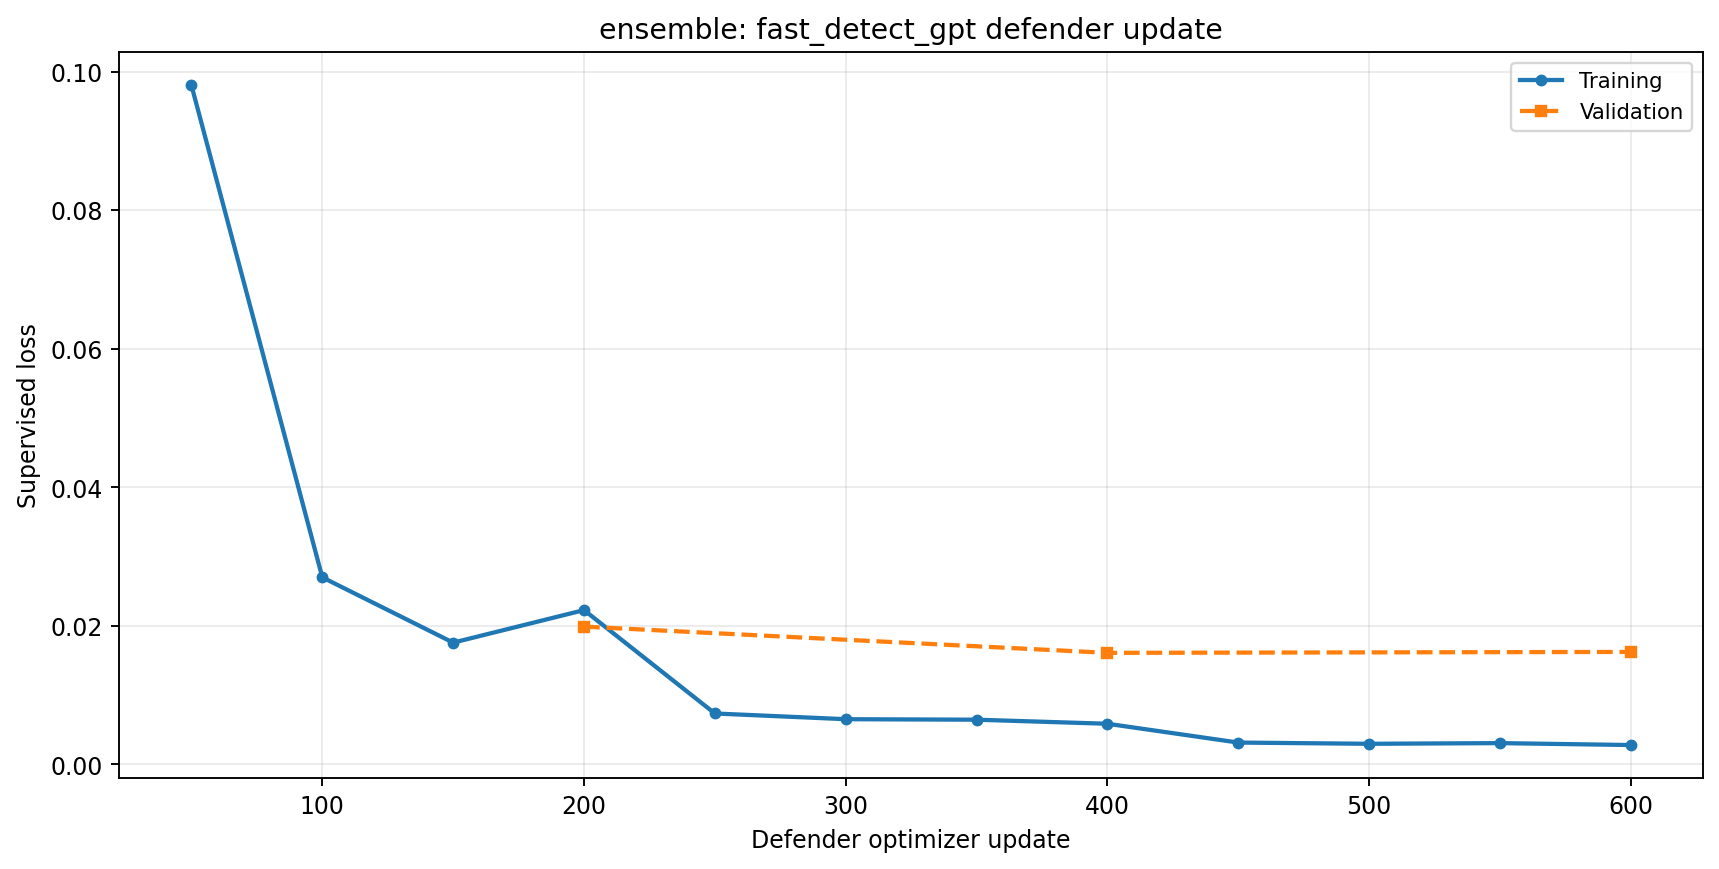
\includegraphics[keepaspectratio,alt={}]{../docs/figures/research/defense-20261022T135029612516Z-ensemble-fast_detect_gpt-loss.png}}
\caption{defense-20261022T135029612516Z-ensemble-fast\_\allowbreak{}detect\_\allowbreak{}gpt-loss}
\end{recordfigure}

\href{../docs/figures/research/defense-20261022T135029612516Z-ensemble-fast_detect_gpt-loss.csv}{Source
CSV} ·
\href{../docs/figures/research/defense-20261022T135029612516Z-ensemble-fast_detect_gpt-loss.svg}{Vector
SVG}.

\begin{recordfigure}
\centering
\pandocbounded{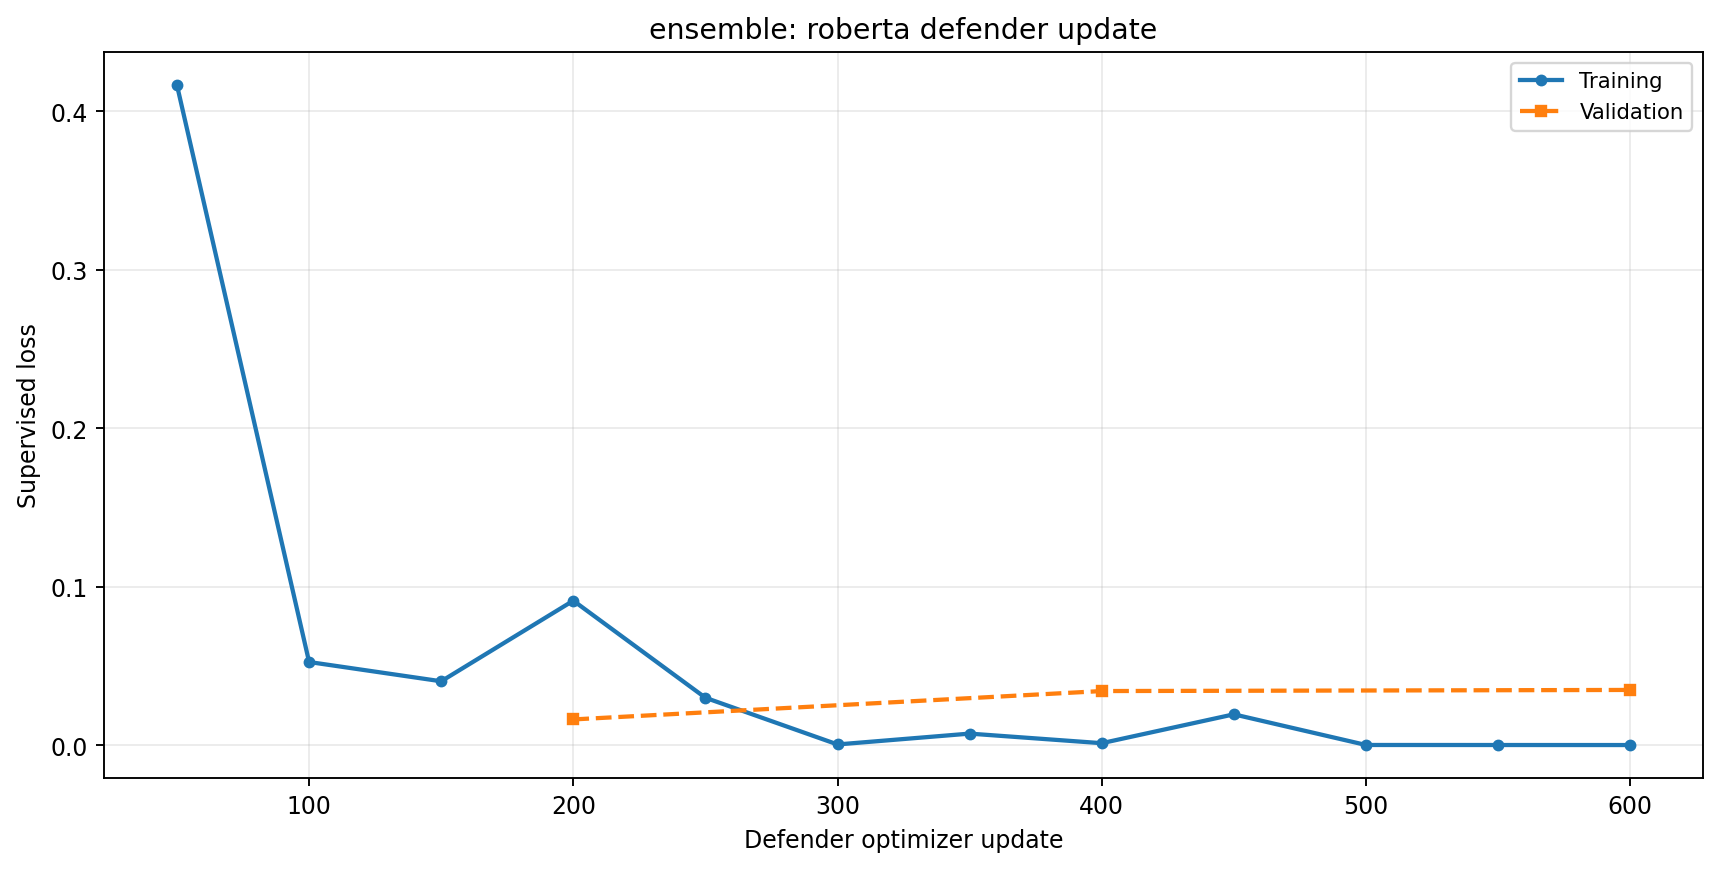
\includegraphics[keepaspectratio,alt={defense-20261022T135029612516Z-ensemble-roberta-loss}]{../docs/figures/research/defense-20261022T135029612516Z-ensemble-roberta-loss.png}}
\caption{defense-20261022T135029612516Z-ensemble-roberta-loss}
\end{recordfigure}

\href{../docs/figures/research/defense-20261022T135029612516Z-ensemble-roberta-loss.csv}{Source
CSV} ·
\href{../docs/figures/research/defense-20261022T135029612516Z-ensemble-roberta-loss.svg}{Vector
SVG}.

\begin{recordfigure}
\centering
\pandocbounded{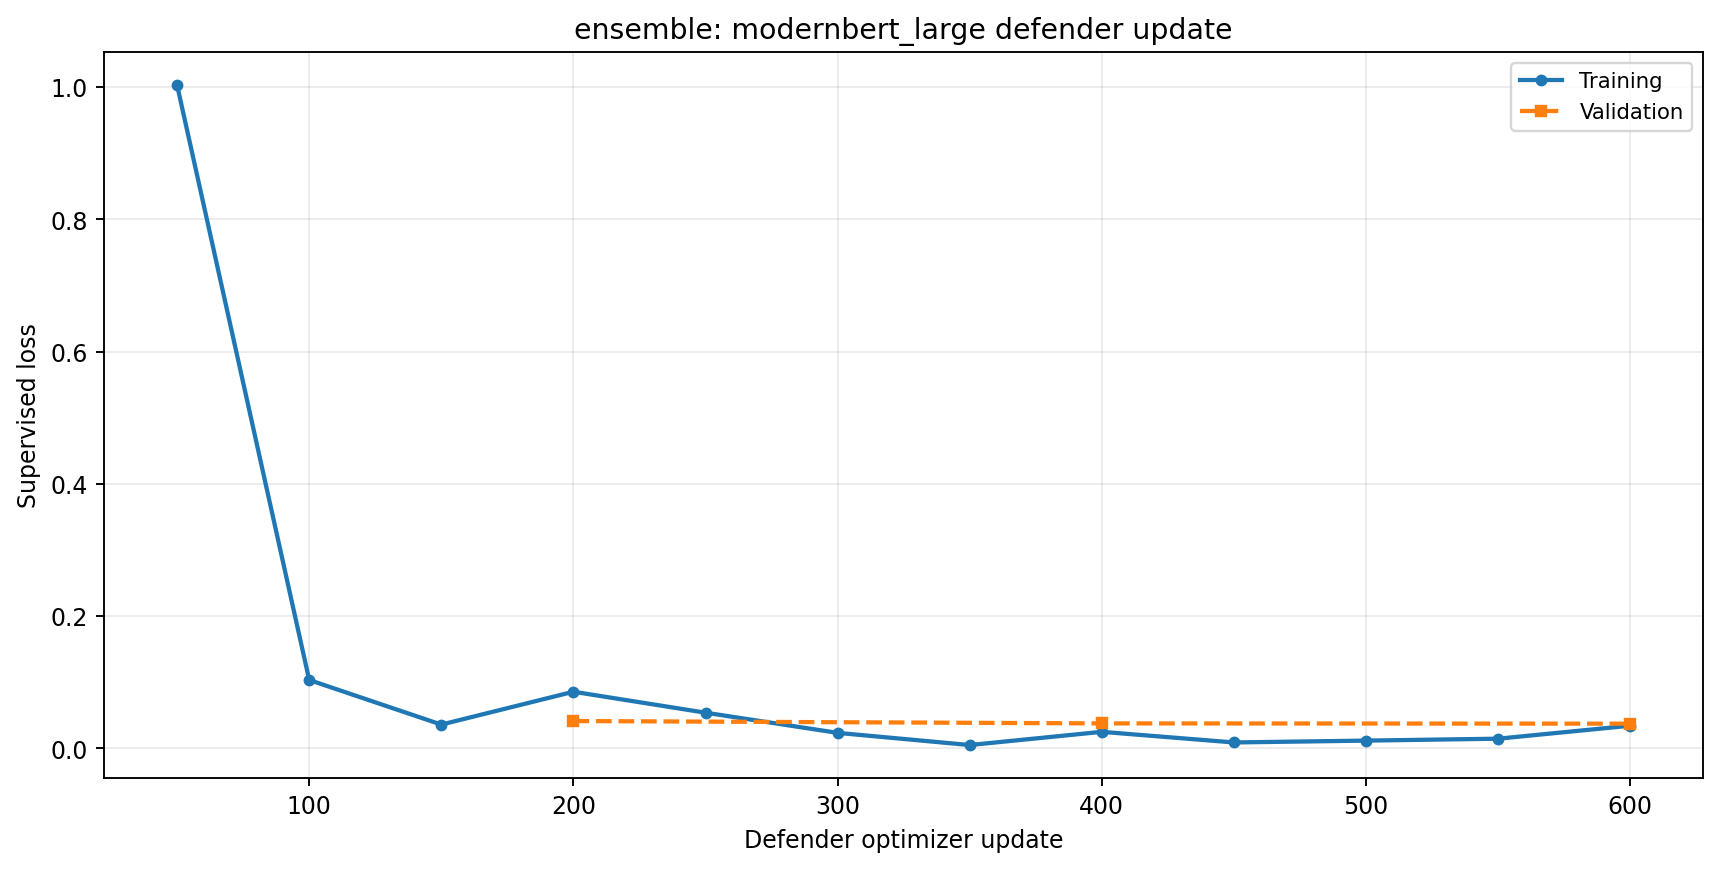
\includegraphics[keepaspectratio,alt={}]{../docs/figures/research/defense-20261022T135029612516Z-ensemble-modernbert_large-loss.png}}
\caption{defense-20261022T135029612516Z-ensemble-modernbert\_\allowbreak{}large-loss}
\end{recordfigure}

\href{../docs/figures/research/defense-20261022T135029612516Z-ensemble-modernbert_large-loss.csv}{Source
CSV} ·
\href{../docs/figures/research/defense-20261022T135029612516Z-ensemble-modernbert_large-loss.svg}{Vector
SVG}.

\begin{recordfigure}
\centering
\pandocbounded{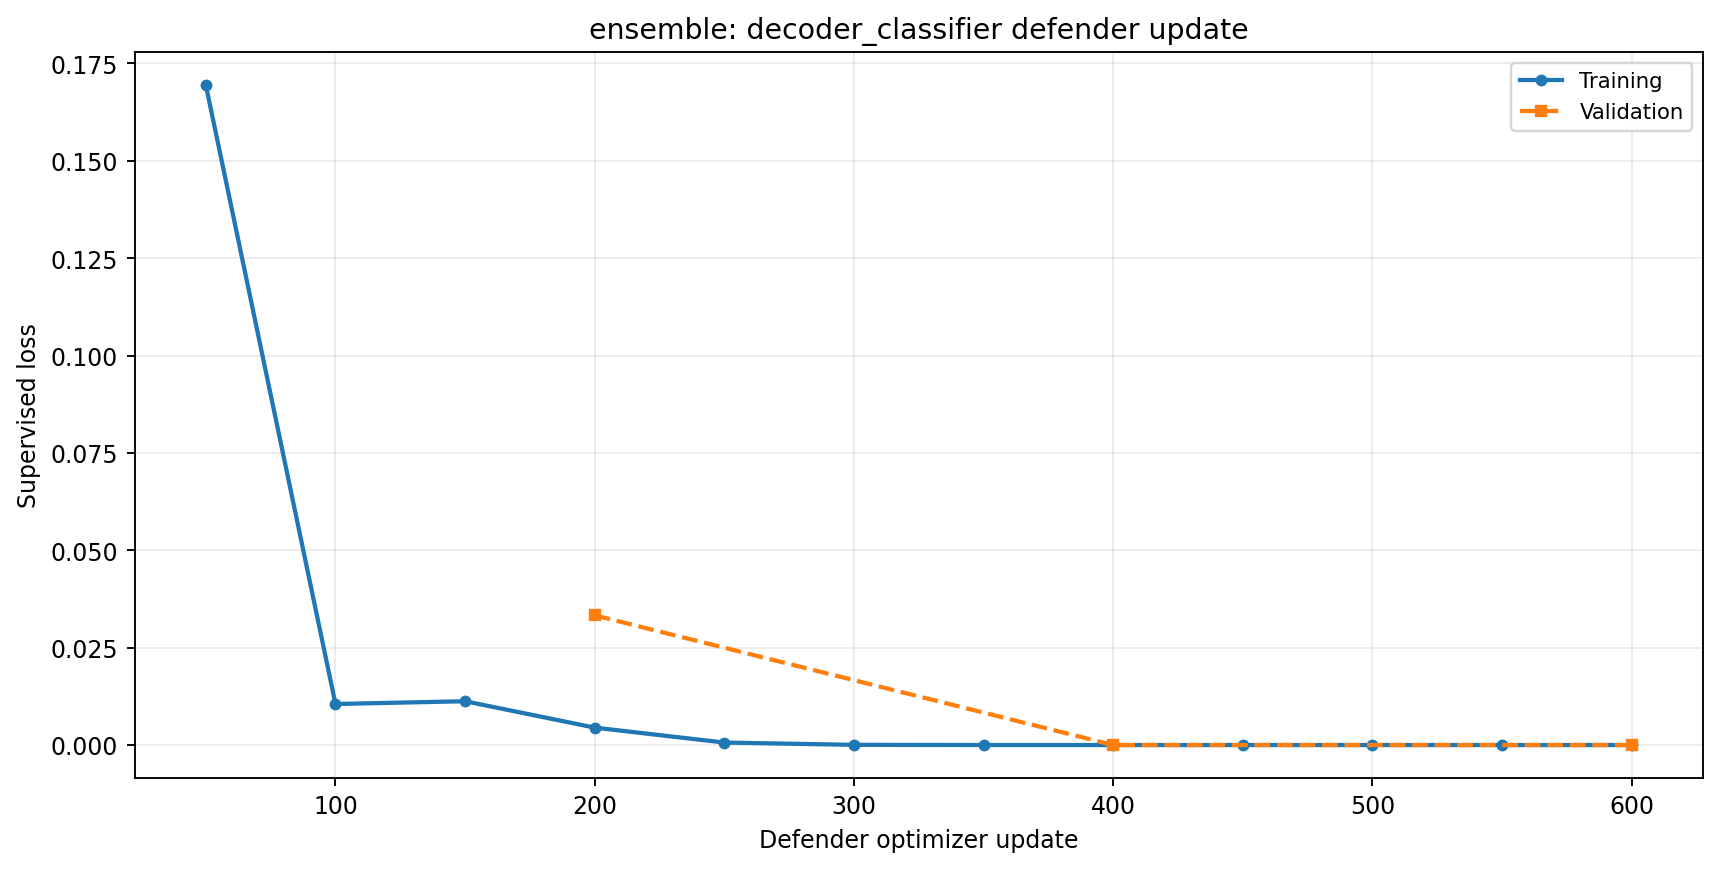
\includegraphics[keepaspectratio,alt={}]{../docs/figures/research/defense-20261022T135029612516Z-ensemble-decoder_classifier-loss.png}}
\caption{defense-20261022T135029612516Z-ensemble-decoder\_\allowbreak{}classifier-loss}
\end{recordfigure}

\href{../docs/figures/research/defense-20261022T135029612516Z-ensemble-decoder_classifier-loss.csv}{Source
CSV} ·
\href{../docs/figures/research/defense-20261022T135029612516Z-ensemble-decoder_classifier-loss.svg}{Vector
SVG}.
